\documentclass[10pt, landscape]{article}
\usepackage[scaled=0.92]{helvet}
\usepackage{calc}
\usepackage{multicol}
\usepackage[a4paper,margin=3mm,landscape]{geometry}
\usepackage{amsmath,amsthm,amsfonts,amssymb}
\usepackage{color,graphicx,overpic}
\usepackage{dsfont}
\usepackage{hyperref}
\usepackage{newtxtext} 
\usepackage{enumitem}
\usepackage{esdiff}
\usepackage[table, dvipsnames]{xcolor}
\usepackage{mathtools}
\setlist{nosep}
\usepackage{tikz}
\usetikzlibrary{shapes.geometric}
\usepackage{makecell}  % for line break withih tabular
\usepackage{ulem}
\usepackage{calrsfs}
\normalem

% for including images
\graphicspath{ {./images/} }

\pdfinfo{
  /Title (nlp-final.pdf)
  /Creator (TeX)
  /Producer (pdfTeX 1.40.0)
  /Author (Yu Chenbo)
  /Subject (CS4248)
/Keywords (CS4248, nlp, nus, cheatsheet, pdf)}

% Turn off header and footer
\pagestyle{empty}

% redefine section commands to use less space
\makeatletter
\renewcommand{\section}{\@startsection{section}{1}{0mm}%
  {-1ex plus -.5ex minus -.2ex}%
  {0.5ex plus .2ex}%x
{\normalfont\large\bfseries}}
\renewcommand{\subsection}{\@startsection{subsection}{2}{0mm}%
  {-1explus -.5ex minus -.2ex}%
  {0.5ex plus .2ex}%
{\normalfont\normalsize\bfseries}}
\renewcommand{\subsubsection}{\@startsection{subsubsection}{3}{0mm}%
  {-1ex plus -.5ex minus -.2ex}%
  {-1ex plus .2ex}%
{\normalfont\small\bfseries\itshape}}%
\makeatother

\renewcommand{\familydefault}{\sfdefault}
\renewcommand\rmdefault{\sfdefault}
%  makes nested numbering (e.g. 1.1.1, 1.1.2, etc)
\renewcommand{\labelenumii}{\theenumii}
\renewcommand{\theenumii}{\theenumi.\arabic{enumii}.}
\renewcommand\labelitemii{•}
\renewcommand\labelitemiii{•}

\definecolor{mathblue}{cmyk}{1,.72,0,.38}
\everymath\expandafter{\the\everymath \color{mathblue} }

% Don't print section numbers
\setcounter{secnumdepth}{0}

\setlength{\parindent}{0pt}
\setlength{\parskip}{0pt plus 0.5ex}
%% this changes all items (enumerate and itemize)
\setlength{\leftmargini}{0.5cm}
\setlength{\leftmarginii}{0.5cm}
\setlist[itemize,1]{leftmargin=2mm,labelindent=1mm,labelsep=1mm}
\setlist[itemize,2]{leftmargin=2mm,labelindent=1mm,labelsep=1mm}
\setlist[itemize,3]{leftmargin=2mm,labelindent=1mm,labelsep=1mm}
\setlist[enumerate,1]{leftmargin=4mm,labelindent=1mm,labelsep=1mm}
\setlist[enumerate,2]{leftmargin=4mm,labelindent=1mm,labelsep=1mm}
\setlist[enumerate,3]{leftmargin=4mm,labelindent=1mm,labelsep=1mm}

% adding my commands
\input{../Latex/Util/style-helpers.tex}
\input{../Latex/Util/code.tex}
\input{../Latex/Util/math.tex}
\input{../Latex/Util/joins.tex}

% aliasing commands
\newcommand{\eps}{\varepsilon}
% \newcommand{\ta}{\textbf{a}}
% \newcommand{\tb}{\textbf{b}}
% \newcommand{\tc}{\textbf{c}}
% \newcommand{\tr}{\textbf{r}}

\DeclareMathOperator*{\argmax}{arg\,max}
\DeclareMathOperator*{\argmin}{arg\,min}

% -----------------------------------------------------------------------

\begin{document}
\raggedright
\begin{multicols*}{3}
  \begin{center}
    \fbox{%
    \parbox{0.8\linewidth}{\centering \textcolor{black}{
      {\Large\textbf{CS4248}}
      \\ \normalsize{AY24/25 SEM 2}}
    \\ {\footnotesize \textcolor{gray}{yyccbb}}
    }%
    }
  \end{center}

  \section{1 - Introduction}
  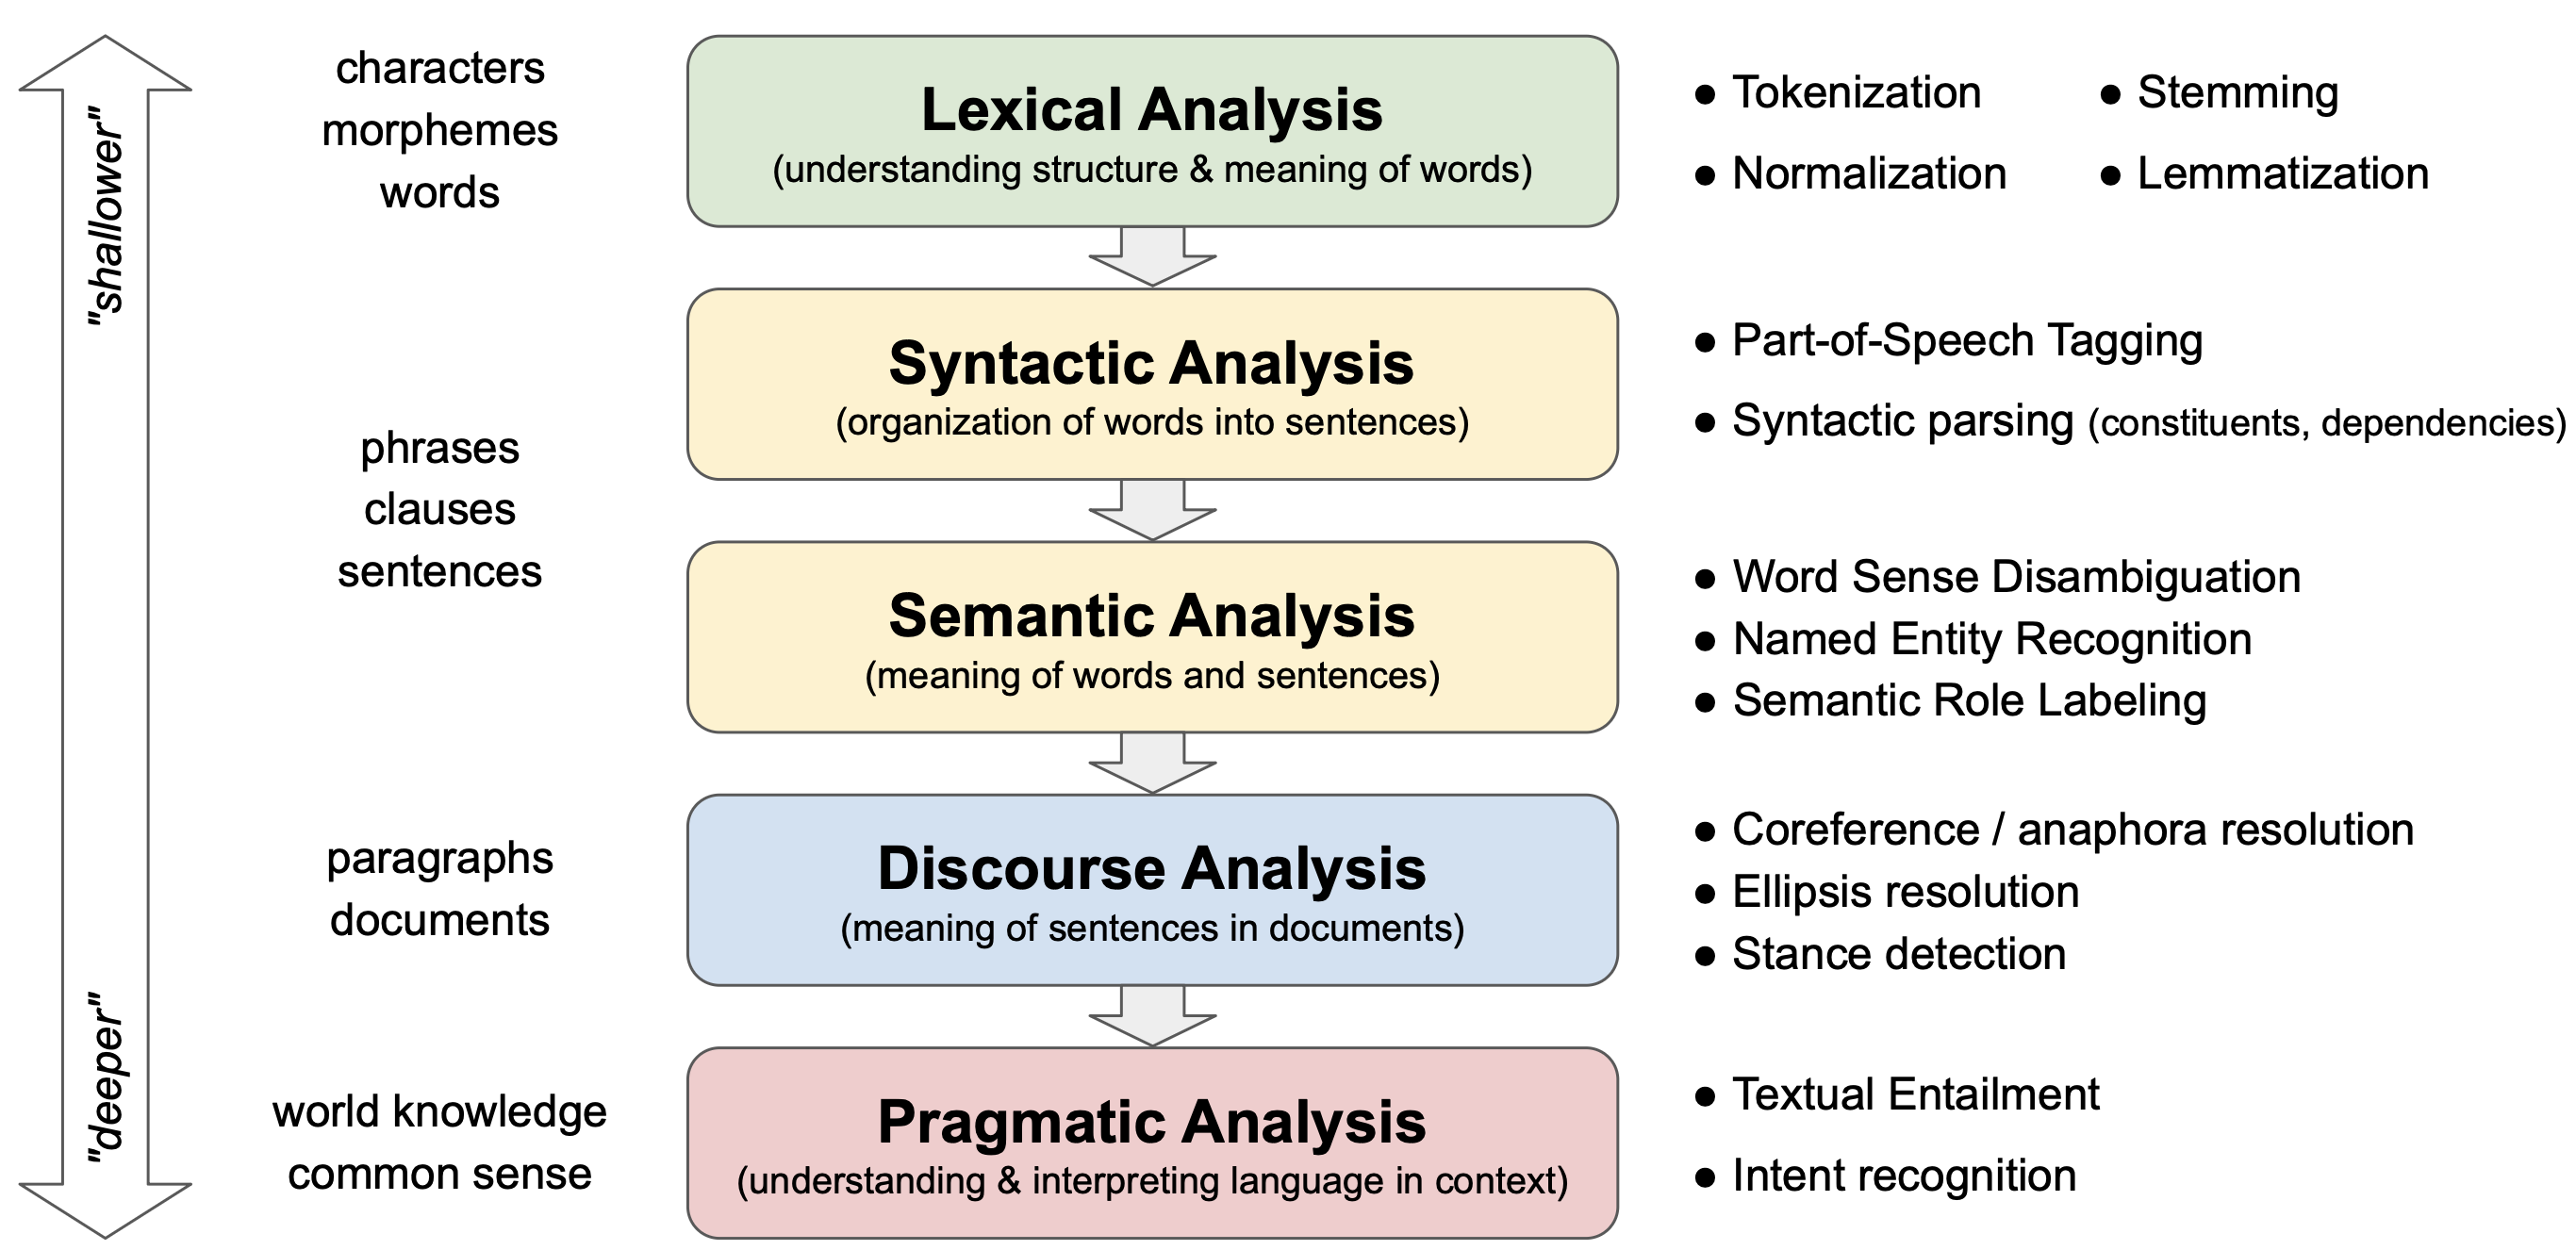
\includegraphics[width=\linewidth]{cs4248-intro-core.png}
  \begin{itemize}
    \item Building blocks of written language: character, morpheme (smallest meaning-bearing unit in a language, e.g. re-act-ion), word, phrase, clause (phrase with a subject and a verb), sentence, paragraph, document, corpus (collection of documents).
    \item Morphology: study of the forms \& formation of words in a language.
    \item \begin{itemize}
      \item Free morphemes: (stems) can stand alone as its own word.
      \item Bound morphemes: derivational (change the semantic meaning or POS of the word, e.g. un-, -er as in noun, -less), inflectional (assign a grammatical property, e.g. -ed, -s,-'s, -er as in comparative form)
    \end{itemize}
    \item Fundamental tasks: lexical analysis---tokenization, syntactic analysis---POS tagging, syntactic parsing, semantic analysis---word sense disambiguation, NER, semantic role labeling (5 Whs), discourse analysis---coreference resolution (which word does "it" refer to), ellipsis resolution (e.g. She's very funny. Her sister is not (vert funny).), pragmatic analysis---textual entailment (determine the inference relation between 2 ordered texts), intent recognition (e.g. "I'm hungry!": the writer is looking for a place to eat)\dots
  \end{itemize}
  \subsection{Challenges}
  \begin{itemize}
    \item \textbf{Ambiguity}:
    \item \begin{itemize}
      \item Anaphoric ambiguity: ambiguous resolution of coreferences. (e.g. Winograd Schema: "I poured water from the bottle into the cup until it was full." vs "I poured water from the bottle into the cup until it was empty.")
      \item Pragmatic ambiguity: e.g. "Do you know the time?""Yes!" vs "It's 4.30pm."
      \item Expressivity: idioms, neologisms ("Gen-Z" words), literary devices (humor, sarcasm, \dots)
    \end{itemize}
    \item \textbf{Sparsity of words}
    \item \textbf{Scale}
    \item \textbf{Unmodeled representation}: context, shared understanding
  \end{itemize}
  \subsection{What makes good NLP?}
  \begin{itemize}
    \item Sensitivity to a wide range of phenomena and constraints in language
    \item Generality across languages, modalities, genres, styles
    \item Strong formal guarantees (e.g., convergence, statistical efficiency, consistency)
    \item High accuracy when judged against expert annotations or test data
    \item Computational efficiency, interpretable, ethical, \dots
  \end{itemize}

  \section{2 - Strings \& Words}
  \subsection{RegEx: See printout}
  \subsection{Corpus preprocessing}
  \subsubsection{Word-based tokenization}
  \begin{itemize}
    \item Match all words, numbers, punctuation marks OR match {\textbackslash b}
    \item Other approaches:
    \item 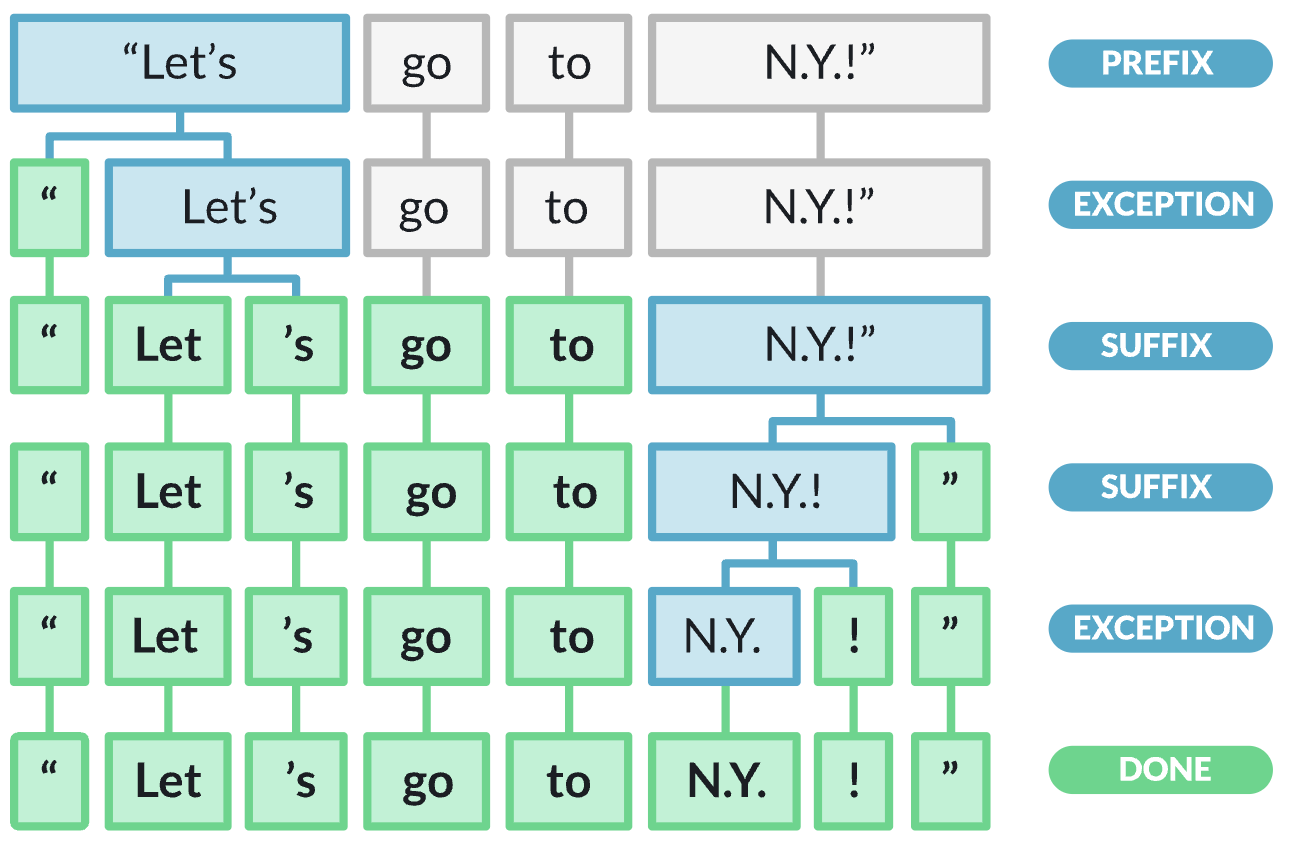
\includegraphics[width=0.8\linewidth]{cs4248-str-spacy.png}
    \item Sequential labeling and extract based on same label.
    \item Language issues: e.g. Chinese is not space-separated, but longest prefix matching works well.
  \end{itemize}

  \subsubsection{Sub-word based tokenization}
  \begin{itemize}
    \item Why: OOV and rare words are problematic. We want to split them into known tokens.
    \item \textbf{BPE token learner}:
    \item \begin{enumerate}
      \item Marks end of word with "\_".
      \item Find the 2 tokens most frequently adjacent to each other.
      \item Merge them.
      \item Repeat until $k$ merges have been done.
    \end{enumerate}
    \item \textbf{WordPiece}:
    \item \begin{itemize}
      \item Marks continuation of a word with "\_". (e.g. n \_e \_w \_e \_s \_t)
      \item Fundamental difference: find the 2 tokens \textcolor{red}{most likely} adjacent to each other.
      \item Likelihood: $\frac{P(t_1, t_2)}{P(t_1)P(t_2)} = \frac{P(t_2|t_1)}{P(t_2)} \propto \frac{count(t_1, t_2)}{count(t_1)\cdot count(t_2)}$
      \item 
    \end{itemize}
  \end{itemize}

  \subsubsection{Normalization}
  \begin{itemize}
    \item Goal: convert to a canonical form. e.g. U.S.A \textrightarrow \ USA.
    \item Opposite: asymmetric expansion
    \item \textbf{Case folding}: When not to fold? NER, machine translation
    \item \textbf{Stemming}: Reduce words to their stem by crudely chopping affixes.
    \item \textbf{Lemmatization}: Reduce inflections to base form, differentiating the word forms (requires POS tags).
  \end{itemize}

  \subsubsection{Sentence segmentation}
  \begin{itemize}
    \item Binary classification of each period (e.g. with a decision tree)
    \item Other possible features: length of words before/after the period, distance to the next punctuation mark, probabilities derived from a dataset, \dots
  \end{itemize}
  
  \section{3 - n-Gram}
  \subsection{Language models}
  \begin{enumerate}
    \item Application of Chain Rule: $P(w_1, \dots, w_i) = P(w_1) \cdot P(w_2|w_1) \cdot \dots \cdot P(w_i|w_{1:i-1})$
    \item MLE: $P(w_i|w_{1:i-1}) = \frac{count(w_{1:i-1}w_i)}{count(w_{1:i-1})}$
  \end{enumerate}
  \begin{itemize}
    \item Problems: very long sequences \textrightarrow\ $count(\cdot) = 0$
  \end{itemize}
  
  \subsubsection{Markov assumption: n-Gram models}
  \begin{itemize}
    \item Use log for small products.
    \item Handle OOV: special token, subword tokenization or \textbf{smoothing}.
  \end{itemize}

  \subsection{Smoothing}
  \subsubsection{Laplace smoothing}
  \begin{itemize}
    \item Add 1
    \item $P_{Laplace}(w_n|w_{1:n-1}) = \frac{count(w_{1:n-1}w_n) + 1}{count(w_{1:n-1}) + |V|}$
    \item Problem: some non-zero probabilities changes a lot.
    \item $count^*(w_{n-1}w_n) = (count(w_{n-1}w_n) + 1)\cdot\frac{count(w_{n-1})}{count(w_{n-1}) + |V|}$
    \item $d_c = \frac{count^*}{count}$
  \end{itemize}
  \subsubsection{Backoff \& interpolation}
  \begin{itemize}
    \item Backoff: If trigram P not available, use bigram P.
    \item Interpolation: Estimate trigram P as a weighted sum of trigram P, bigram P and unigram P, with learnable weights conditioned on the context.
    \item Learning the weights: train-test split the corpus and find the weights that maximizes over the test corpus.
  \end{itemize}

  \subsubsection{Kneser-Ney smoothing (bigram only)}
  $P_{KN}(w_n|w_{n-1}) = \frac{\max[count(w_{n-1}w_n)-d, 0]}{count(w_{n-1})} + \lambda(w_{n-1})P_{KN}(w_n)$
  \begin{itemize}
    \item Absolute discounting: removes fixed $d$ from bigram counts (intuition: big counts are hardly affected and small counts are not useful to begin with). $d$ set to about 0.75.
    \item Interpolation with a twist:
    \item \begin{itemize}
      \item $P_{KN}(w)$: How likely is $w$ to appear as a novel continuation?
      \item $P_{KN}(w) = \frac{\text{\# words }w'\text{that form an existing bigram }w'w}{\text{total number of existing bigrams}}$
    \end{itemize}
    \item Normalizing factor $\lambda(w_{n-1}) = \frac{d}{count(w_{n-1})}\cdot|\{w':count(w_{n-1}w')>0\}|$ (\# words that can follow)
  \end{itemize}

  \subsection{Evaluating language models}
  \begin{itemize}
    \item Extrinsic: Use downstream task.
    \item Intrinsic: Evaluate each LM on a test corpus.
    \item \begin{enumerate}
      \item Train LM on a training corpus (80\%)
      \item Tune parameters with a development corpus (10\%)
      \item Evaluate on test corpus (10\%)
    \end{enumerate}
  \end{itemize}
  \subsubsection{Perplexity}
  \begin{itemize}
    \item $PP(W) = \sqrt[N]{\frac{1}{P(w_1, w_2, \dots, w_N)}}$
    \item $\ln PP(W) = -\frac{1}{N}P(w_1,w_2,\dots,w_N)$
  \end{itemize}

  \section{4 - Text Classification}
  \subsection{Naive Bayes}
  \begin{itemize}
    \item \textbf{BoW representation}: affected by tokenization and normalization.
    \item Independent assumption: $P(y|w_1, w_2, \dots,w_n) \propto P(w_1|y)P(w_2|y)\dots P(w_n|y)P(y)=P(y)\prod_{i=1}^{n}P(w_i|y)$
    \item $P(y)\approx \frac{N_y}{N}$ (no. of documents of class y / total no. of documents)
    \item $P(w_i|y) \approx \frac{count(w_i, y)}{\sum_{w\in V}count(w, y)}$ (total occurrences of w in all documents of class y / total words in documents of class y)
    \item Arithmetic underflow: use log
    \item OOV: Add-k smoothing: $\hat{P}(w_i|y) = \frac{count(w_i, y) + k}{\sum_{w\in V}count(w, y) + k|V|}$, $\hat{P}(y) = \frac{N_y + k}{N + k|Y|}$
    \item NB vs LM:
    \item \begin{itemize}
      \item NB is unigram model.
      \item NB treats each class like a separate language model.
    \end{itemize}
    \item Limitation: BoW cannot handle negation (with only addition of word "not"). Mitigation: Add "not\_" to all the words between negation word and next punctuation mark.
  \end{itemize}

  \subsection{Evaluation of classifiers}
  \begin{itemize}
    \item Accuracy = (TP + TN) / (all 4)
    \item Precision = TP / (TP + FP)
    \item Recall = TP / (TP + FN)
    \item F1 = $2\cdot\frac{Precision\cdot Recall}{Precision + Recall}$
    \item Why harmonic mean? Imbalanced dataset.
    \item Micro averaging: average the raw values across confusion matrices. (Favors bigger classes)
    \item Macro averaging: average the F1s across each confusion matrix.
    \item A 2-class classifier and a 10-class classifier both have same F1. The 10-class classifier probably does better. Reason: Consider random guessing, 2-class \textrightarrow 50\% correctness, 10-class \textrightarrow 10\% correctness.
  \end{itemize}

  \subsection{Vector space model}
  \begin{itemize}
    \item DTM with binary weights: $w_{t,d} = 1$: document $d$ contains term $t$.
    \item DTM with term frequencies: $tf_{t,d}$ = \# occurrences of term $t$ in document $d$.
    \item \begin{itemize}
      \item Relative importance: $w_{t,d} = 1 + \log_{10}tf_{t,d}$
      \item Cross-document importance: $idf_t = \log_{10}\frac{|D|}{df_t}$, $df_t$: \# documents containing t.
      \item \textbf{Together}: $w_{t,d} = (1 + \log_{10}tf_{t,d})\cdot \log_{10}\frac{|D|}{df_t}$
    \end{itemize}
  \end{itemize}
  \subsubsection{Document similarity}
  \begin{itemize}
    \item Approach 1: dot product
    \item \begin{itemize}
      \item Overly favors frequent words.
    \end{itemize}
    \item Approach 2: cosine similarity
    \item \begin{itemize}
      \item $\frac{v\cdot w}{|v| \cdot |w|}$
      \item Value is always +ve for document vectors since vector entries are all +ve.
    \end{itemize}
  \end{itemize}

  \section{5 - Connectionist ML}
  \subsection{Generative vs discriminative classifiers}
  \begin{itemize}
    \item Generative: $\hat{y} = \argmax_{y\in Y}P(x|y)P(y)$
    \item Discriminative: $\hat{y} = \argmax_{y\in Y}P(y|x)$
  \end{itemize}
  \subsection{Logistic regression}
  \begin{itemize}
    \item $\hat{y} = \frac{1}{1 + e^{-\theta^\top x}}$
  \end{itemize}
  \subsubsection{Loss Function}
  \begin{itemize}
    \item $L_{CE}(\hat{y}, y) = -[y\log\hat{y} + (1-y)\log(1-\hat{y})]$
    \item Given $m$ samples, $L_{CE} = \frac{1}{m}\sum_j L_{CE}(\hat{y}_j, y_j)$.
    \item 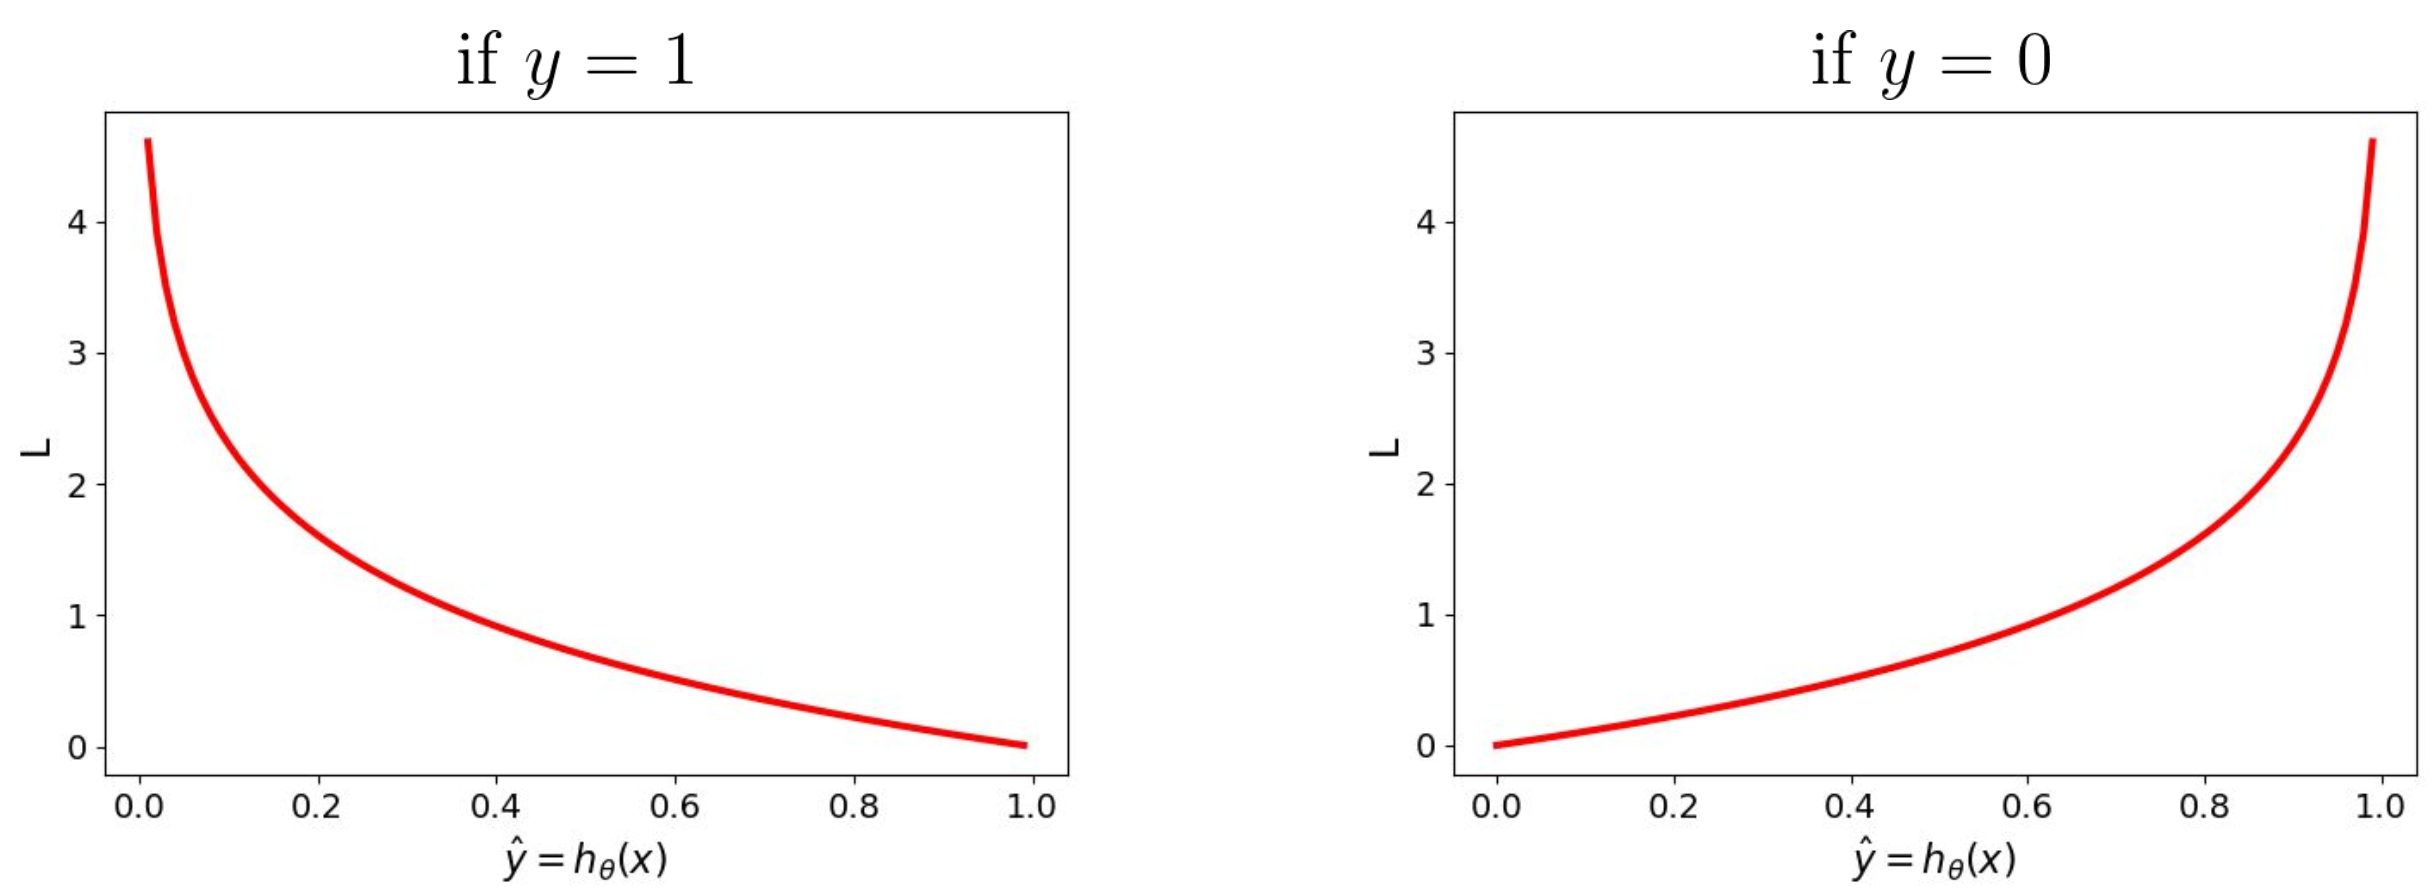
\includegraphics[width=\linewidth]{cs4248-ml-crossentropy.png}
    \item Generalized for MLR: $L_{CE}(\hat{y}, y) = -\sum_{i=1}^{C}y_i\log(\hat{y_i})$, $y_i=1$ for the correct class, 0 otherwise.
  \end{itemize}
  \subsubsection{Gradient descent}
  \begin{itemize}
    \item $\frac{\partial L_{CE}}{\partial \theta_i} = \frac{1}{m}\sum_{j=1}^{m}[\sigma(\theta^\top x^{(j)}) - y^{(j)}]x_i^{(j)}$, $\frac{\partial L_{CE}}{\partial \theta} = \frac{1}{m}X^\top[\sigma(X\theta) - y]$
  \end{itemize}
  \subsubsection{Regularization}
  \begin{itemize}
    \item L2 ("Ridge"): $L_{CE} = \dots + \lambda\sum_{i=1}^{n}\theta_i^2$
    \item L1: $L_{CE} = \dots + \lambda\sum_{i=1}^{n}|\theta_i|$
    \item Regularization definitely increases the training loss, in the hope that testing loss will be lower.
  \end{itemize}

  \subsection{Neural networks}
  \subsubsection{The XOR problem}
  \begin{itemize}
    \item 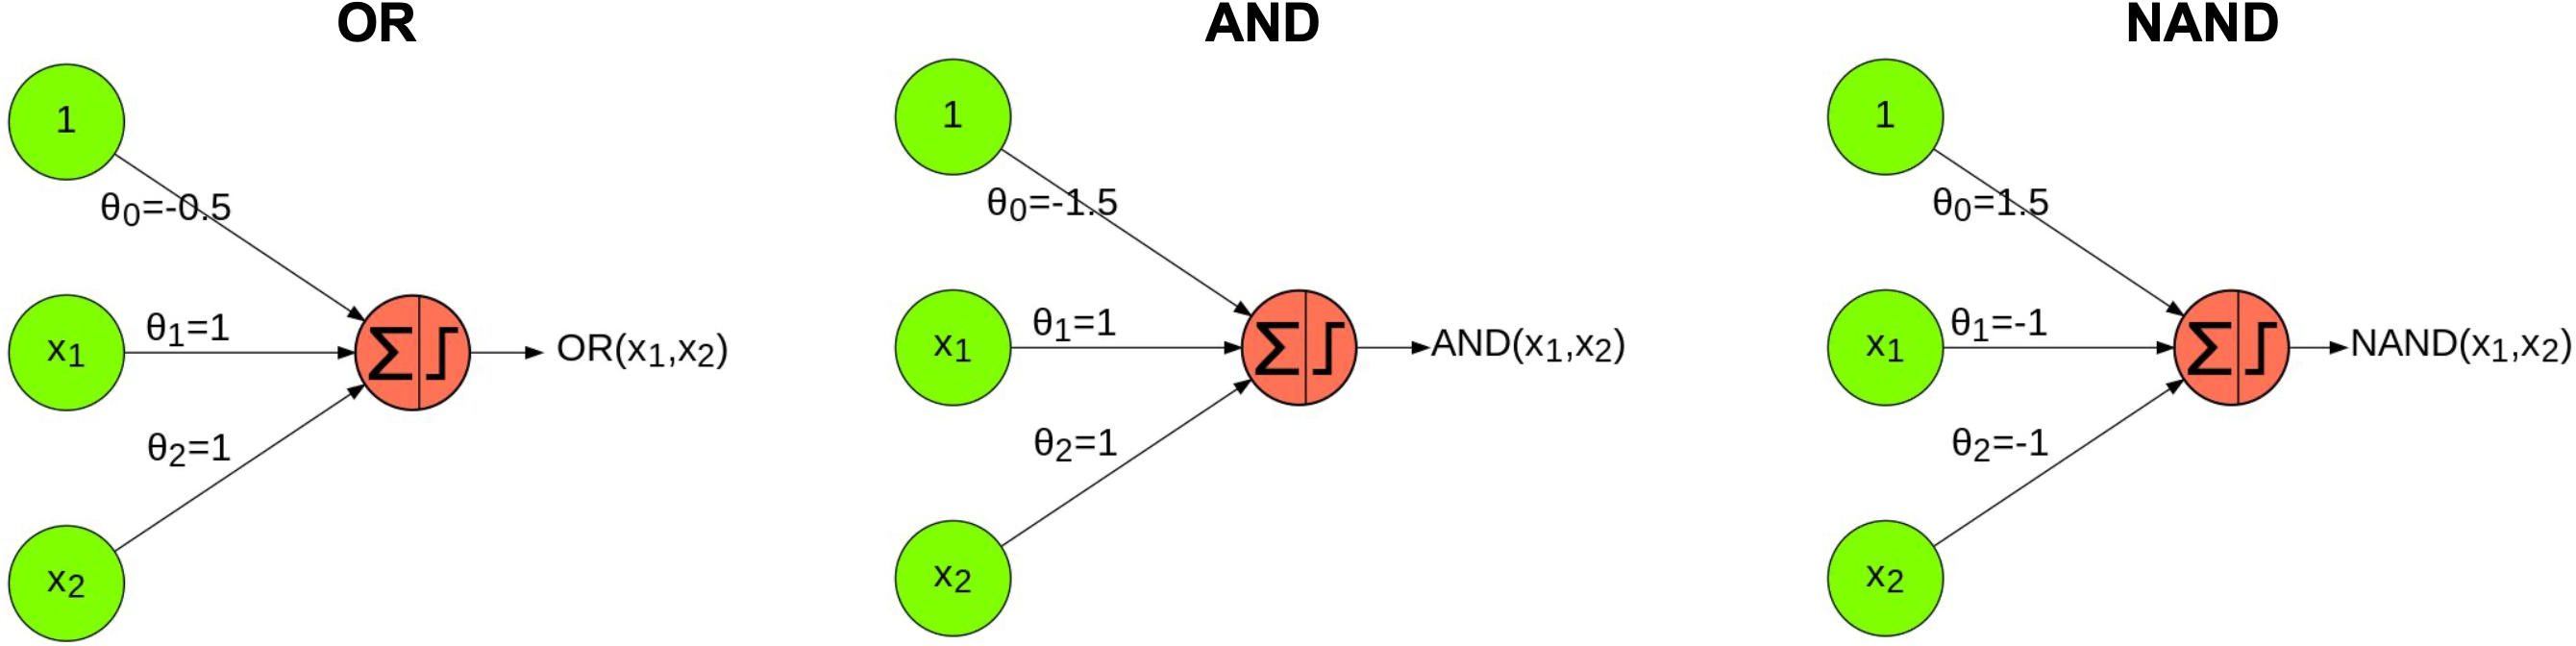
\includegraphics[width=\linewidth]{cs4248-ml-commongates.png}
    \item Observation: (OR) AND (NAND) = XOR
    \item 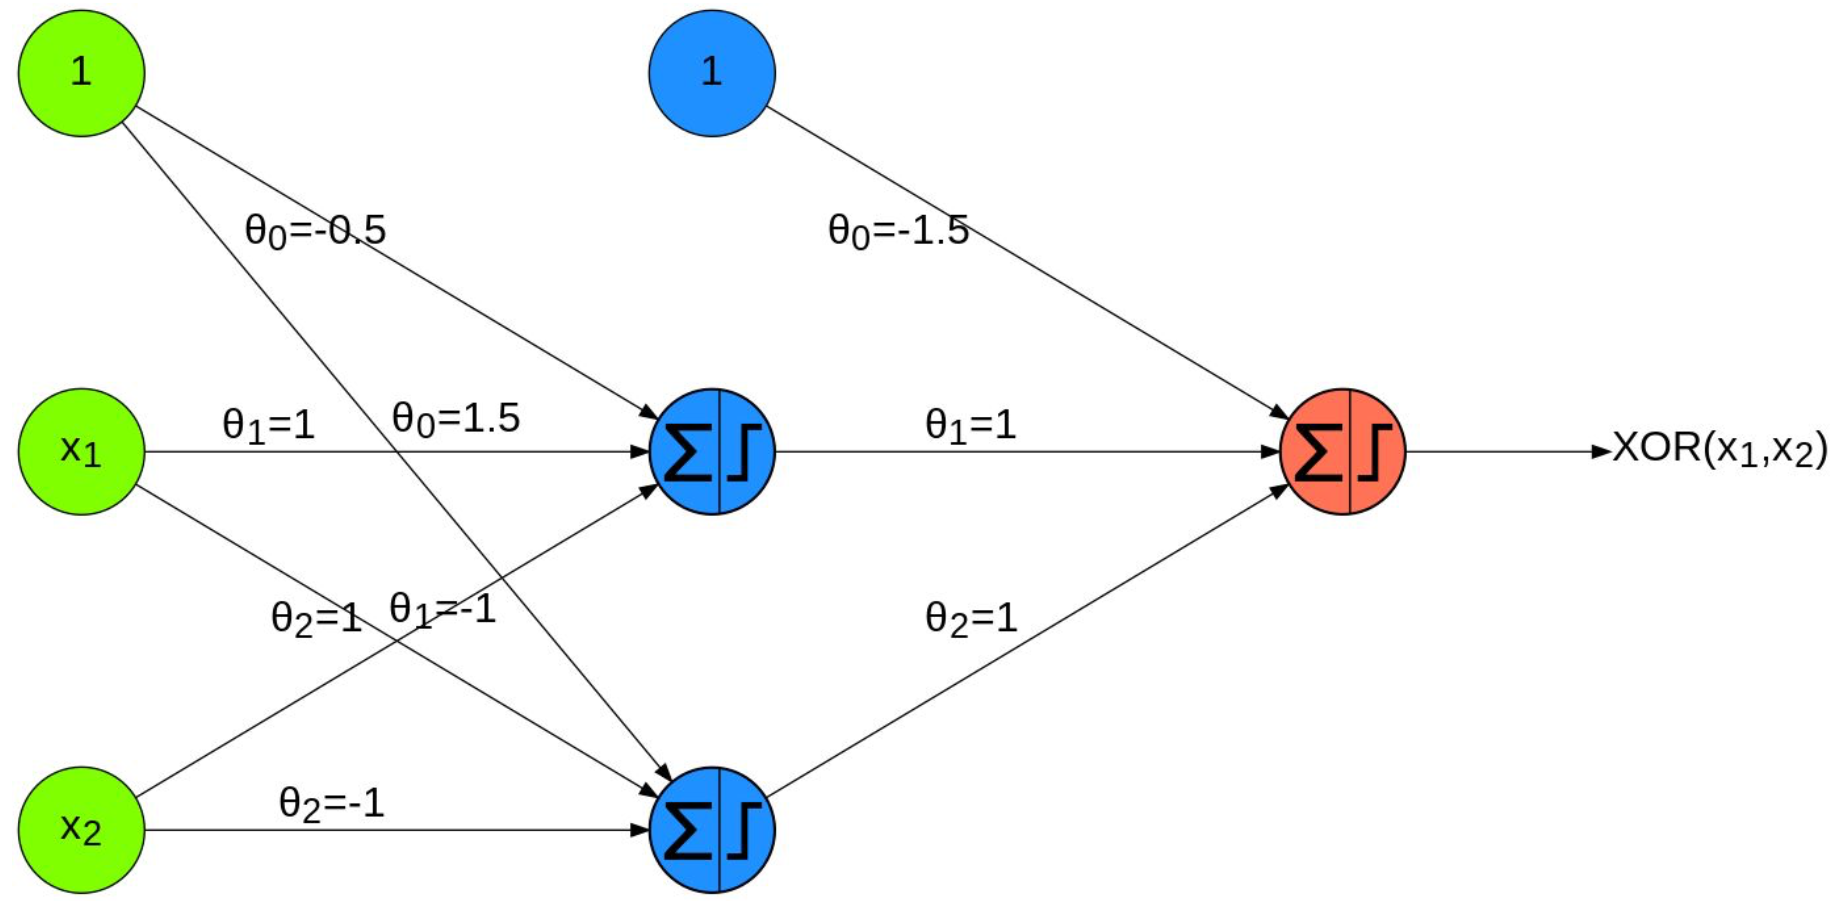
\includegraphics[width=0.8\linewidth]{cs4248-ml-xor.png}
  \end{itemize}
  \subsubsection{NN}
  \begin{itemize}
    \item 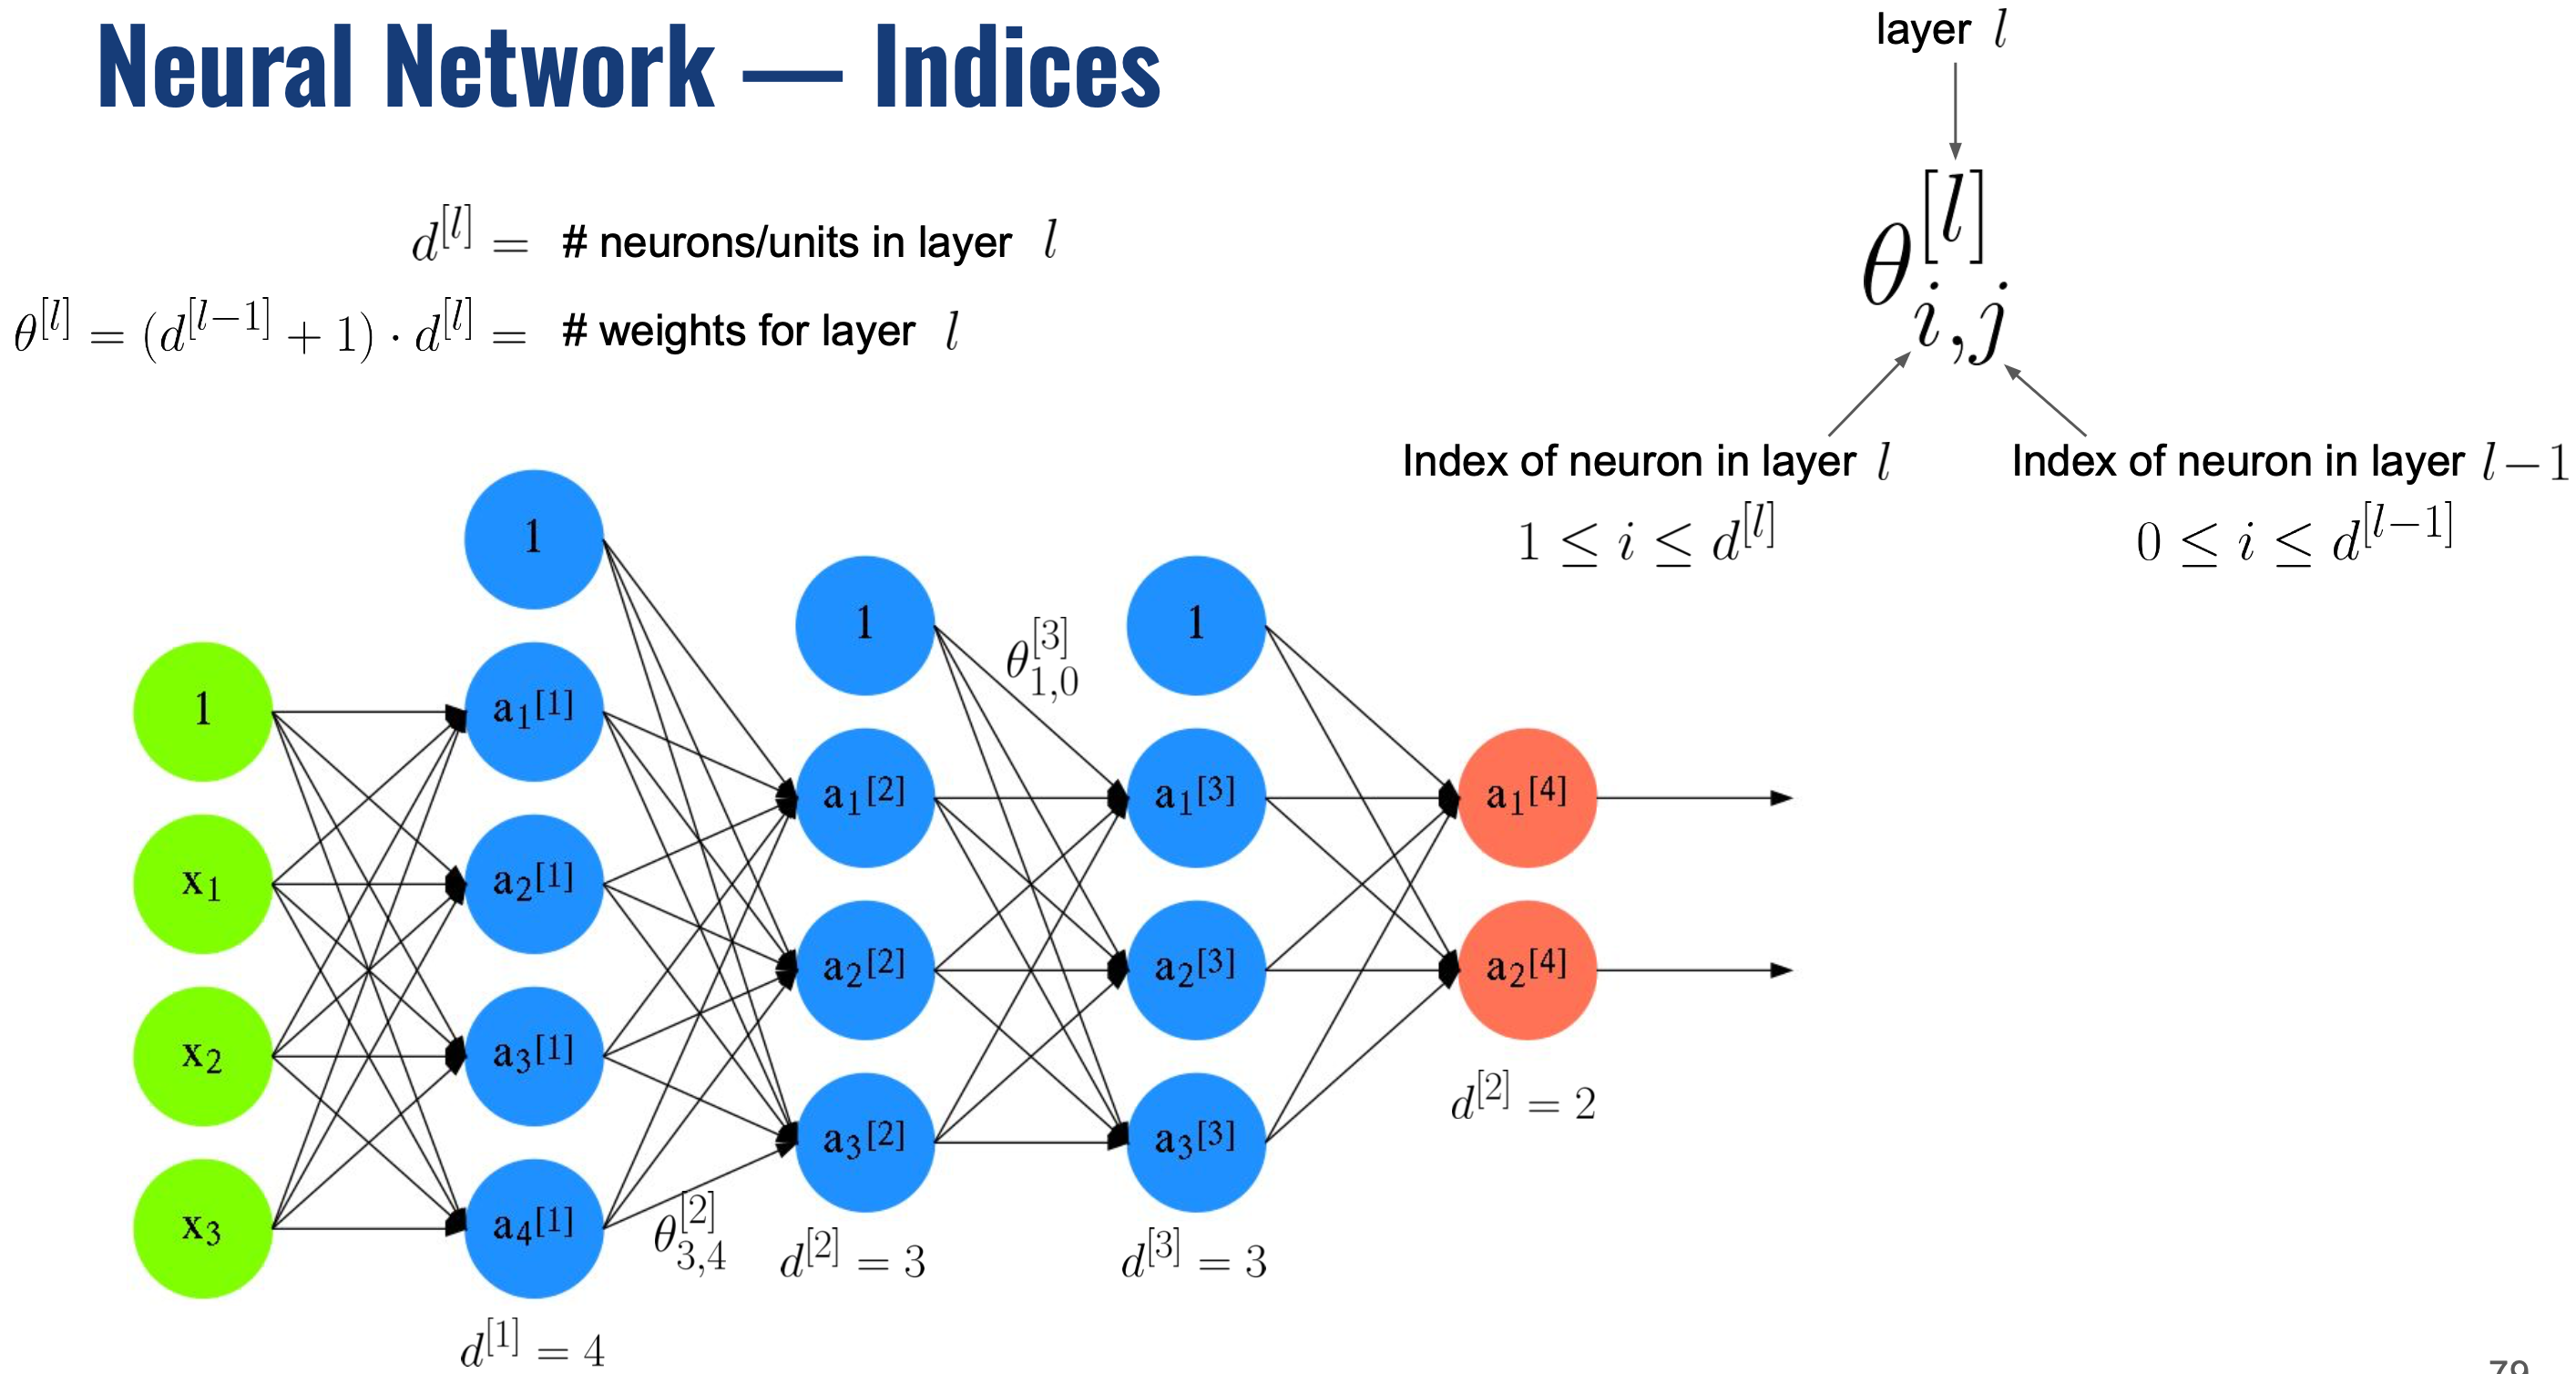
\includegraphics[width=\linewidth]{cs4248-ml-neural.png}
    \item \textbf{Activations}:
    \item \begin{itemize}
      \item Activations for hidden layers: non-linear
      \item Activations for output layers: linear for regression, sigmoid for classification.
    \end{itemize}
  \end{itemize}
  \pagebreak

  \section{6 - Word Embeddings and NLP Ethics}
  \subsection{Word Embeddings}
  \subsubsection{Symbolic Representations}
  \begin{itemize}
    \item \textbf{One-hot encoding}: Words as discrete symbols
    \item Limitation: No notion of similarity between words
  \end{itemize}

  \subsubsection{Sparse Word Representations}
  \begin{itemize}
    \item \textbf{Distributional Hypothesis}: Words that appear in similar \textbf{contexts} have similar meanings.
    \item Revisiting Document-Term Matrix (DTM)
    \begin{itemize}
      \item Assumption: context of $w$ = set of documents containing $w$
      \item Problem: does not capture distributional hypothesis
    \end{itemize}
    \item \textbf{Term-Context Matrix (TCM)}
    \item 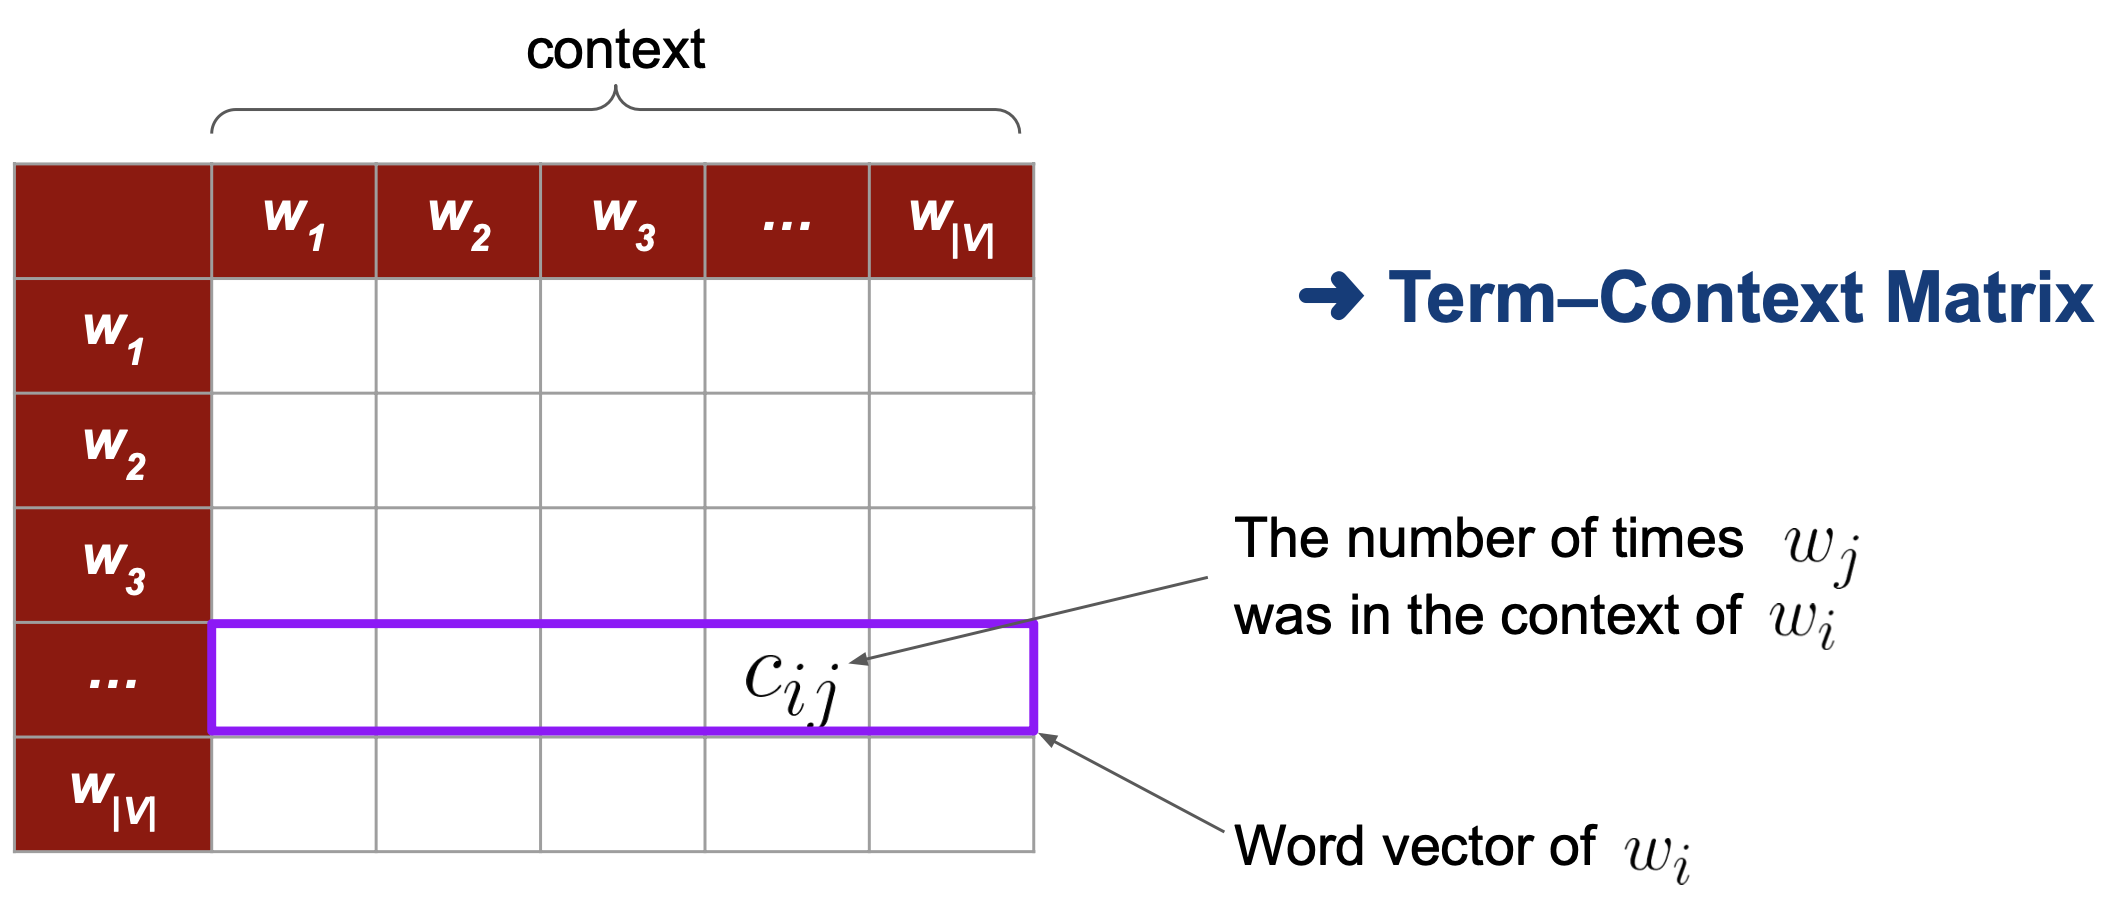
\includegraphics[width=\linewidth]{cs4248-term-context-matrix.png}
    \begin{itemize}
      \item Problem: skewed towards high-frequency words
      \item Alternative: Pointwise Mutual Information (PMI): $\text{PMI}(w_i, w_j) = \log \frac{P(w_i, w_j)}{P(w_i)P(w_j)}$
      \item Positive PMI (PPMI): $\text{PPMI}(w_i, w_j) = \max(\text{PMI}(w_i, w_j), 0)$
      \item 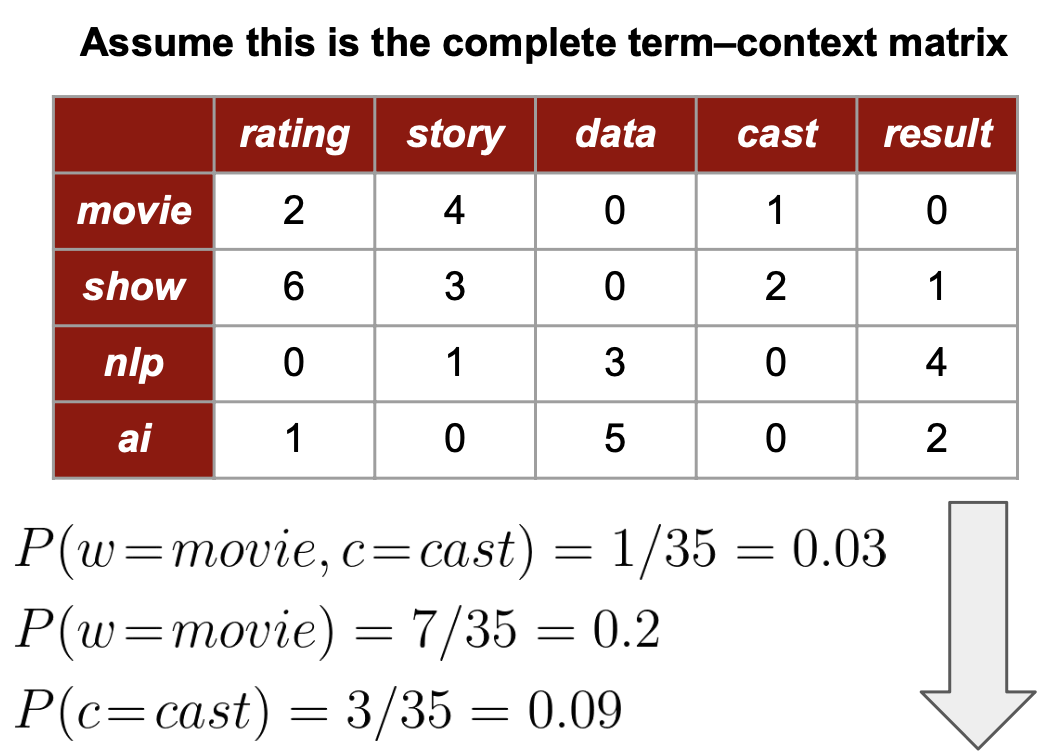
\includegraphics[width=0.8\linewidth]{cs4248-PPMI-matrix.png}
      \item Rare words: Raise context probabilities/Laplace Smoothing
      \item Sparsity: Very sparse
    \end{itemize}
  \end{itemize}  

  \subsubsection{Dense Word Representations}
  \begin{itemize}
    \item Basic idea: Learn a dense vector for each word, whose dimensions are "shared properties" of all the words.
    \item \textbf{Word2Vec}
    \begin{itemize}
      \item 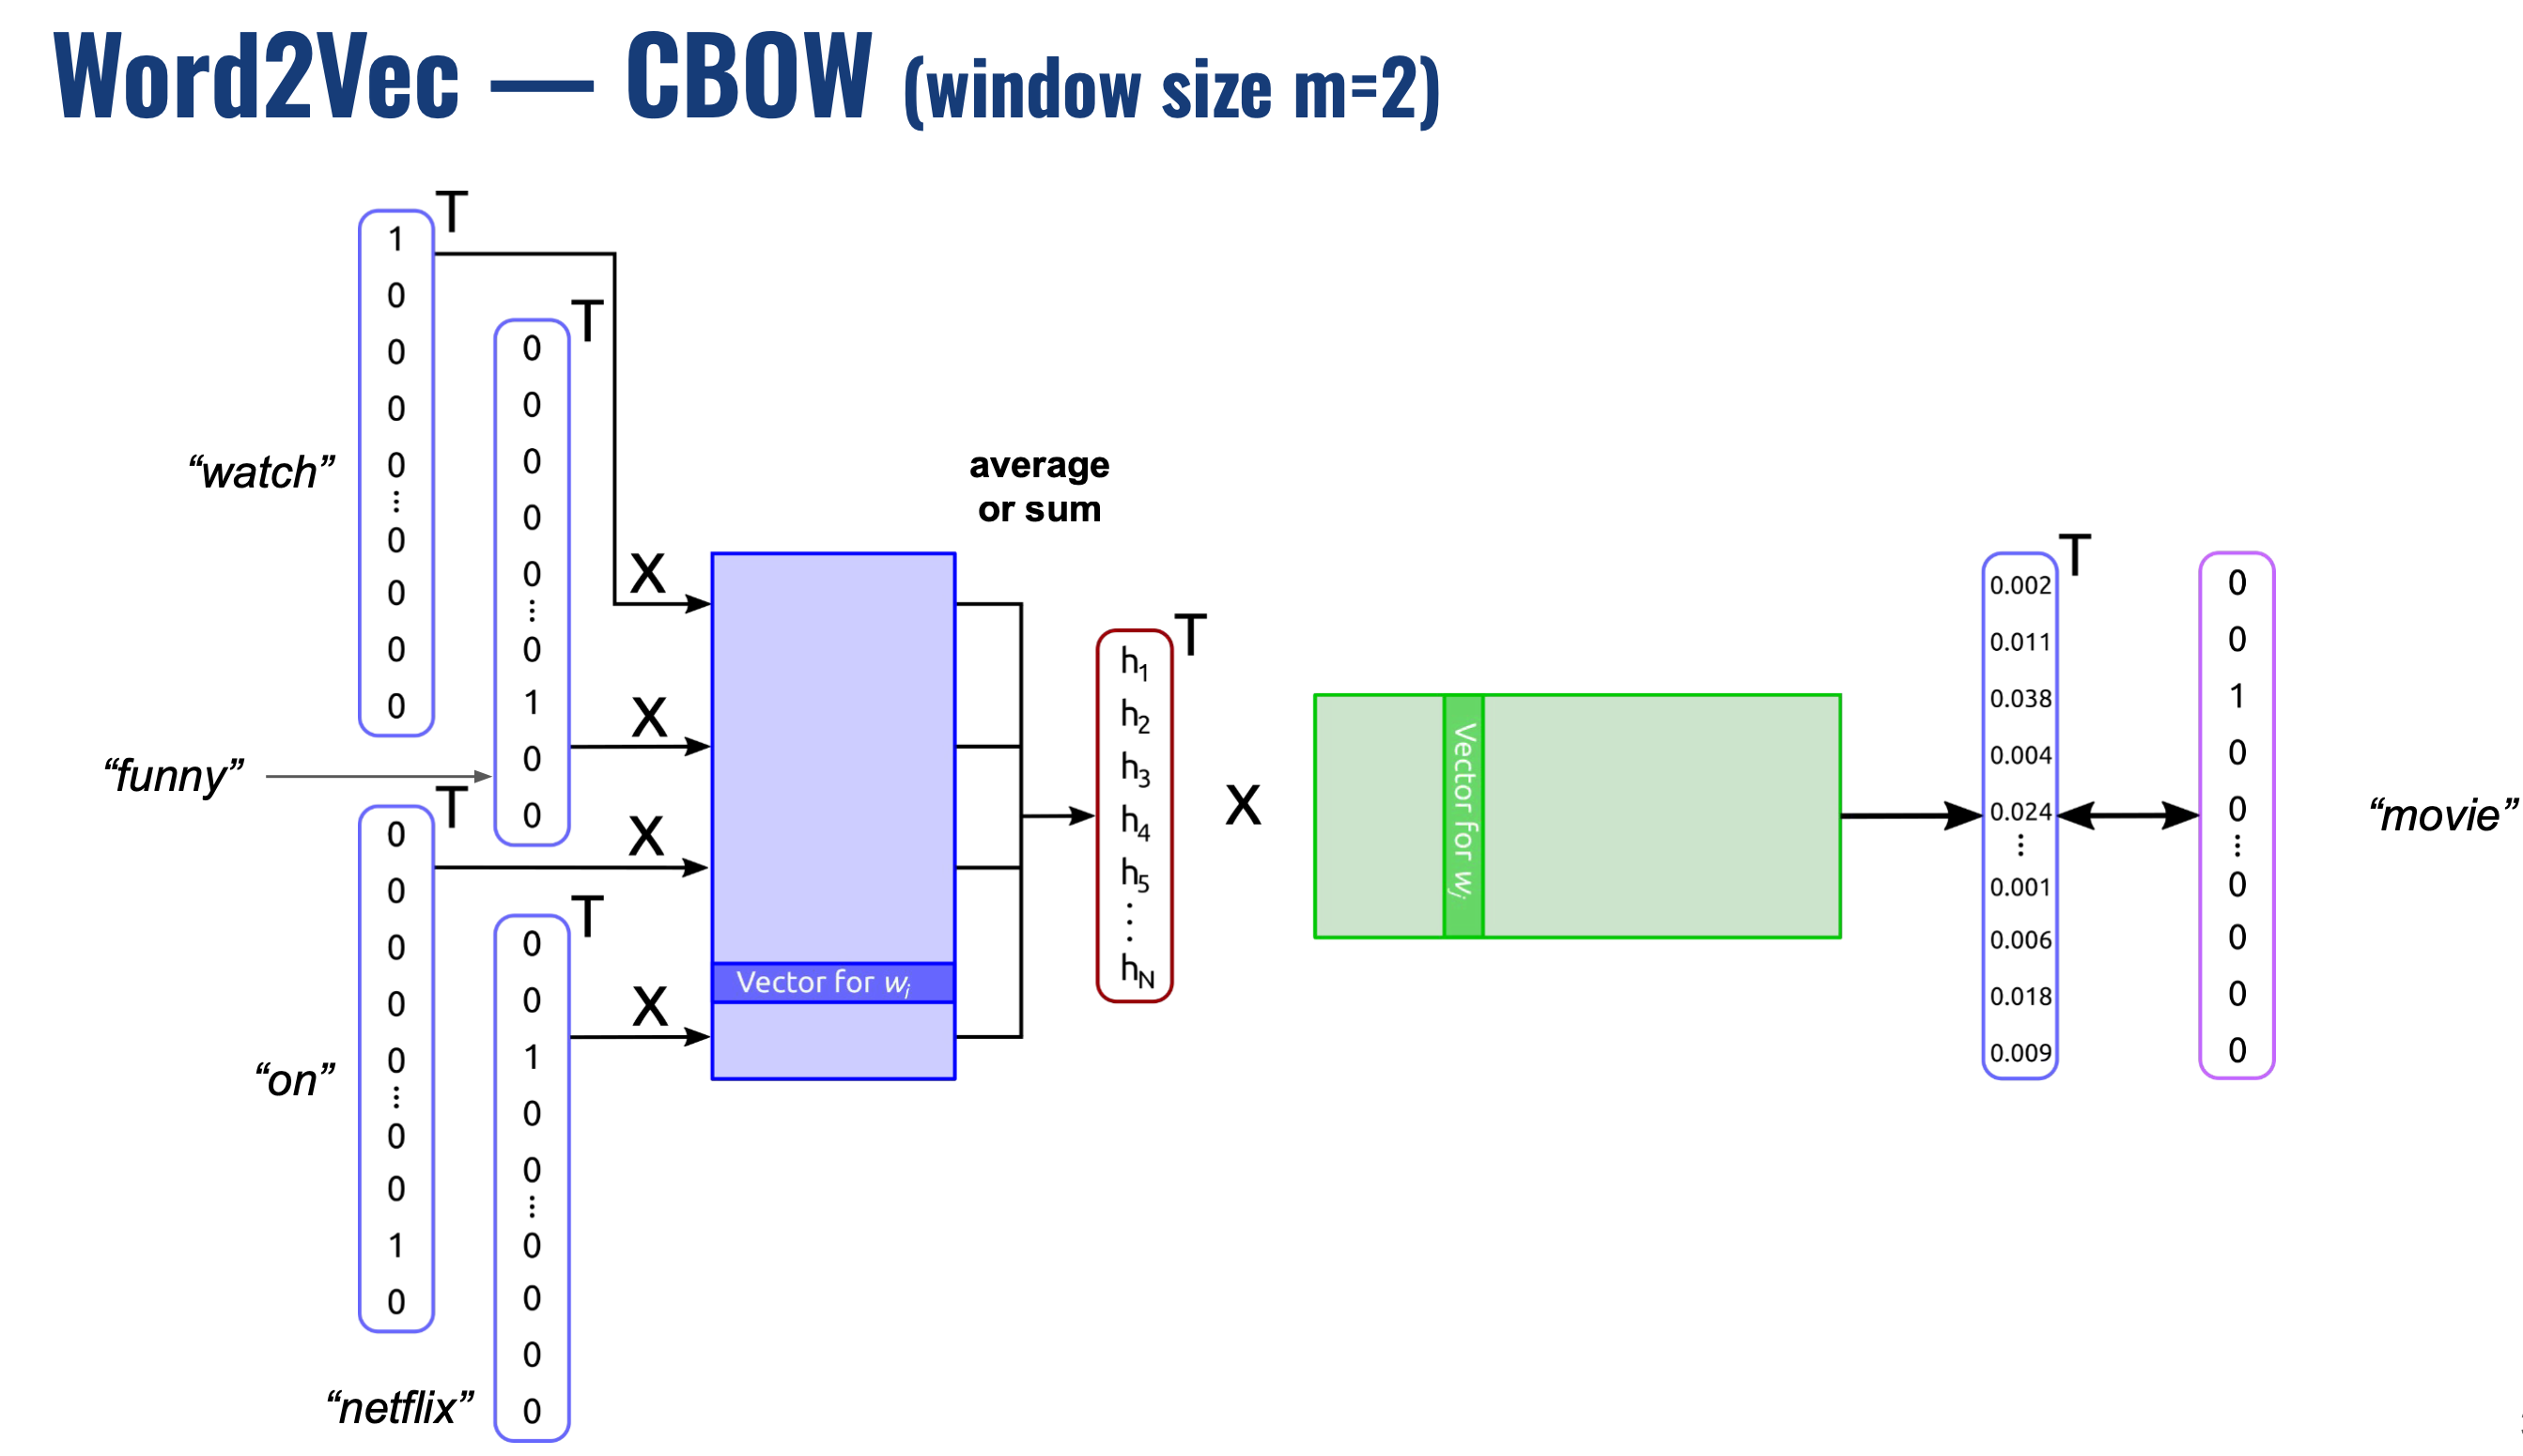
\includegraphics[width=\linewidth]{cs4248-word2vec-cbow.png}
      \item 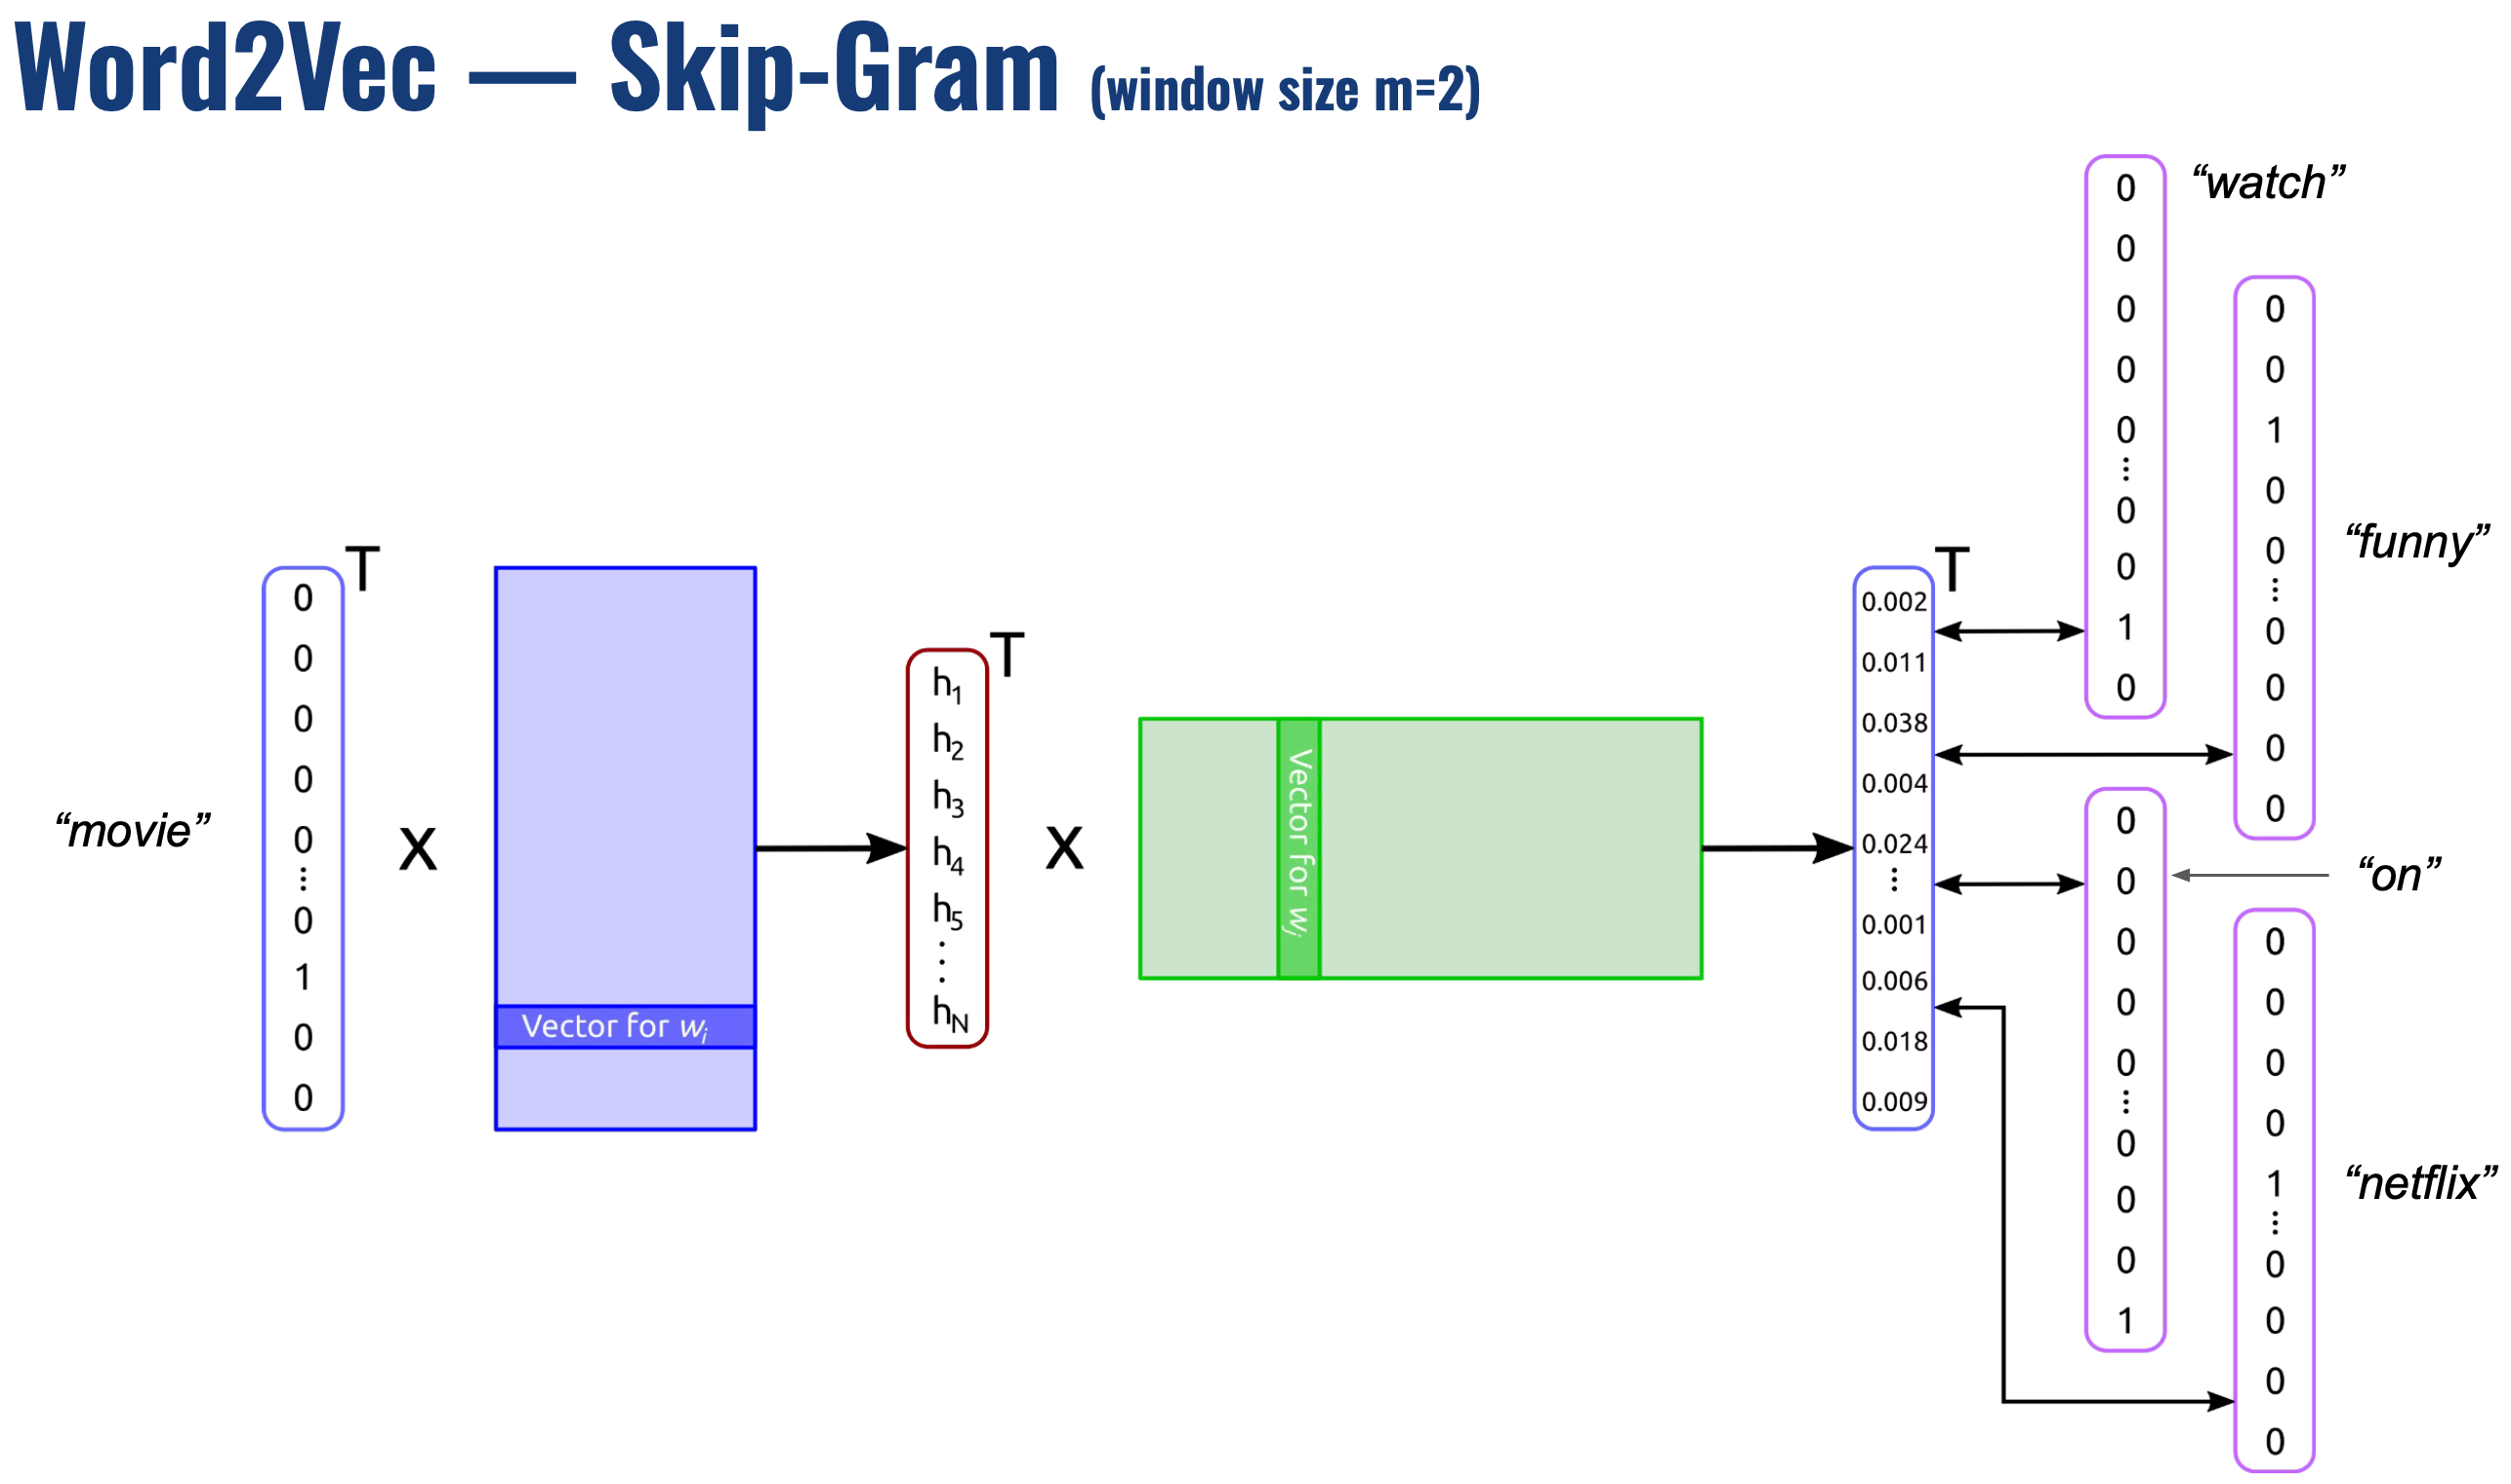
\includegraphics[width=\linewidth]{cs4248-word2vec-skipgram.png}
      \item Goal of training (CBOW): $L = -\log P(w_c|w_{c-m},\dots,w_{c-1},w_{c+1},\dots,w_{c+m})
          = -\log P(u_c|\tilde{v}), \tilde{v} = \sum_{-m\leq j \leq m, j\neq 0} v_{c+j}$
        $P(u_c|\tilde{v}) = \frac{\exp(u_c^\top\cdot\tilde{v})}{\sum_{j=1}^{|V|}\exp(u_j^\top\cdot\tilde{v})}$
      \item Goal of training (Skip-Gram): $\Pr(u_{c+j}|v_c) = \frac{\exp(u_{c+j}^\mathsf{T}\cdot v_c)}{\sum_{j=1}^{|V|}\exp(u_j^\mathsf{T}\cdot v_c)}$, "next-word prediction" task.
      \item By-product: Vectors of words with similar contexts are close.
      \item Word vectors: $u$ or $v$ or an average of both.
      \item 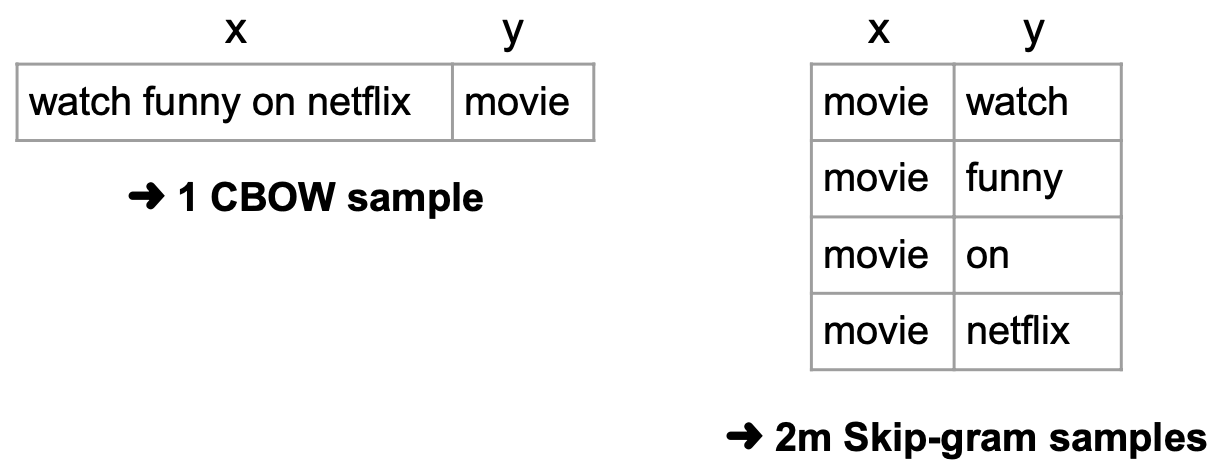
\includegraphics[width=\linewidth]{cs4248-word2vec-training.png}
    
      \item \textbf{Skip-Gram with Negative Sampling (SGNS)}
      \begin{enumerate}
        \item Produce $2m$ positive samples from the input string.
        \item Produce $2mk$ negative samples from $V$.
        \begin{itemize}
          \item Penalize common words: $P_\alpha(w_i) = \frac{Count(w_i)^\alpha}{\sum_{j=1}^{|V|}Count(w_j)^\alpha}, 0<\alpha\leq1$
        \end{itemize}
        \item $P(+|c,m) = \frac{1}{1+\exp(-u_{m}^\mathsf{T}v_c)} = \sigma(u_{m}^\mathsf{T}v_c), P(-|c,m) = 1 - P(+|c,m)$
        \item $L = -\left[\sum_{(c,m)\in B_+}\log\sigma(u_{m}^\mathsf{T}v_c) + \sum_{(c,m)\in B_-}\log\sigma(-u_{m}^\mathsf{T}v_c)\right]$
      \end{enumerate}
      \begin{itemize}
        \item Hyperparameters:
        \begin{itemize}
          \item Sampling method to generate negative samples.
          \item Number of negative samples $k$ (5-20 for small text, 2-5 for large text).
        \end{itemize}
      \end{itemize}

      \item Limitations:
      \item \begin{itemize}
        \item Unable to represent phrases.
        \item Unable to handle polysemy (multiple meanings) and part of speech.
      \end{itemize}

      \item Practical considerations:
      \item \begin{itemize}
        \item Skip-gram slower, better for infrequent words. CBOW faster.
        \item Hierarchical softmax better for infrequent words, negative sampling better for frequent words, better with low dimensional vectors.
      \end{itemize}
    \end{itemize}
  \end{itemize}

  \subsection{NLP Ethics}
  \subsubsection{Biases}
  \begin{itemize}
    \item Bias in word embeddings: e.g. $v(programmer) - v(man) + v(woman) \approx v(homemaker)$
    \item Bias in sentiment analysis: e.g. different sentiment scores for different cuisine.
  \end{itemize}
  \subsubsection{Towards debiasing}
  \begin{itemize}
    \item \textbf{Measuring bias}: e.g. find pairs of (x, y) that minimize $cosine(v(she) - v(he), v(x) - v(y))$.
    \item \textbf{Identify gender subspace}: Pick top pairs of gender words, compute difference vectors, use top PCs from PCA as gender subspace.
    \item Train binary classifier to identify gender-neural/specific words.
    \item Embedding transformation:
    \item 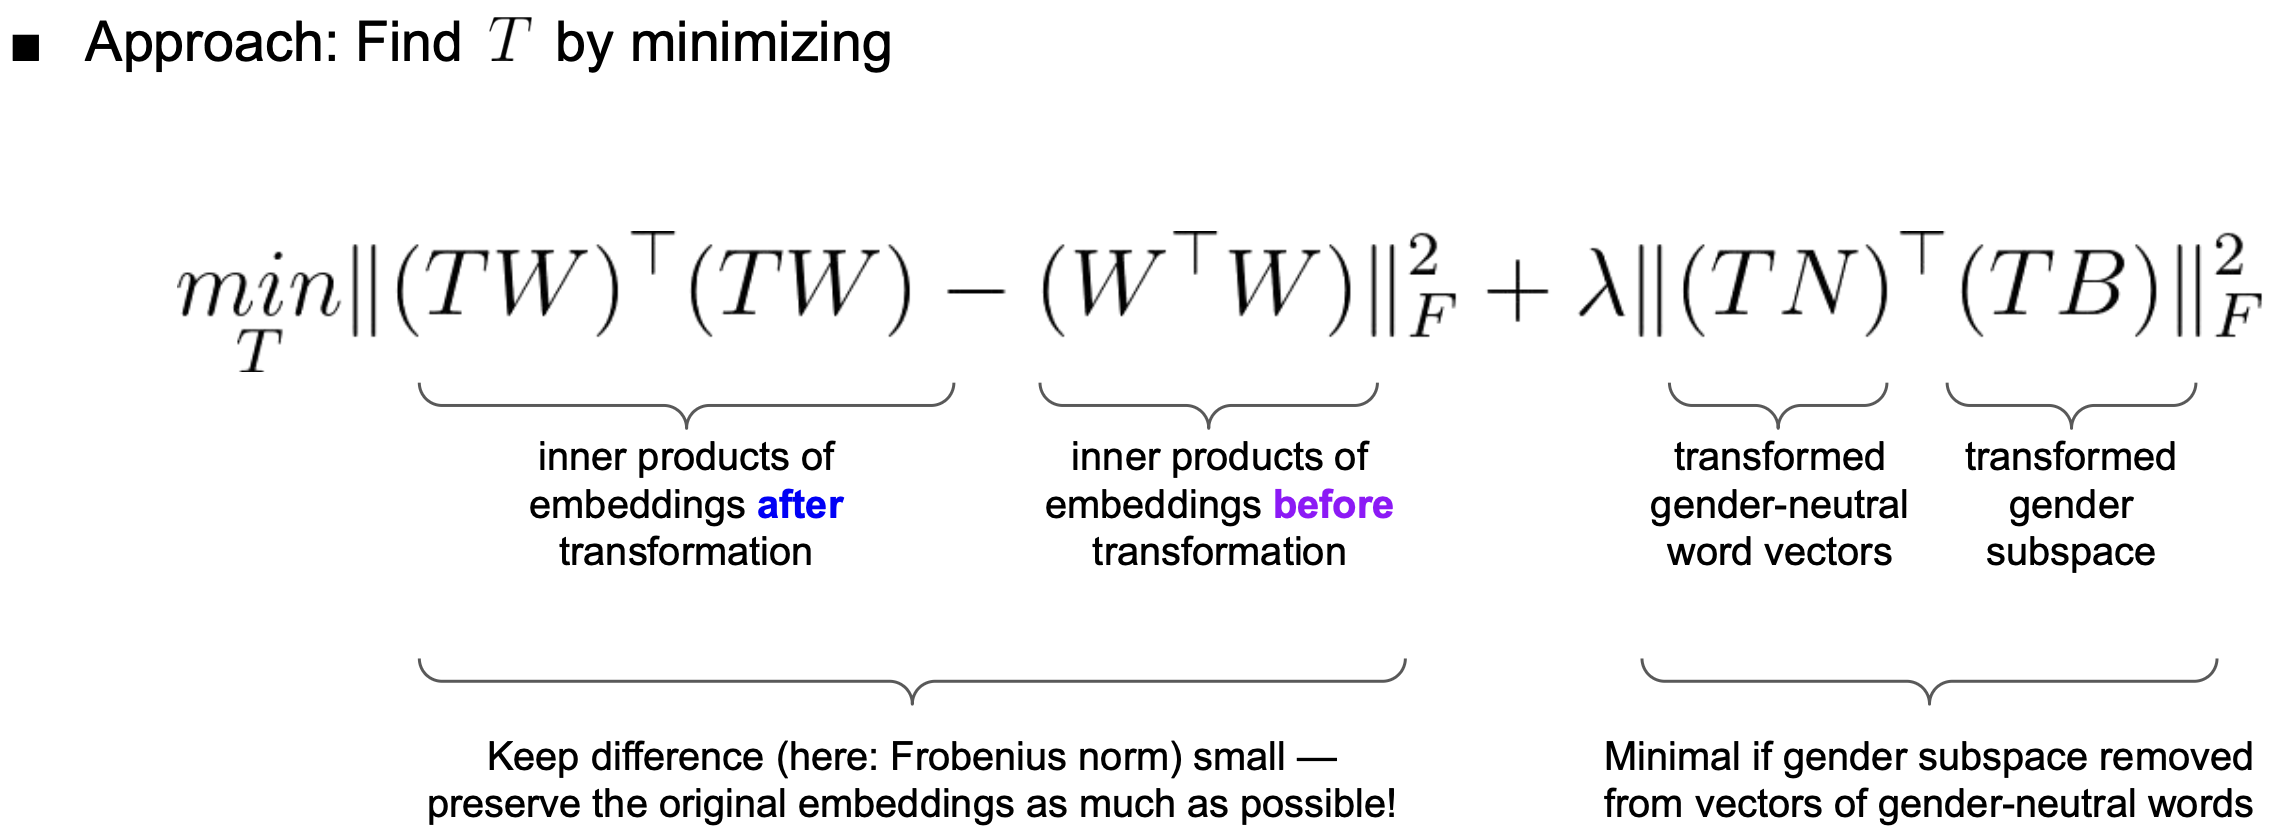
\includegraphics[width=\linewidth]{cs4248-ethic-trans.png}
    \item $\| A \|_F^2 = \sqrt{ \sum_{i=1}^m \sum_{j=1}^n |a_{ij}|^2 }$
    \item Generate morphological variations (grammatically incorrect) data to desensitize the model.
  \end{itemize}

  \section{7 - Sequences}
  \subsection{POS Tagging}
  \begin{itemize}
    \item Two categories:
    \begin{itemize}
      \item Closed class: small, fixed set of words (e.g. prepositions, conjunctions)
      \item Open class: large, open set of words (e.g. nouns, verbs)
    \end{itemize}
  \end{itemize}
  \subsubsection{Baseline: Label with most frequent tag}
  \begin{itemize}
    \item Limitations:
    \begin{itemize}
      \item Imbalanced: High accuracy for common unambiguous words, which are not interesting for downstream tasks.
      \item Downstream error propagation: Errors in POS tagging quickly propagate up.
    \end{itemize}
  \end{itemize}
  \subsubsection{Unsupervised Algorithms}
  \begin{itemize}
    \item Anchor words: Words with unambiguous POS tags.
  \end{itemize}
  \subsection{Supervised Algorithms: Hidden Markov Models}
  \begin{itemize}
    \item Notations:
    \begin{itemize}
      \item The HMM $\theta = (A, B, \pi)$ 
      \item Finite set of states (\textbf{POS tags}) $S = \{s_1, s_2, \ldots, s_N\}$
      \item Sequences of states $Q = q_1, q_2, \ldots, q_T, q_t \in S$
      \item Finite set of observations (\textbf{words}) $V = \{v_1, v_2, \ldots, v_M\}$
      \item Sequences of observations $O = o_1, o_2, \ldots, o_T, o_t \in V$
      \item Transition probabilities $a_{ij} = P(q_t = s_j|q_{t-1} = s_i)$
      \item Emission probabilities $b_i(o_k) = P(o_t = v_k|q_t = s_i)$
      \item Initial state probabilities $\pi_i = P(q_1 = s_i)$
    \end{itemize}
    \item Core tasks:
    \begin{itemize}
      \item Model learning: Given $Q$ and $O$, learn $A$, $B$, $\pi$.
      \item Likelihood: Given $\theta$, $Q$ and $O$, compare $P(O|Q, \theta)$.
      \item Decoding: Given $\theta$ and $O$, find $Q$.
    \end{itemize}
  \end{itemize}
  \subsubsection{Model Learning}
  \begin{itemize}
    \item $\pi_i = P(q_1 = s_i) = \frac{Count(<S>s_i)}{Count(<S>)}$
    \item $a_{ij} = P(q_t = s_j|q_{t-1} = s_i) = \frac{Count(s_i s_j)}{Count(s_i)}$
    \item $b_i(o_k) = P(o_t = v_k|q_t = s_i) = \frac{Count(v_k, s_i)}{Count(s_i)}$
  \end{itemize}
  \subsubsection{Likelihood}
  \begin{itemize}
    \item $P(O, Q|\theta) = \prod_{t=1}^T P(o_t|q_t)P(q_t|q_{t-1}), P(q_1|q_0) = P(q_1)$
  \end{itemize}
  \subsubsection{Decoding}
  \begin{itemize}
    \item Naive decoding: Enumerate all possible $Q_i$ and find $\argmax_{Q_i} P(O, Q_i|\theta)$
    \item Runtime complexity: $O(|Q|^T\cdot T)$ (T for computing joint probability)
    \item Viterbi Algorithm:
    \begin{itemize}
      \item For every state $s_j$ at time $t$, compute the probabilities of all inward paths ($O(|Q|)$) and keep the path with the highest probability.
      \item Runtime complexity: $O(|Q|^2\cdot T)$
      \item Recursion:
      \begin{itemize}
        \item $v_t(j) = \max_{i=1}^{|Q|} v_{t-1}(i)a_{ij}b_j(o_t)$
        \item $bt_t(j) = \argmax_{i=1}^{|Q|} v_{t-1}(i)a_{ij}b_j(o_t)$
      \end{itemize}
      \item Practical issue: Arithmetic underflow, use log probabilities.
    \end{itemize}
  \end{itemize}

  \section{8 - Encoder-Decoder}
  \subsection{RNNs}
  \begin{itemize}
    \item \textbf{Autoregressive Generation}: Sample further words conditioned on previous choices until: reaching a pre-determined length or an end-of-sequence token is generated.
    \item \textbf{Basic recurrent formula}: $h_t = f_\theta(h_{t-1}, x_t)$ e.g. $h_t = \tanh(\theta_{hh} h_{t-1} + \theta_{xh} x_t)$
    \item 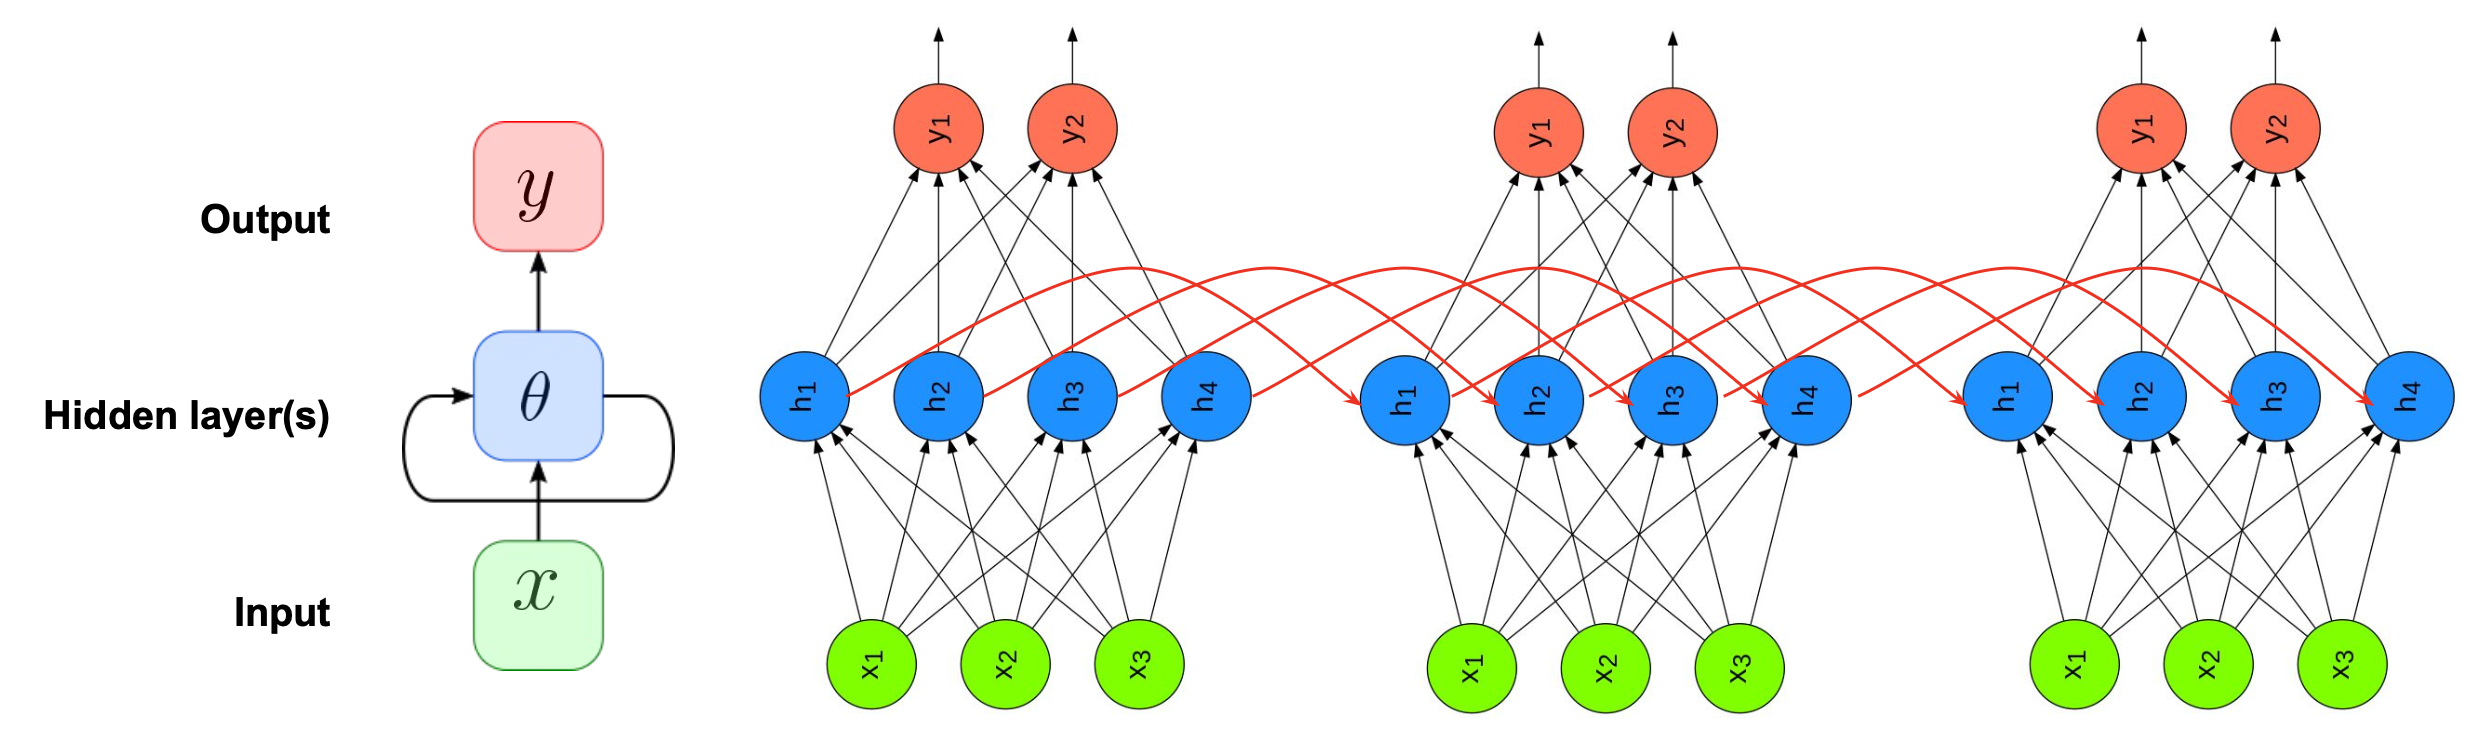
\includegraphics[width=\linewidth]{cs4248-rnn-unrolled.png}
    \item Loss calculation and backpropagation (BPTT):
    \item \textbf{Important}: parameter-tied: only one copy of $\theta_{hh}$, $\theta_{xh}$ and $\theta_{hy}$.
    \item 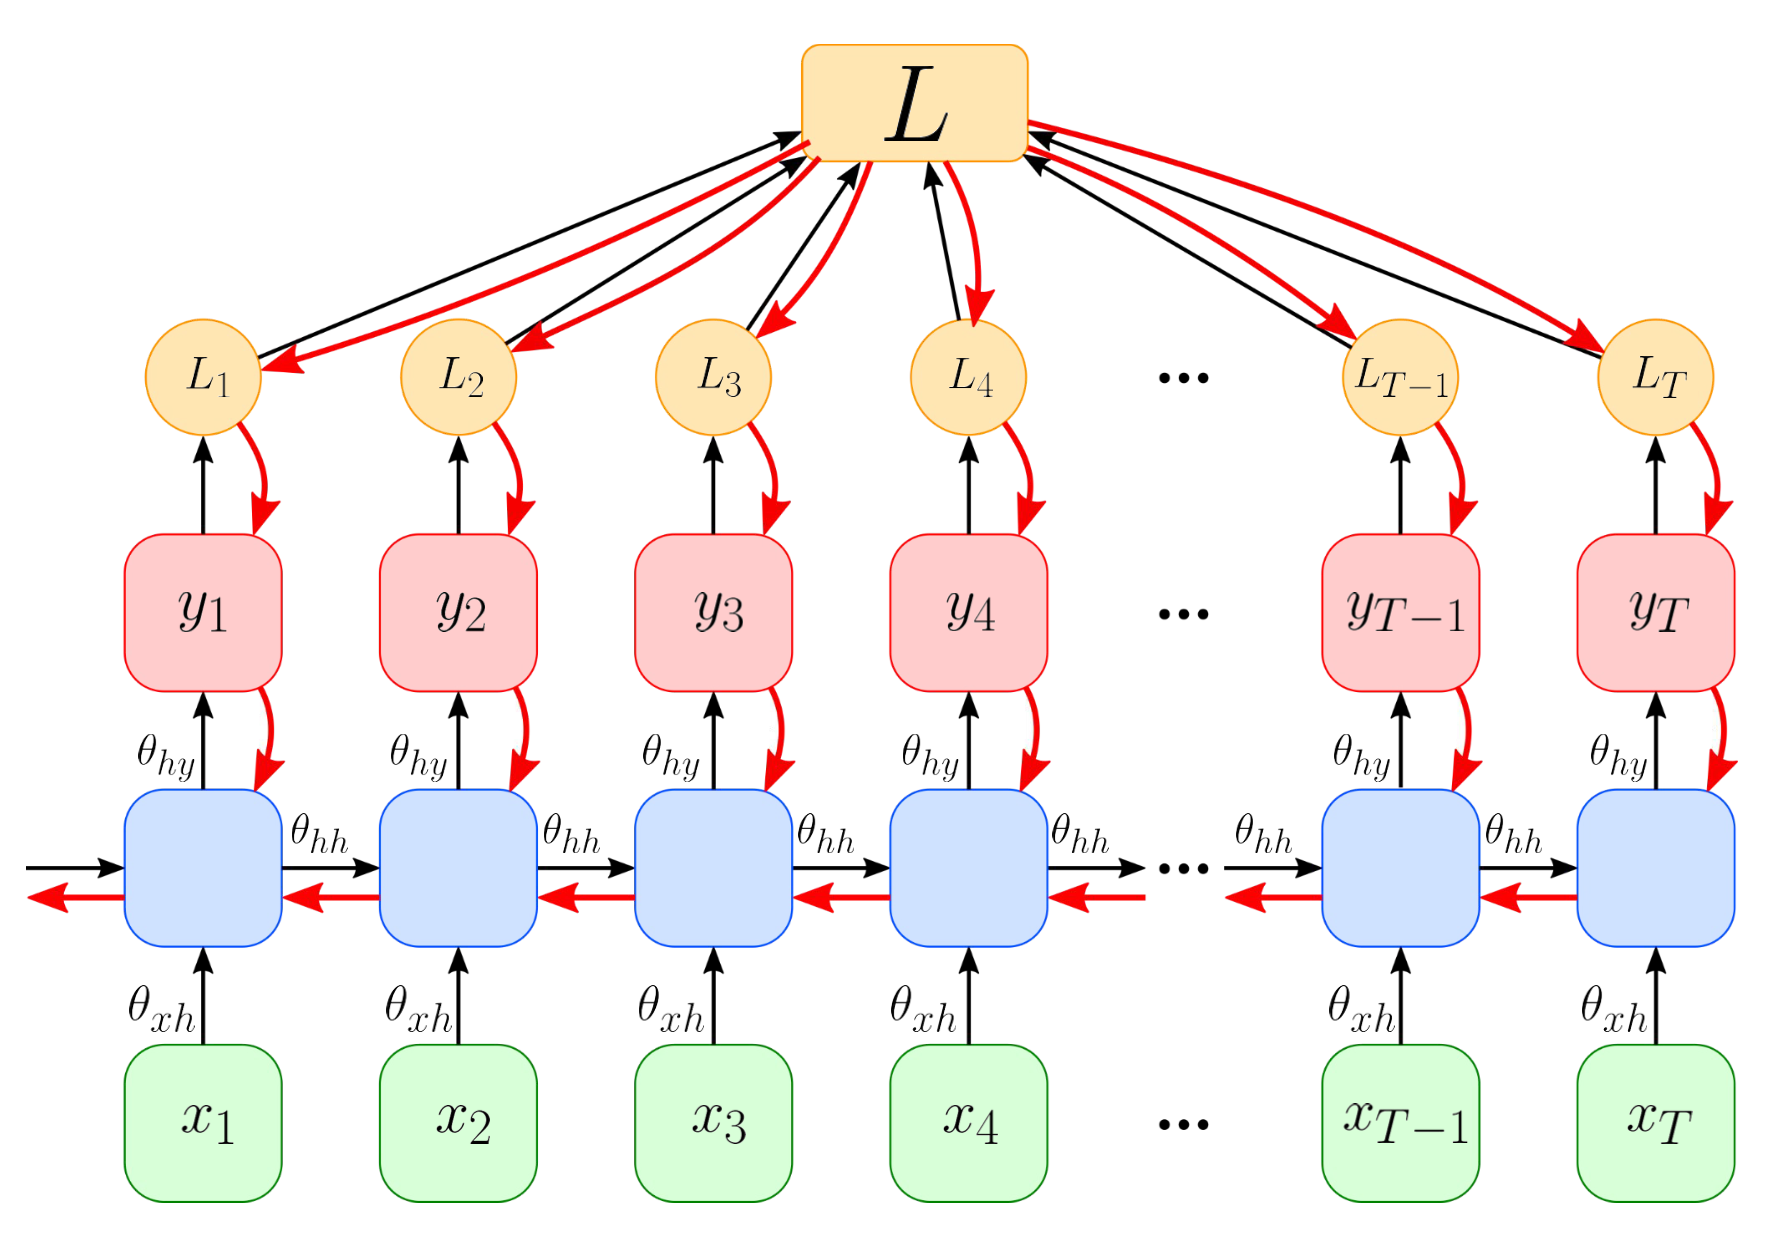
\includegraphics[width=\linewidth]{cs4248-rnn-bptt.png}
    \item Problems with BPTT: vanishing gradients and time complexity. \textit{NOT} memory complexity.
    \item Mitigation: windowing: only backpropagate through a fixed number of time steps. The window size depends on VRAM limits.
    \item 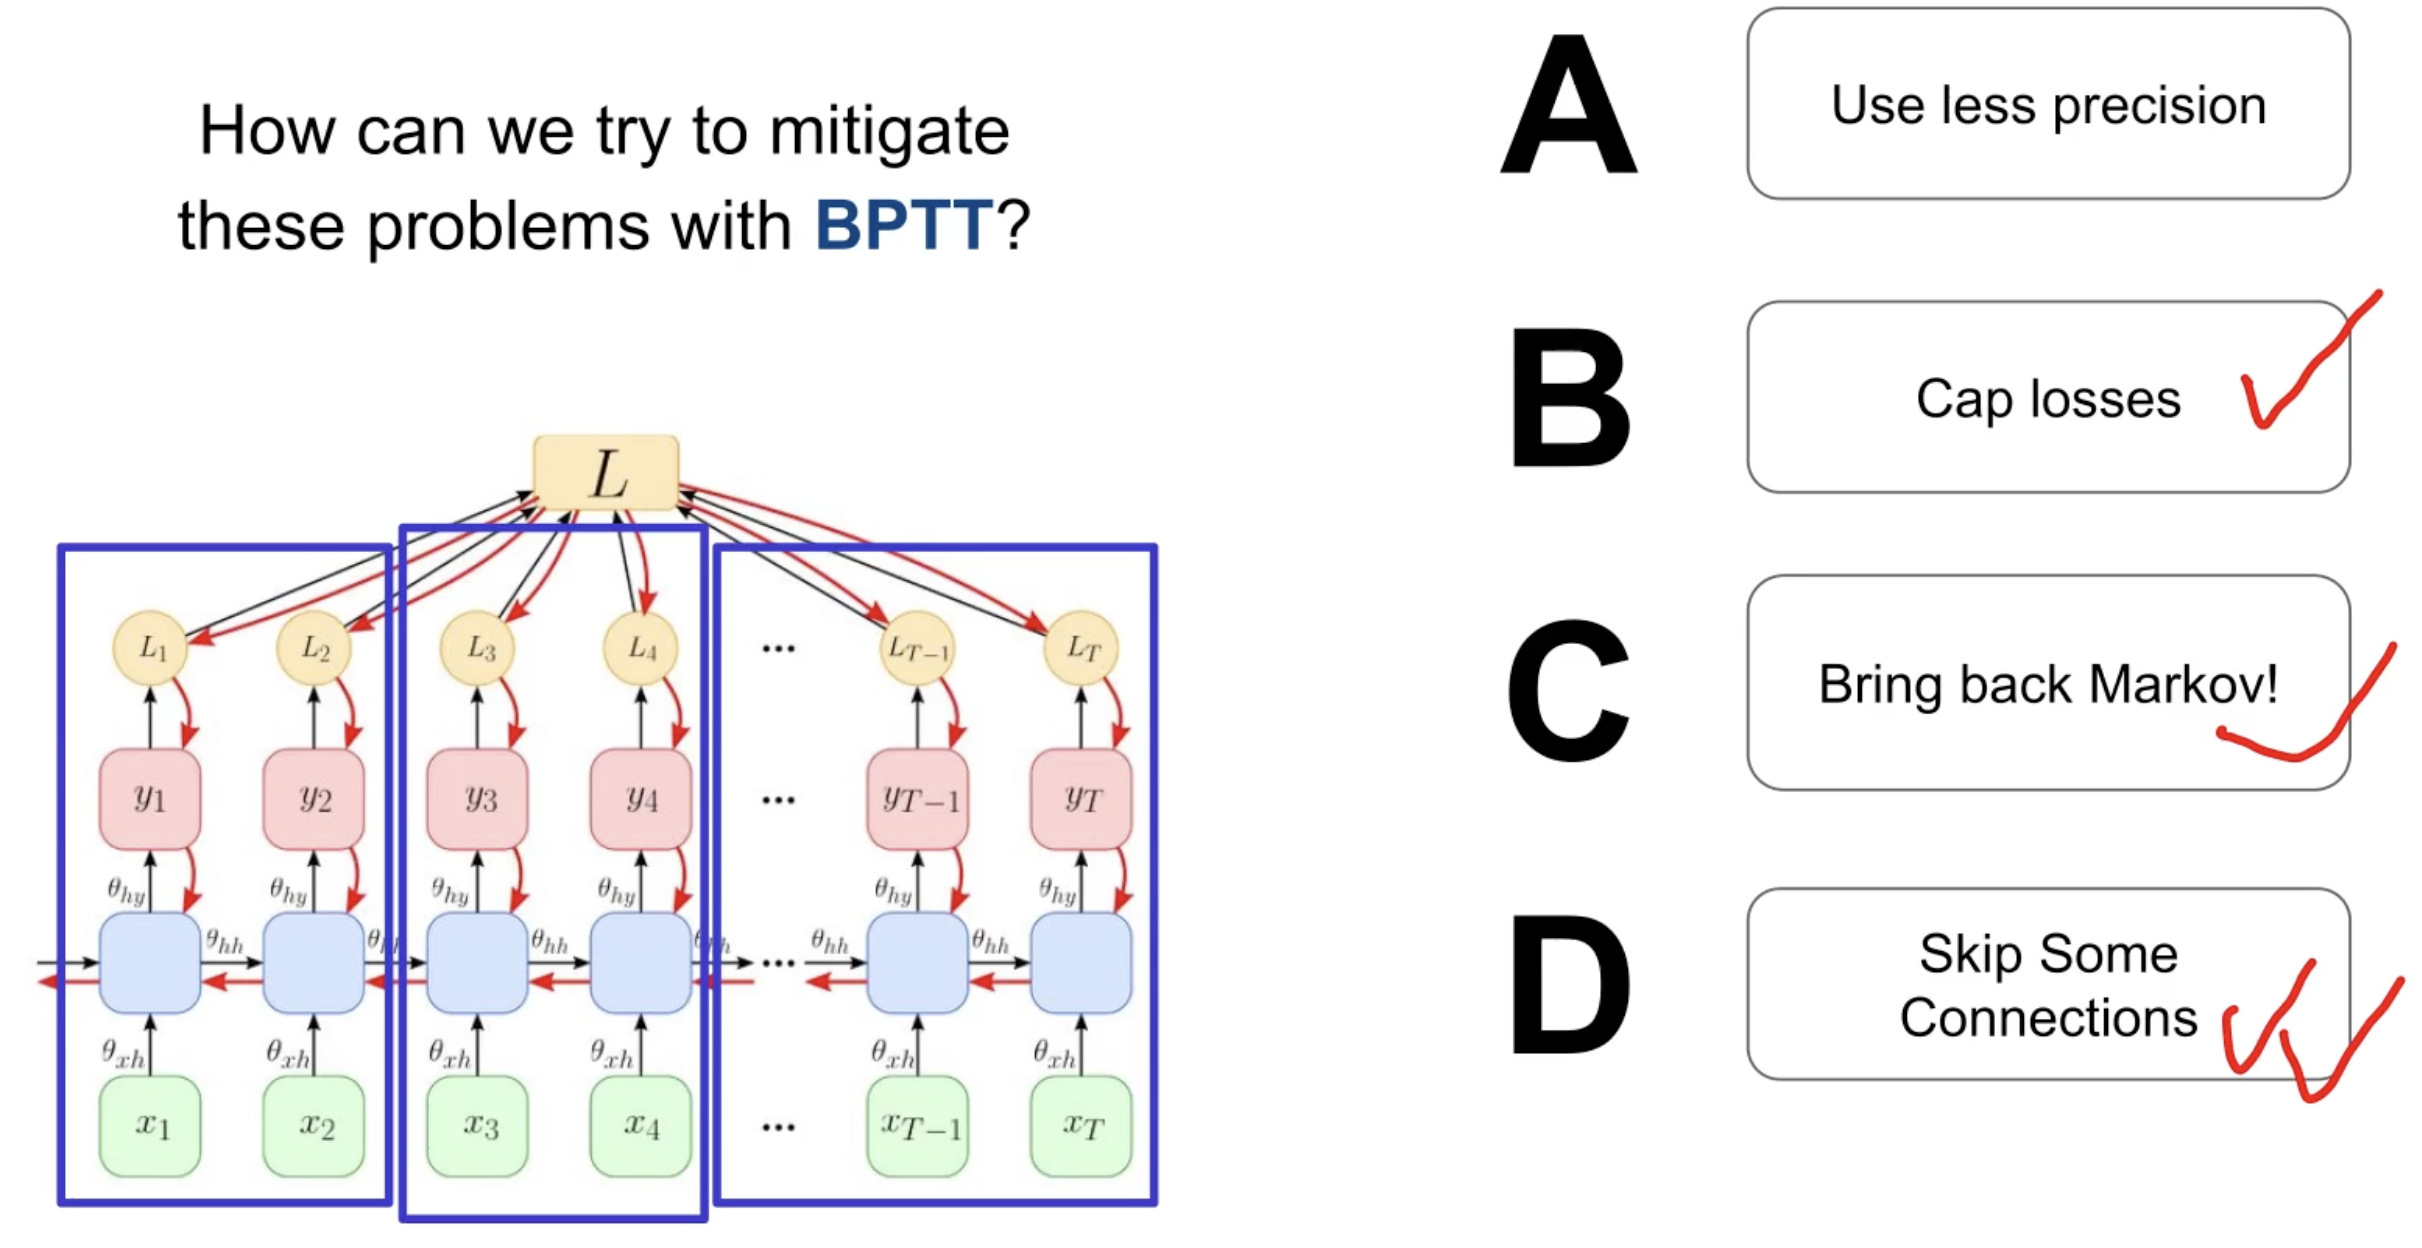
\includegraphics[width=0.8\linewidth]{cs4248-rnn-mitigate-bptt.png}
  \end{itemize}

  \subsection{Conditional RNNs}
  \subsubsection{Encoder-decoder}
  \begin{itemize}
    \item Encoder: Maps the \textbf{context} into a fixed-length vector $c$.
    \item Decoder: Maps the $c$ into a sequence of words.
    \item \textbf{Kalchbrenner and Blunsom (2013)}:
    \item \begin{itemize}
      \item $h_t = \sigma(\theta_{hh} h_{t-1} + \theta_{xh} x_t + \textcolor{red}{s})$, $y_t = \text{softmax}(\theta_{hy} h_t)$
    \end{itemize}
    \item \textbf{Sutskever et al. (2014)}:
    \item \begin{itemize}
      \item $h_t^{enc} = \sigma\left( \theta_{hh}^{enc} h_{t-1}^{enc} + \theta_{xh}^{enc} x_t \right)$, $y_t^{enc}$ is not computed.
      \item $h_t^{dec} = \sigma\left( \theta_{hh}^{dec} h_{t-1}^{dec} + \theta_{xh}^{dec} x_t \right)$, $y_t^{dec} = \text{softmax}(\theta_{hy}^{dec} h_t^{dec})$
      \item \textbf{IMPT}: $h_0^{dec} = h_T^{enc}$
      \item 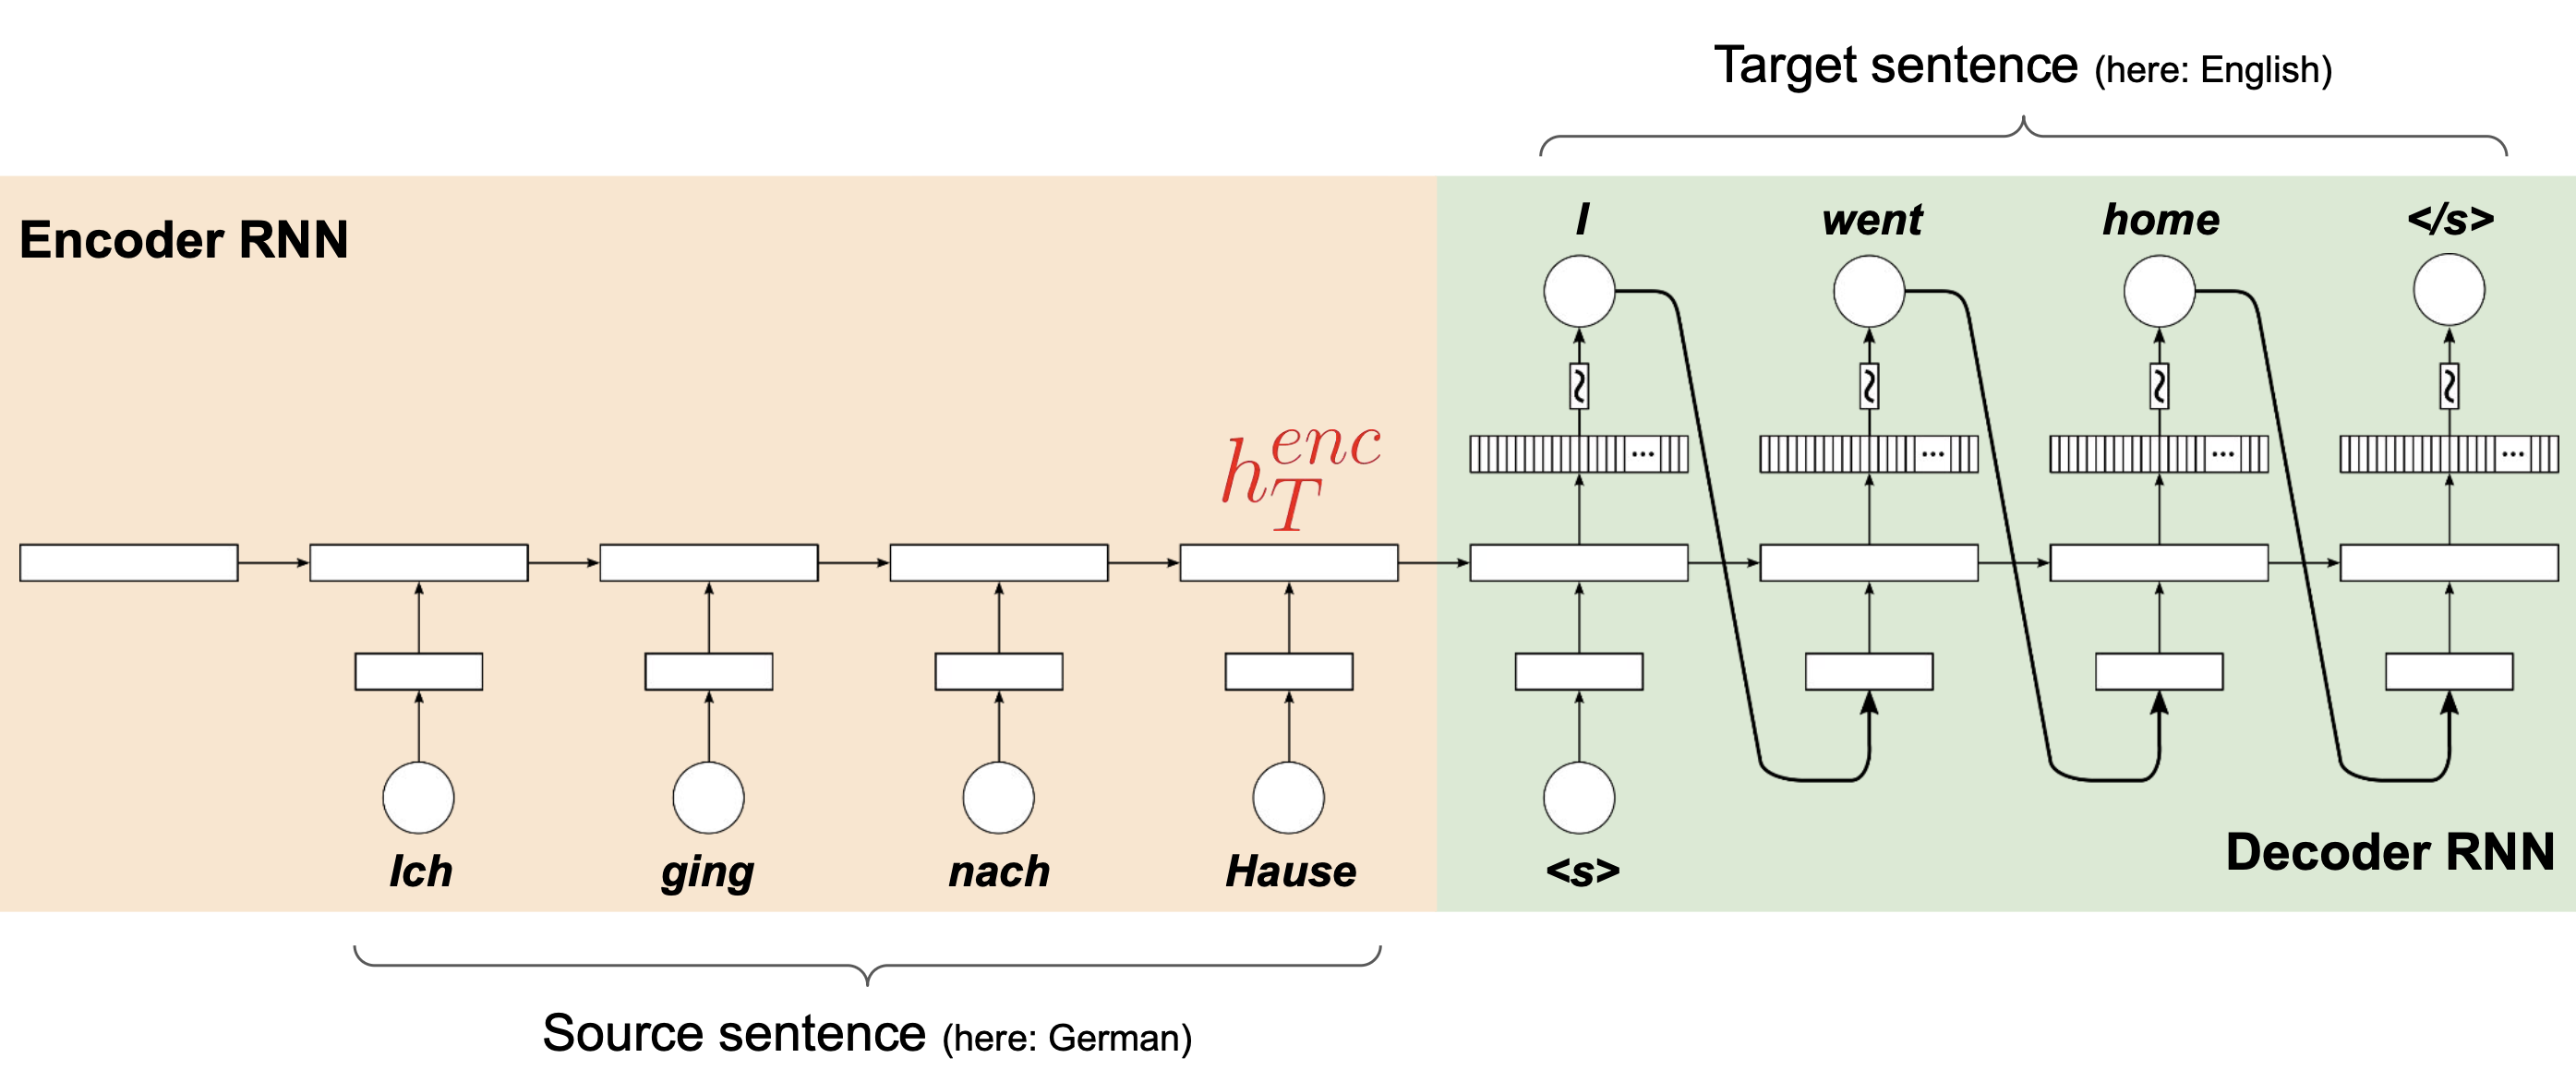
\includegraphics[width=0.9\linewidth]{cs4248-rnn-encdec.png}
    \end{itemize}
  \end{itemize}

  \subsection{Attention}
  \begin{itemize}
    \item \textbf{Motivation}: $c$ (e.g. $h_T^{enc}$) is used to represent the entire input sequence (\textit{bottleneck}).
    \item \begin{enumerate}
      \item Attention score (using dot product here): $e = [h_t^\top h_s^{(1)}, h_t^\top h_s^{(2)}, \ldots, h_t^\top h_s^{(N)}] \in \mathbb{R}^N$
      \item Attention weights: $\alpha = \text{softmax}(e) \in \mathbb{R}^N$
      \item Context vector: $c_t = \sum_{i=1}^N \alpha_i h_s^{(i)} \in \mathbb{R}^H$
      \item (vanilla) $y_t = \text{softmax}(\theta_{hy} [c_t, h_t])$
    \end{enumerate}
    \item "Query" $h_t$ is the decoder hidden state. "Key"/"Value" $h_s^{(i)}$ is the encoder hidden state.
  \end{itemize}

  \subsubsection{Beam search decoding}
  \begin{itemize}
    \item Motivation: Local optimal $\neq$ global optimal.
    \item Idea: Keep track of the top $k$ most likely sequences at each time step.
    \item \begin{itemize}
      \item Hypothesis: $Y_i = \{y_1, y_2, \ldots, y_t\}$
      \item score$(Y_i) = \log P(y_1, y_2, \ldots, y_t|x)$
    \end{itemize}
    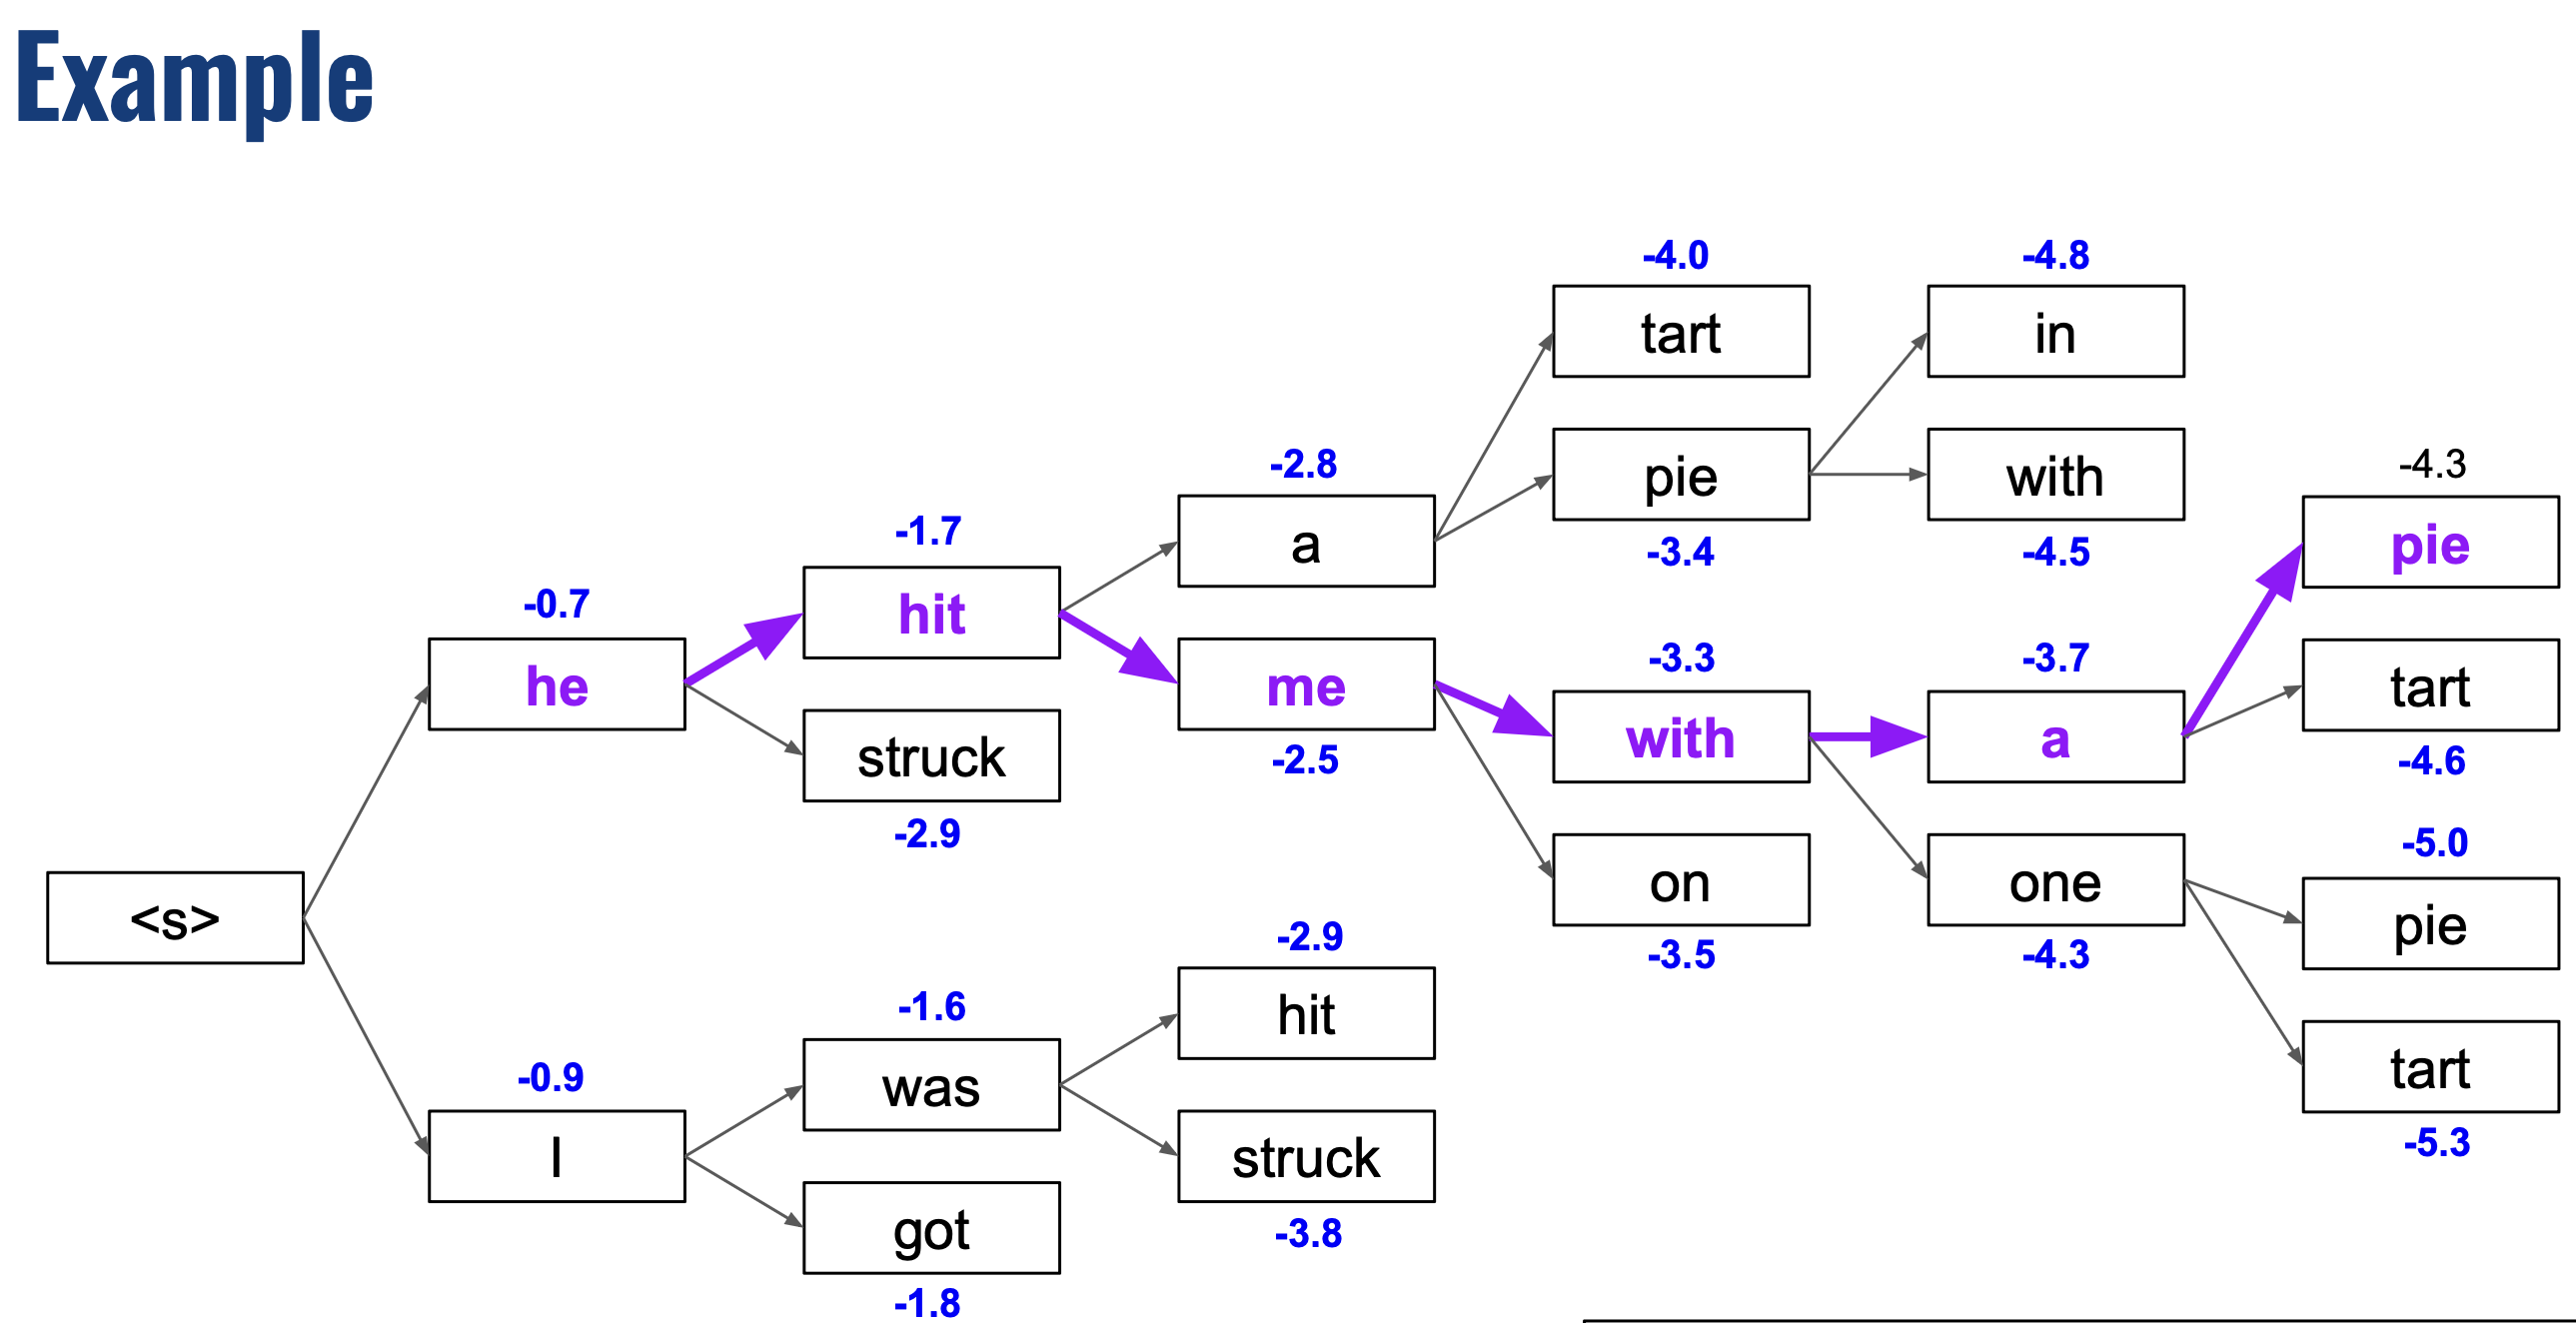
\includegraphics[width=\linewidth]{cs4248-rnn-beam-search.png}
    \item Different hypothesis produces \textless/s\textgreater\,at different steps.
    \item Stops when:
    \item \begin{itemize}
    \item A maximum of $T$ steps is reached,
    \item At least $n$ hypotheses have produced \textless/s\textgreater.
    \end{itemize}
    \item Sampling:
    \item \begin{itemize}
      \item Pure sampling: Sample $k$ words from the entire vocabulary based on the probability distribution.
      \item Top-$m$ sampling: Sample $k$ words from the subset of the vocabulary consisting of $m$ most probable words.
    \end{itemize}
  \end{itemize}

  \section{9 - Trees}
  \subsection{Syntactic parsing}
  \begin{itemize}
    \item Constituent: group of words that behaves as a single unit. Sentences can be described as a hierarchical structure of constituents.
    \item Constituent tests: 
    \item \begin{itemize}
      \item Topicalization: can be moved around
      \item Proform substitution: can be substituted with it/that/them/then/there, etc.
      \item Fragment answers: can answer a question while retaining the meaning of the original sentence.
    \end{itemize}
  \end{itemize}
  
  \subsubsection{Context-free grammars}
  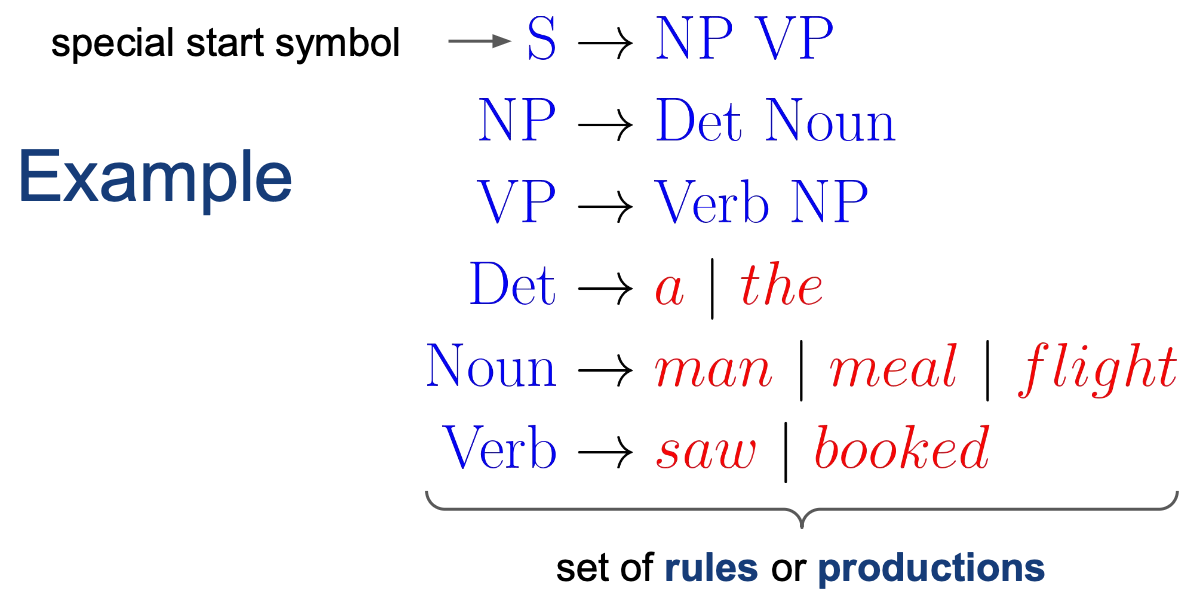
\includegraphics[width=\linewidth]{cs4248-trees-cfg.png}
  \begin{itemize}
    \item Definition: a 4-tuple ($N, \sum, R, S$)
    \item \begin{itemize}
      \item $N$ - set of non-terminal symbols
      \item $\sum$ - set of terminal symbols
      \item $R$ - set of rules
      \item $S$ - start symbol
    \end{itemize}
    \item \textbf{Requirements}: single non-terminal on LHS, application of rule does not depend on context.
  \end{itemize}
  \subsubsection{Structural ambiguity}
  \begin{itemize}
    \item Attachment ambiguity, coordination ambiguity.
  \end{itemize}
  \subsubsection{Chomsky Normal Form}
  \begin{itemize}
    \item Change in rules: only allow \textbf{1 terminal or 2 non-terminals} on RHS.
    \item Transform from CFG to CNF:
    \item \begin{itemize}
      \item Recursive removal of unary/empty rules: e.g. Nominal \textrightarrow\ Noun, Noun \textrightarrow\ book: Nominal \textrightarrow\ book, Noun \textrightarrow\ book.
      \item Dividing n-ary rules by introducing new non-terminals: e.g. S \textrightarrow\ Aux NP VP: S \textrightarrow\ X VP, X \textrightarrow\ Aux NP.
      \item Weak equivalence: generate the same set of sentences, but derivations may differ.
      \item Strong equivalence: identical expressiveness + identical derivations.
    \end{itemize}
  \end{itemize}

  \subsection{CYK Parsing}
  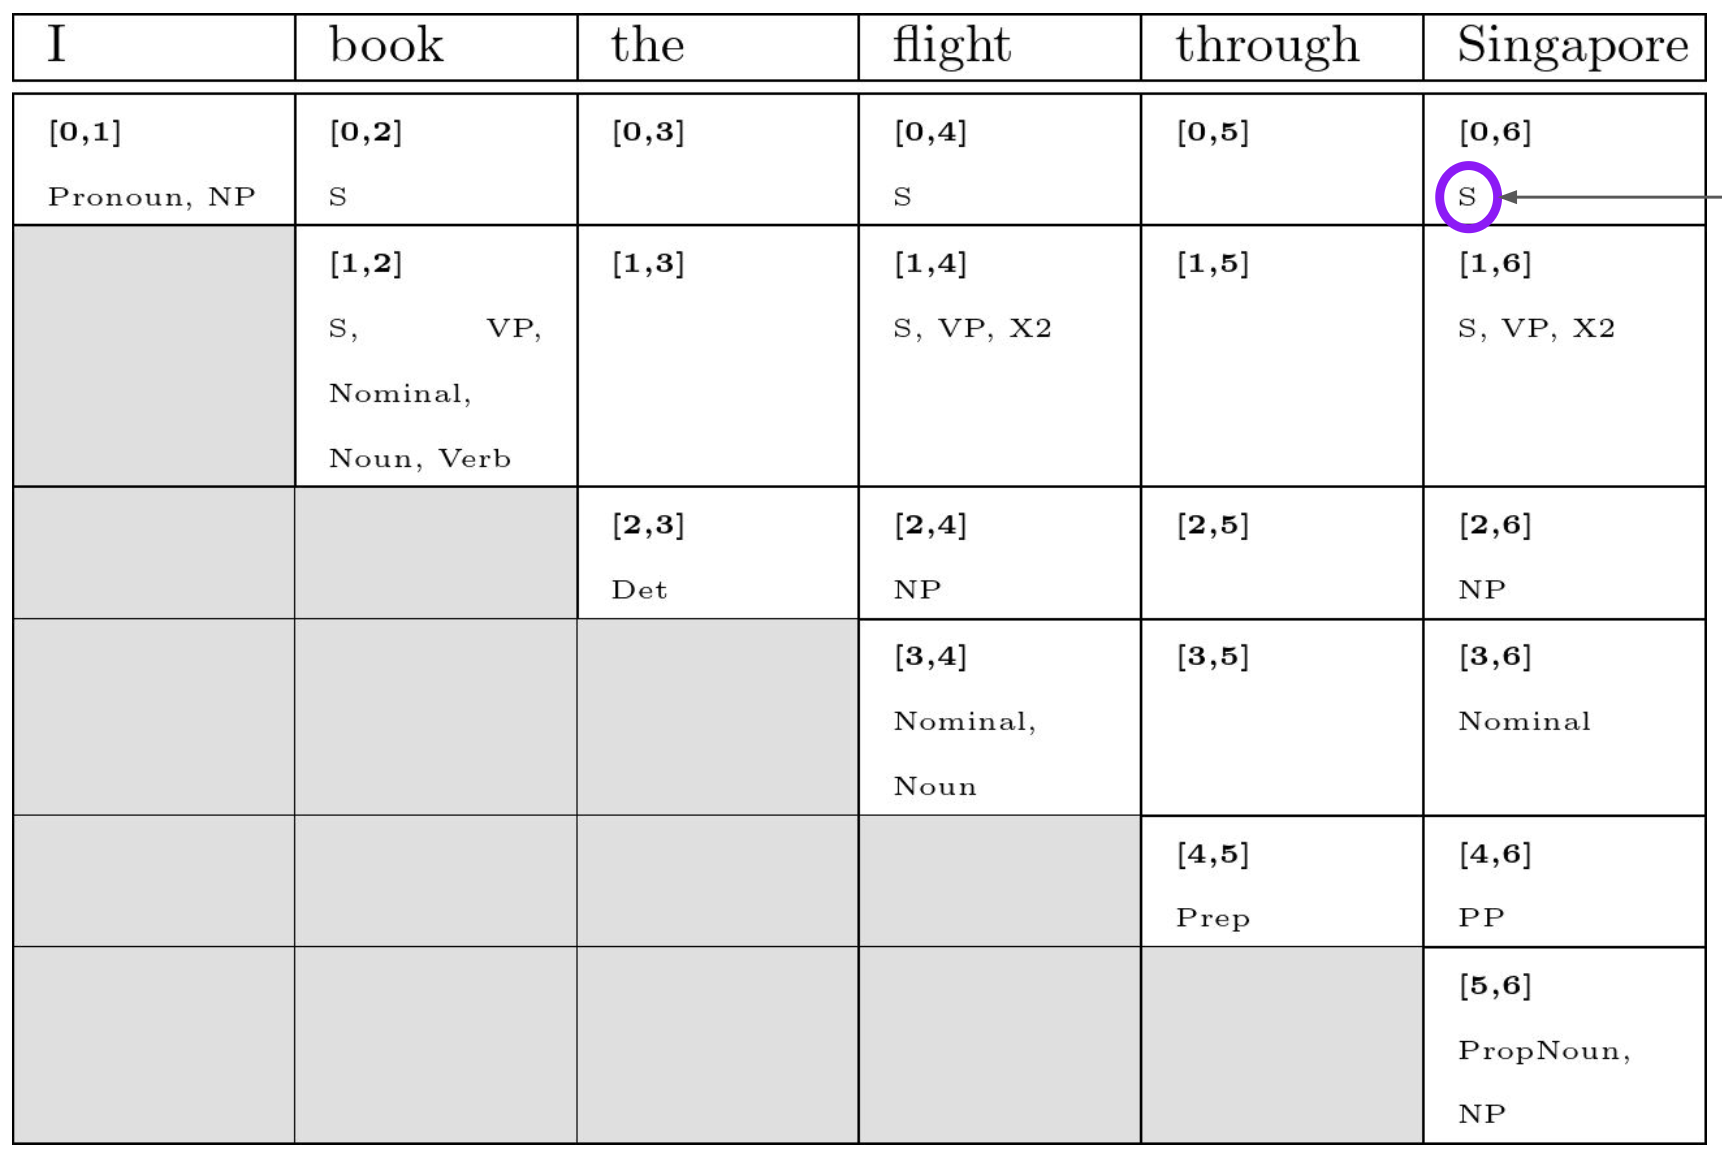
\includegraphics[width=\linewidth]{cs4248-trees-cyk.png}
  \begin{itemize}
    \item Valid sentence: "s" in the top right cell.
    \item Syntactic vs semantic (e.g. a "Noun" can be replaced by any noun)
  \end{itemize}
  An efficient form of a recursive top-down algorithm is the Earley parsing algorithm, which is still recursive but requires the algorithm to keep state; i.e., keep track of partially completed productions. This allows it to find a valid parse in some cases asymptotically faster than the O(n3) time required for CYK.
  \subsubsection{Get all parse trees}
  Very inaccurate pseudo code:
  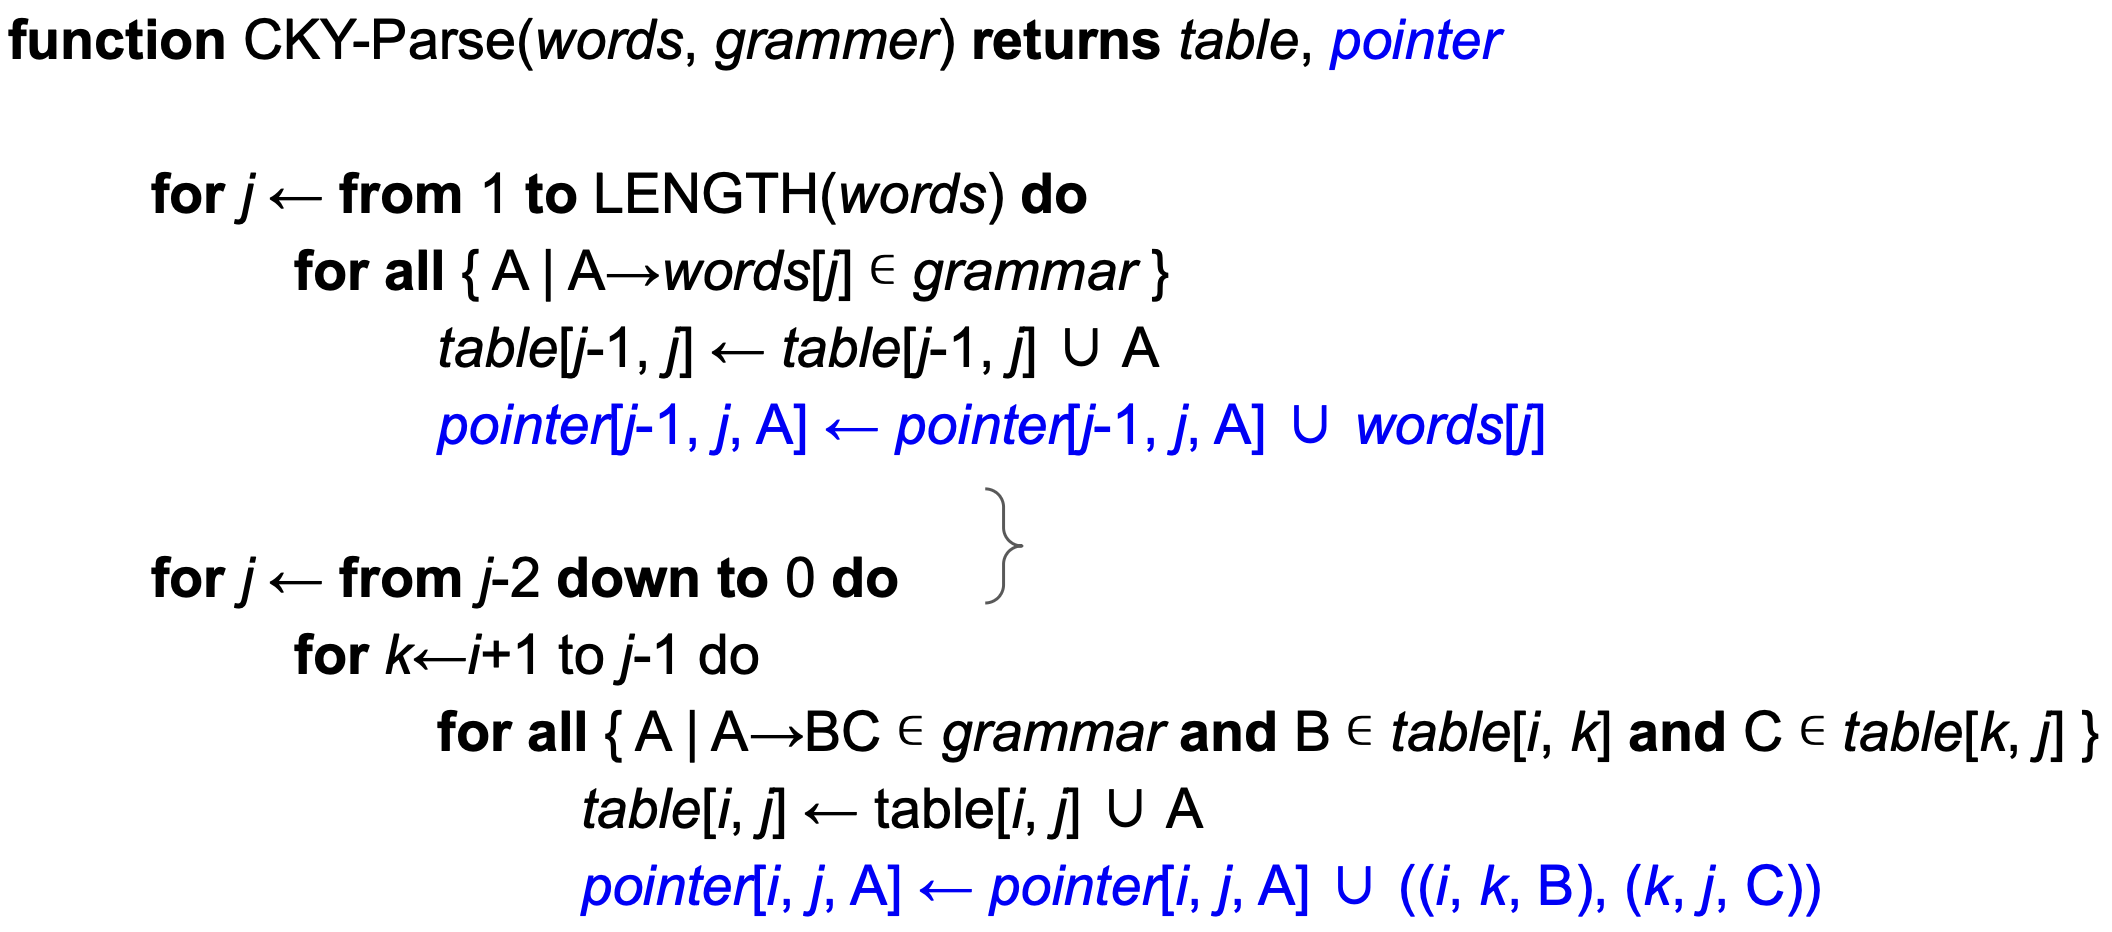
\includegraphics[width=\linewidth]{cs4248-trees-pseudocode.png}
  \subsubsection{Statistical parsing}
  \begin{itemize}
    \item Requirement for valid probabilities: $\sum_\alpha P(A\rightarrow\alpha) = 1$ (i.e. the sum of P for all rules with the same LHS is 1)
    \item Learning the probabilities: $P(A\rightarrow\alpha) = \frac{count(A\rightarrow\alpha)}{count(A)}$
    \item Converting PCFG to CNF:
    \item \begin{itemize}
      \item n-ary rules: S \textrightarrow\ Aux NP VP [0.1]: S \textrightarrow\ X1 VP [0.1], X1 \textrightarrow\ Aux NP [1.0]
      \item Removing unary rules:\\
      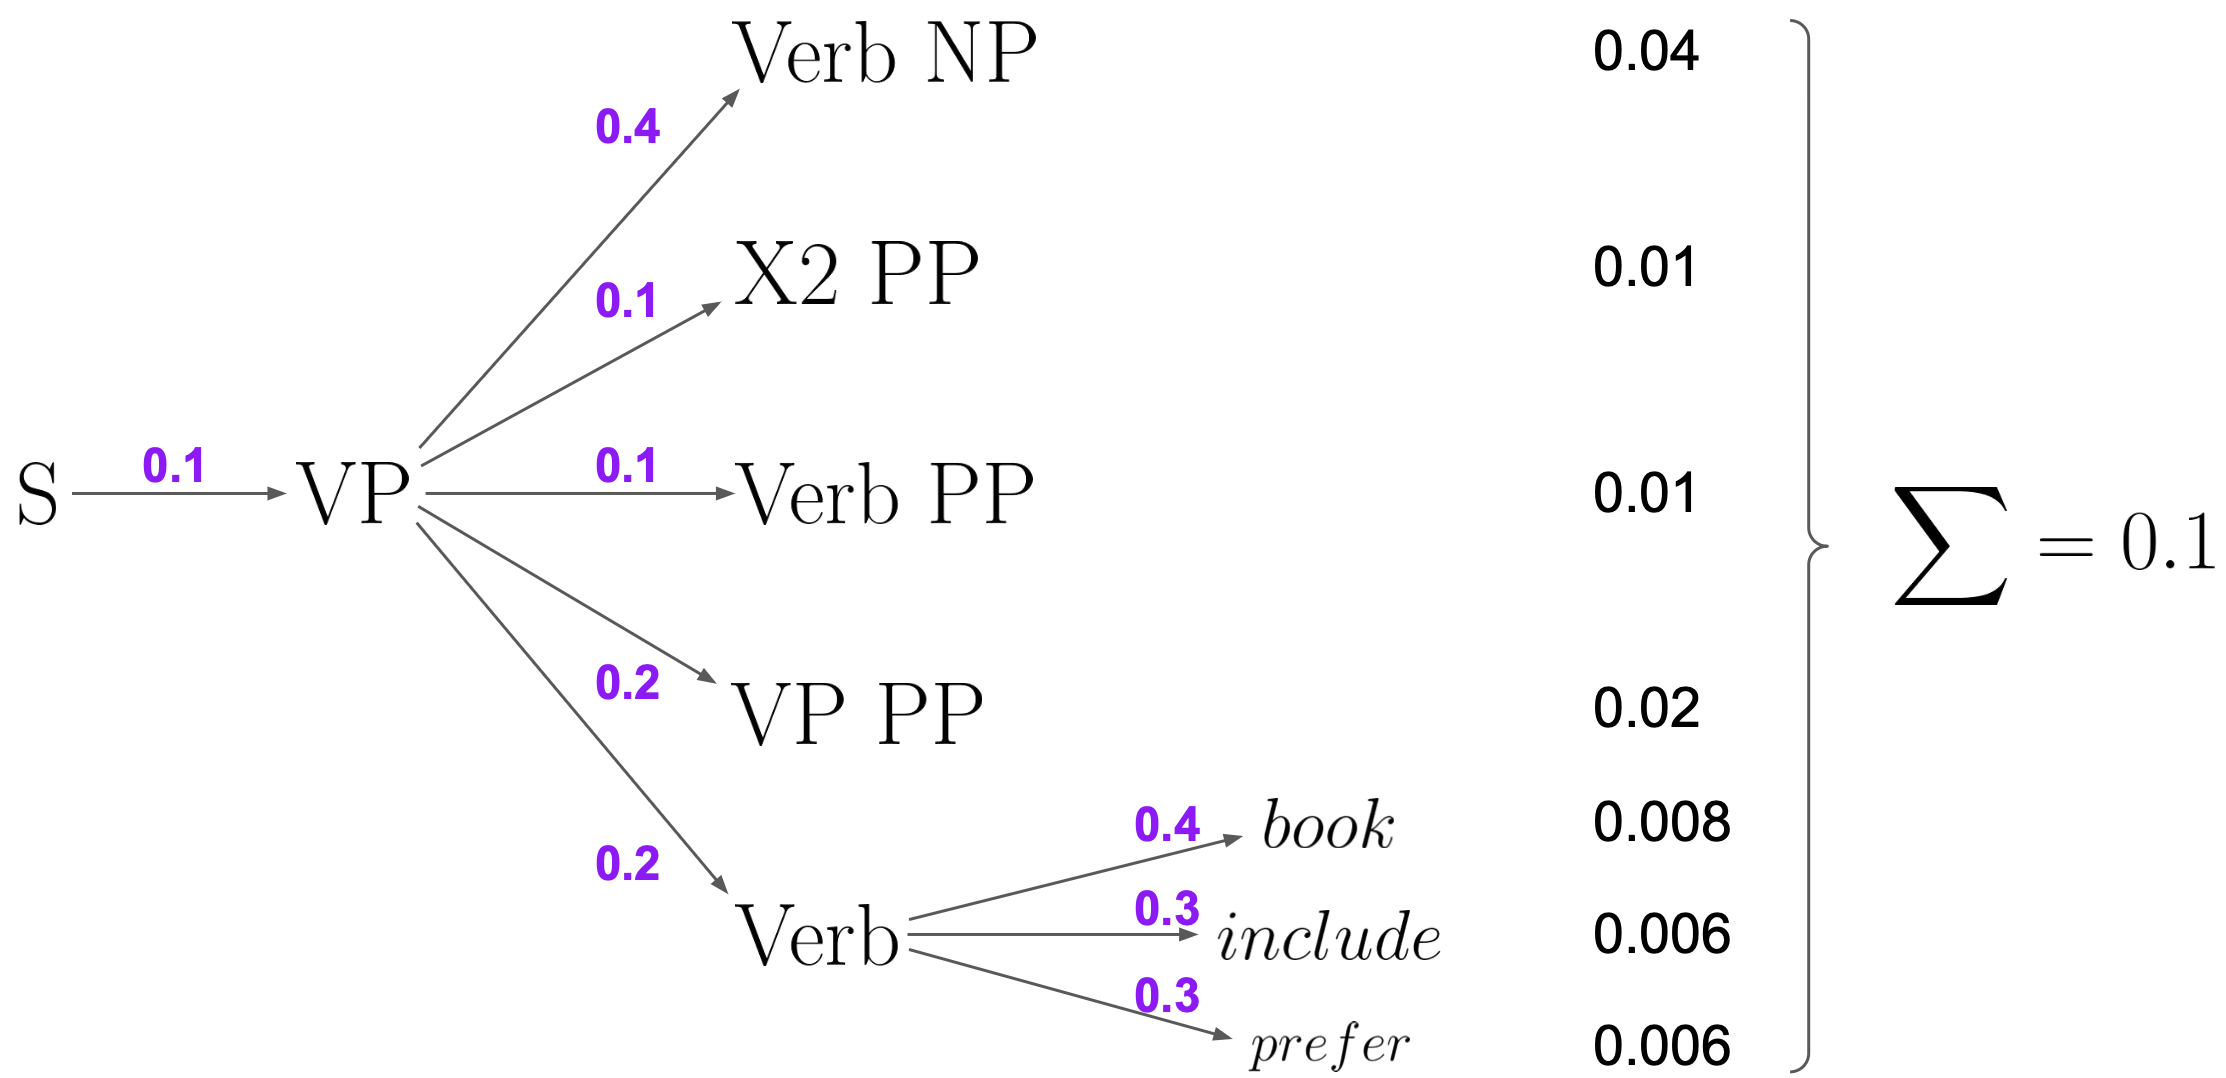
\includegraphics[width=\linewidth]{cs4248-trees-pcfgtocnf.png}
    \end{itemize}
  \end{itemize}
  \subsubsection{Evaluate parse trees}
  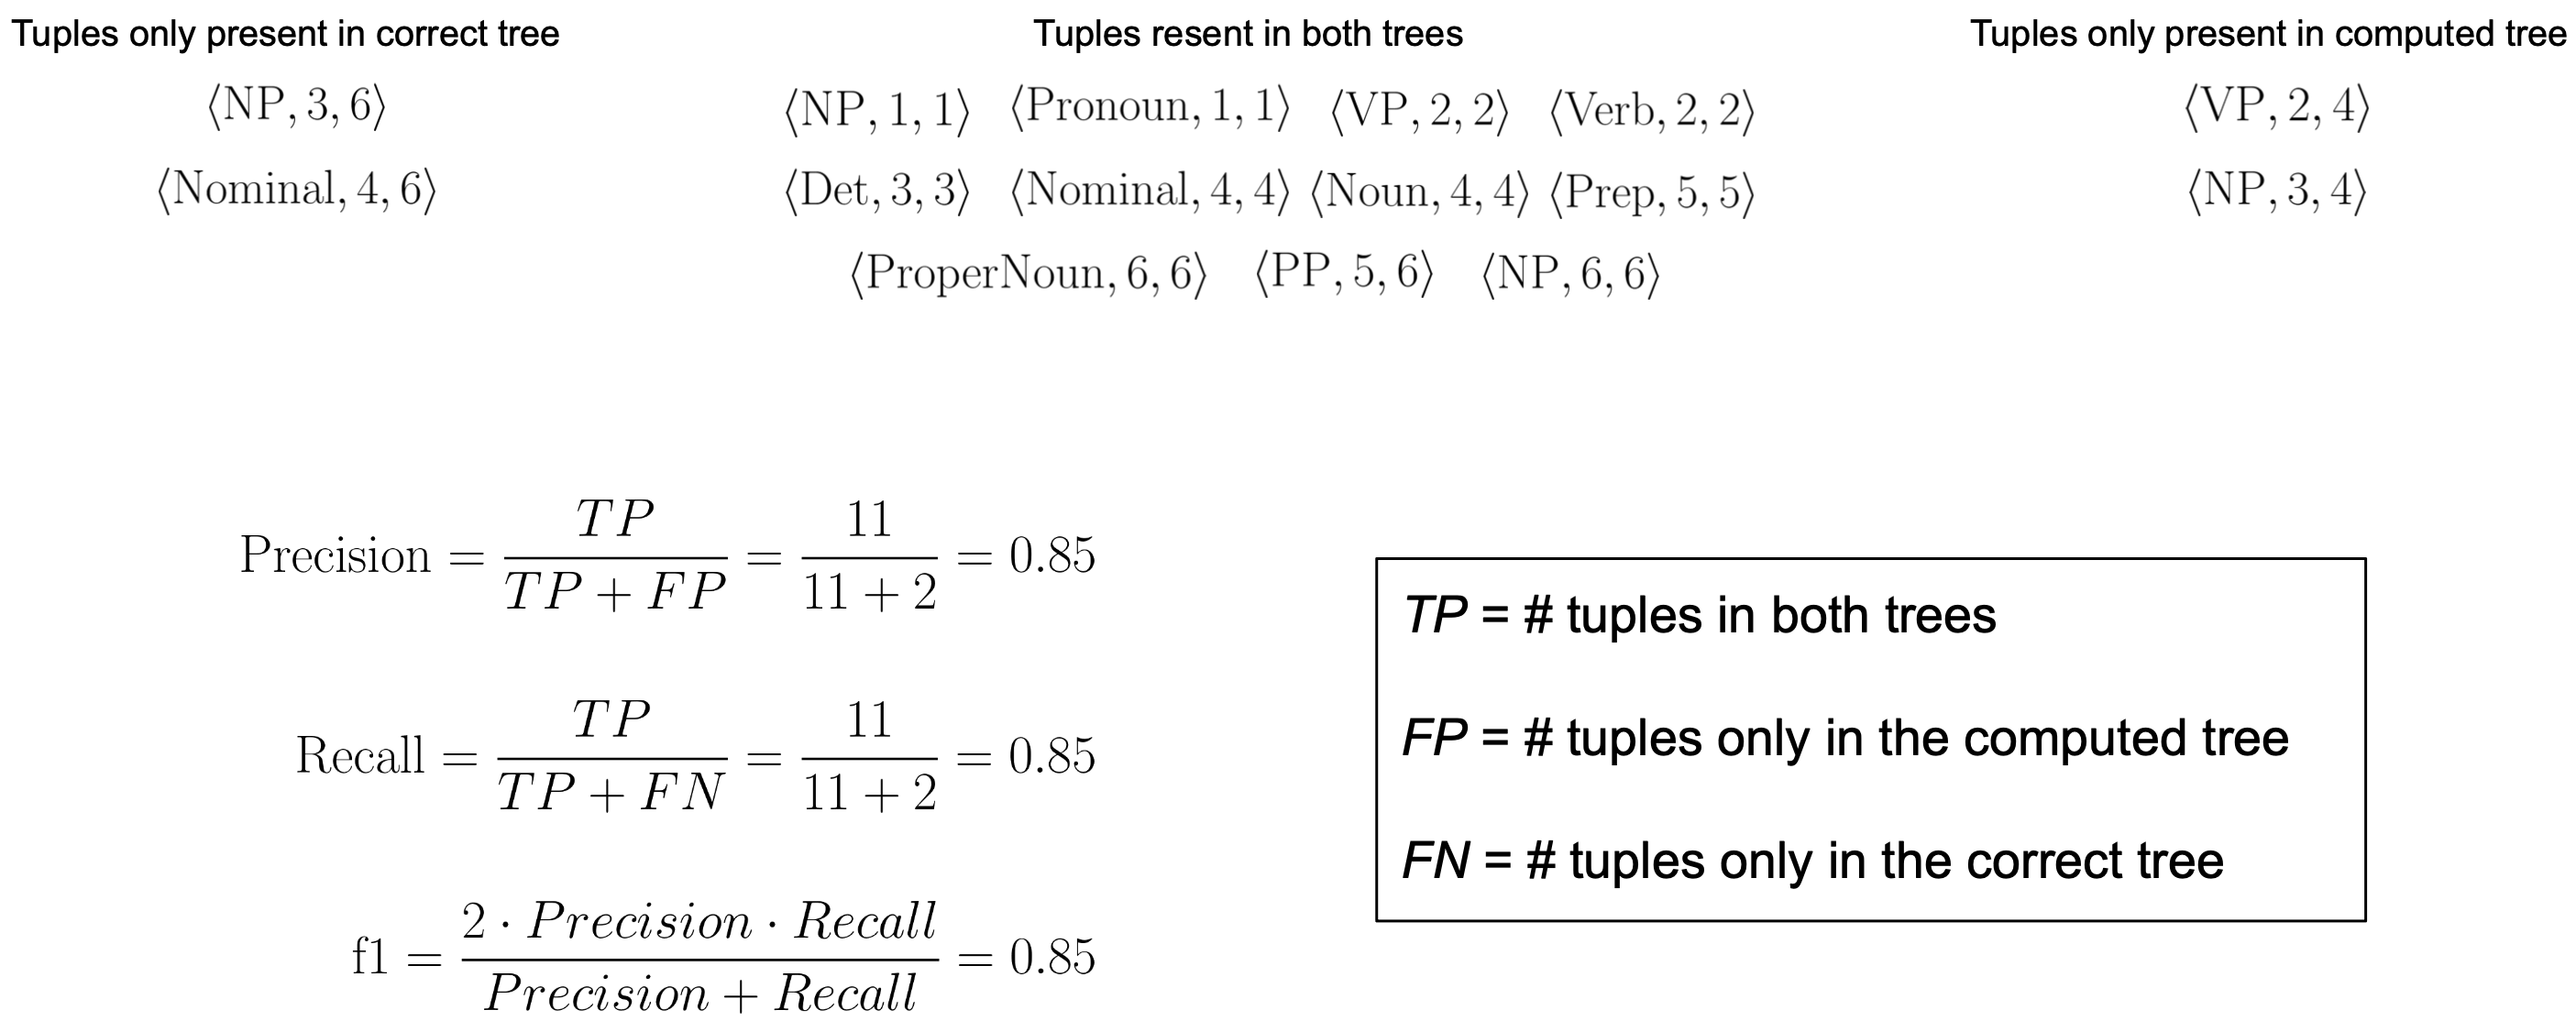
\includegraphics[width=\linewidth]{cs4248-trees-eval.png}
  \pagebreak

  \section{10 - Transformers}
  \begin{itemize}
    \item Motivation: Word representations should vary depending on the context. The context includes the whole sentence and the word order.
  \end{itemize}
  \subsubsection{ELMo}
  \begin{itemize}
    \item 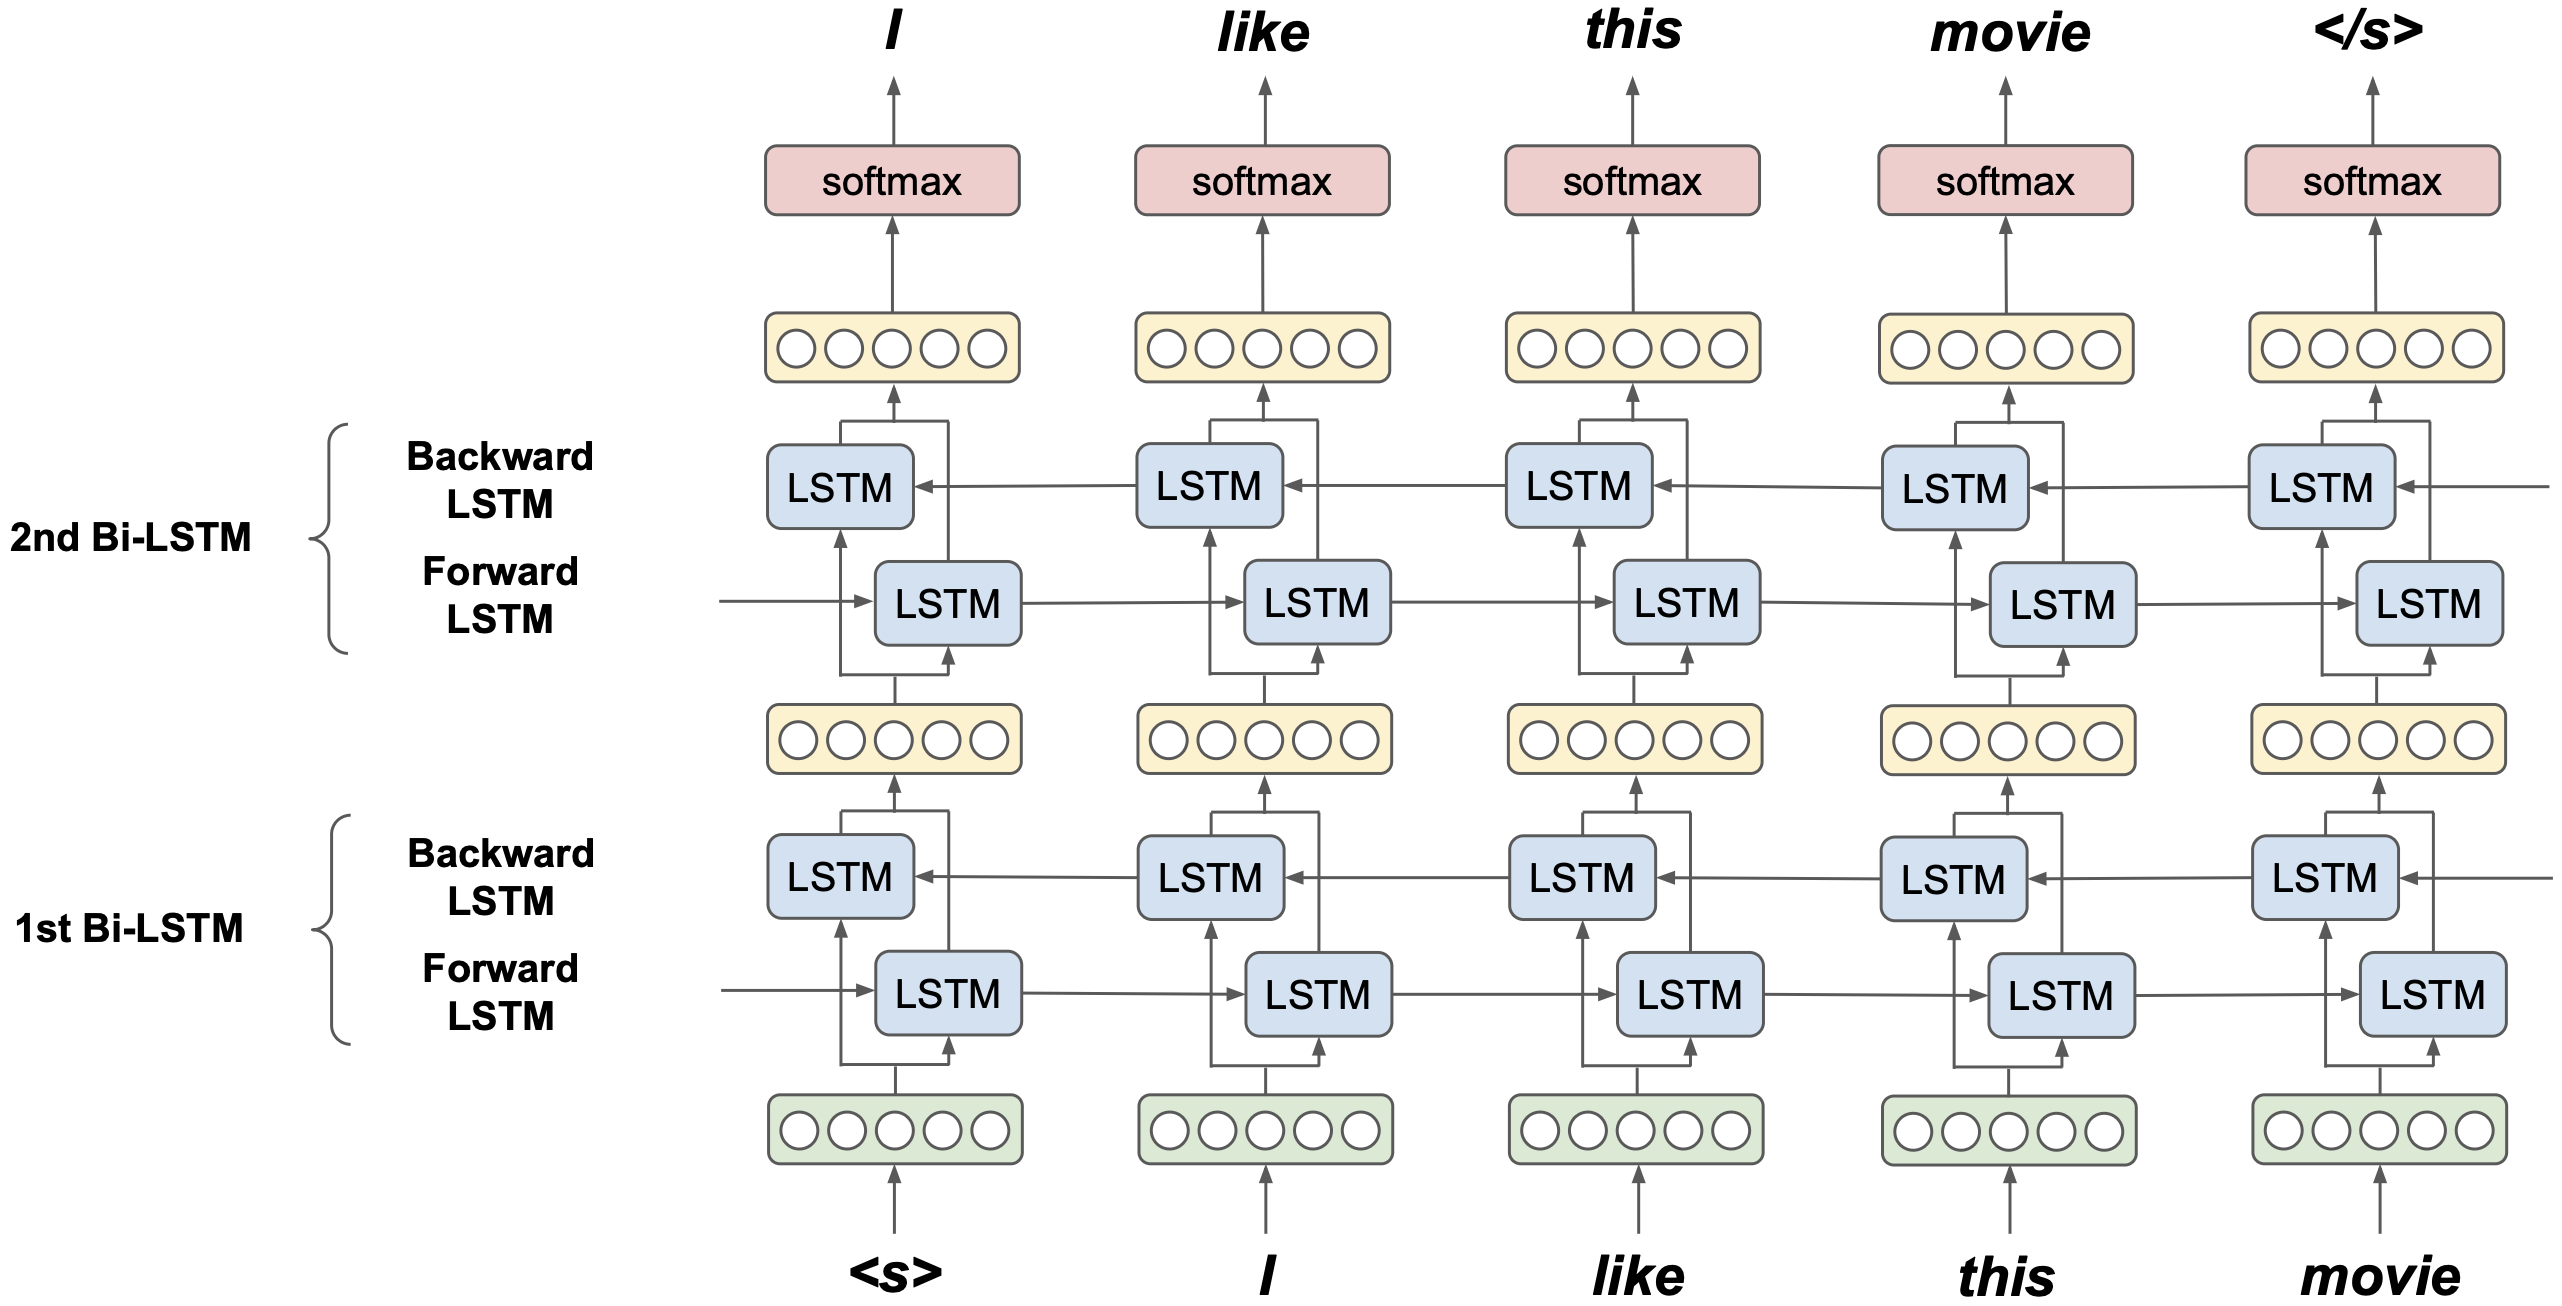
\includegraphics[width=0.7\linewidth]{cs4248-transformer-elmo.png}
    \item \textbf{Two layers of bi-LSTM}: After the first layer contextualize the embeddings, the second layer \textbf{re-contextualize} the embeddings. (e.g. "traffic" in "traffic light" learns its embeddings after the first layer, and "light" learns its embeddings based on the contextualized embeddings of "traffic" in the second layer.)
    \item \textbf{The final embedding} is usually a weighted sum of the two layers.
  \end{itemize}

  \subsection{Transformers}
  \begin{itemize}
    \item Encoder-decoder architecture without recurrence.
  \end{itemize}
  \subsection{Positional Encoding}
  \begin{itemize}
    \item \textbf{RNNs} process words sequentially, but \textbf{transformers} has no built-in notion of word order.
    \item Naive approaches include using the actual position (which quickly dominates the word embedding) or using $\frac{pos}{N-1}$ (encoding of the same position differs for different sentence lengths).
    \item Accepted approach: $\text{PE}_{(pos, 2i)} = \sin\left( \frac{pos}{10000^{2i/d_{model}}} \right)$, $\text{PE}_{(pos, 2i+1)} = \cos\left( \frac{pos}{10000^{2i/d_{model}}} \right)$
    \item 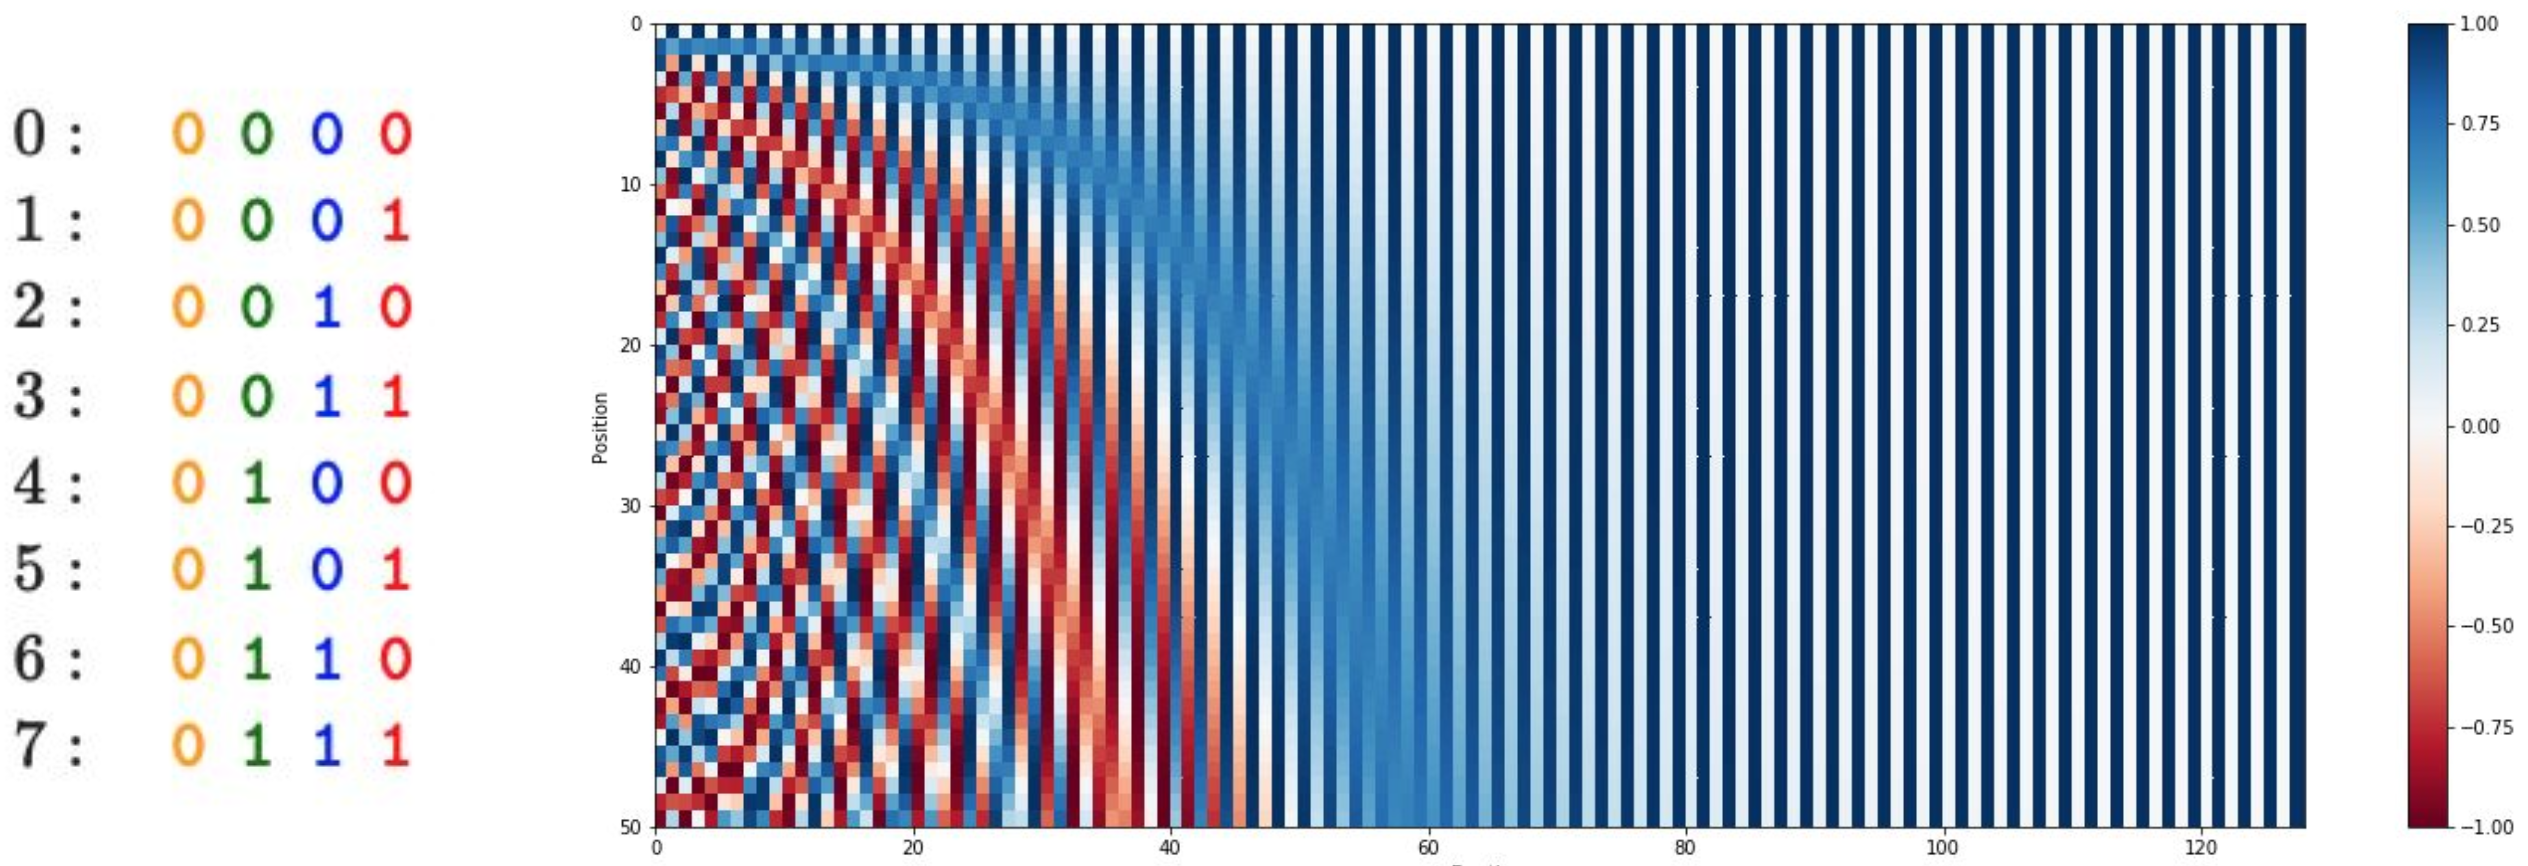
\includegraphics[width=\linewidth]{cs4248-transformer-pos-enc.png}
  \end{itemize}
  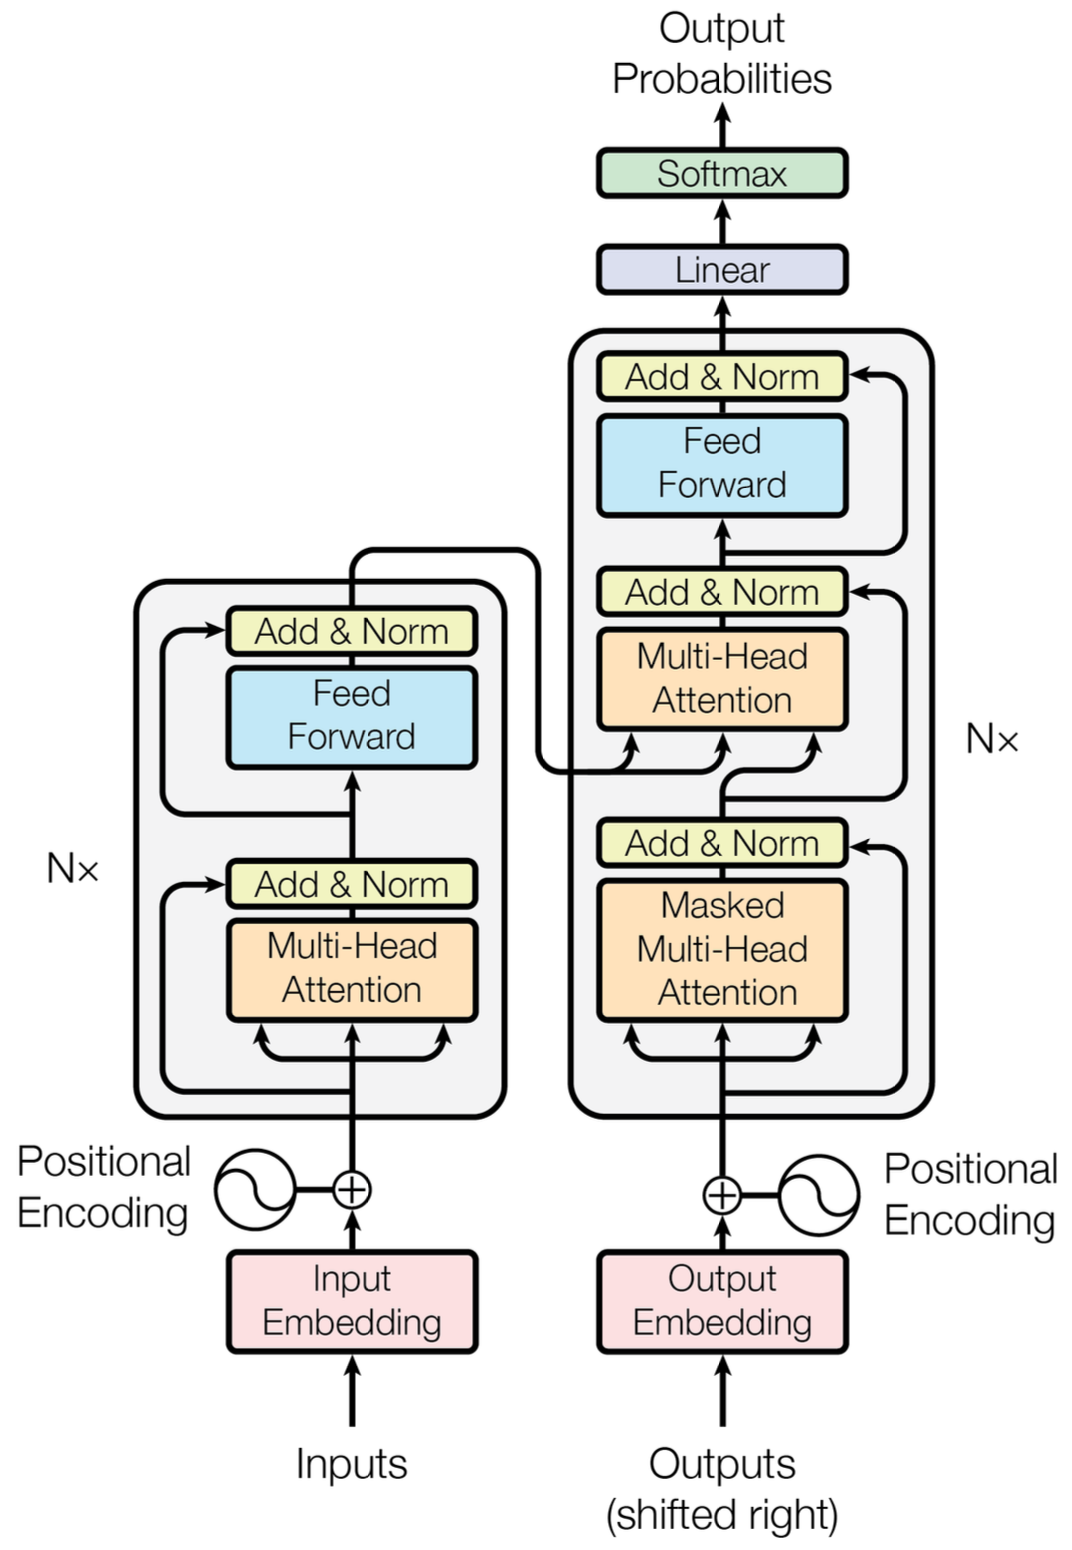
\includegraphics[width=\linewidth]{cs4248-transformer-architecture.png}
  \subsection{Encoder}
  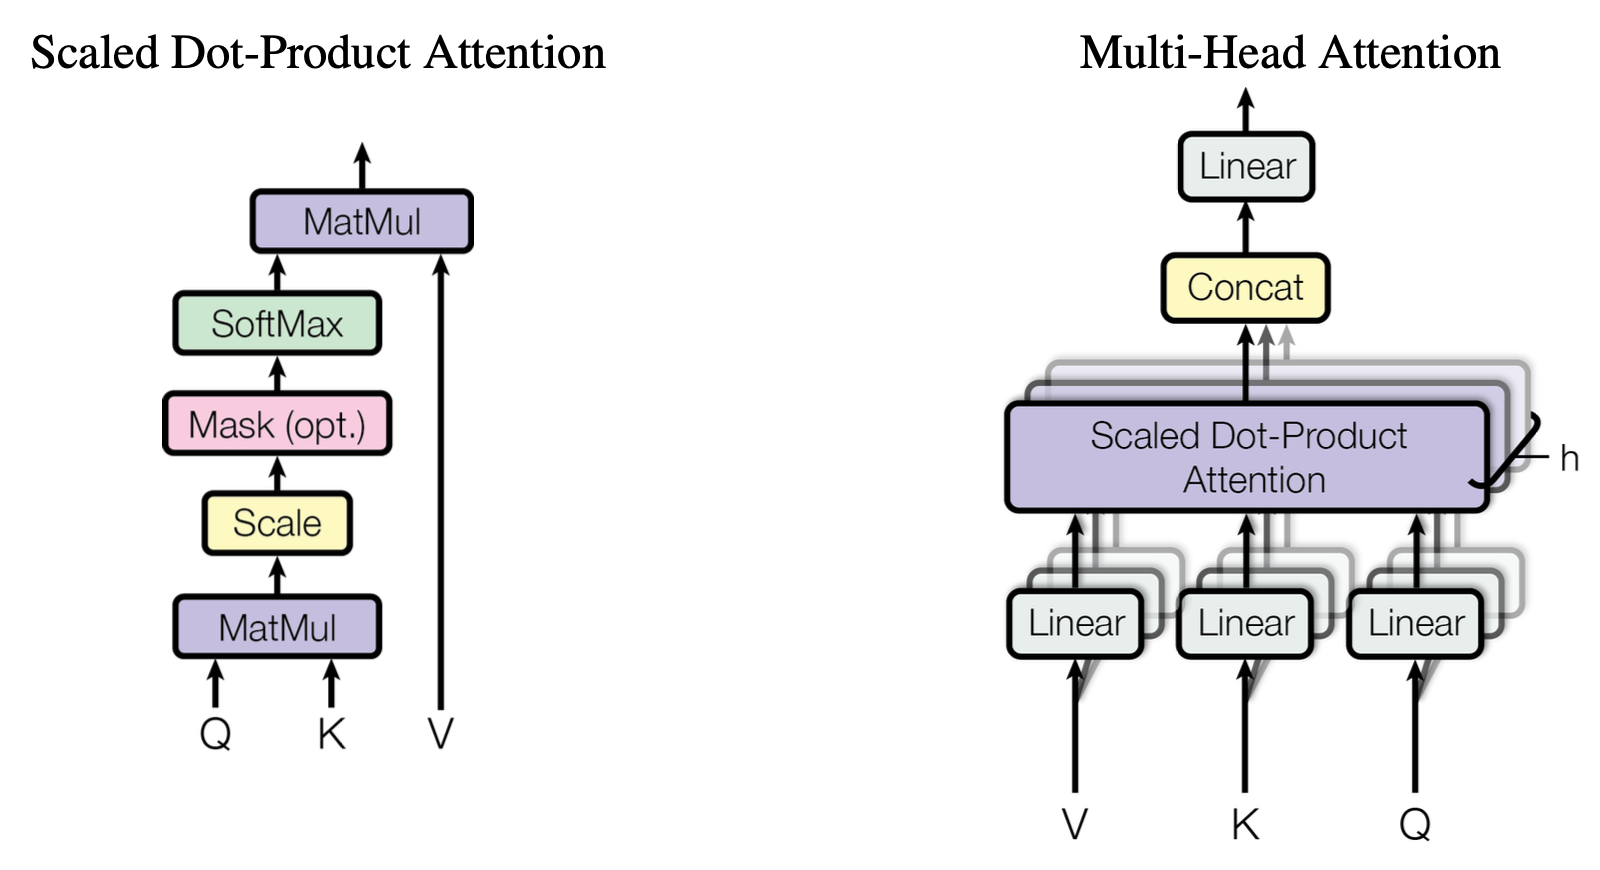
\includegraphics[width=\linewidth]{cs4248-transformer-mha.png}
  \begin{itemize}
    \item \textbf{Attention}: $\text{Attention}(Q,K,V) = \text{softmax}\left(\frac{QK^\top}{\sqrt{d_k}}\right)V$,
    \item 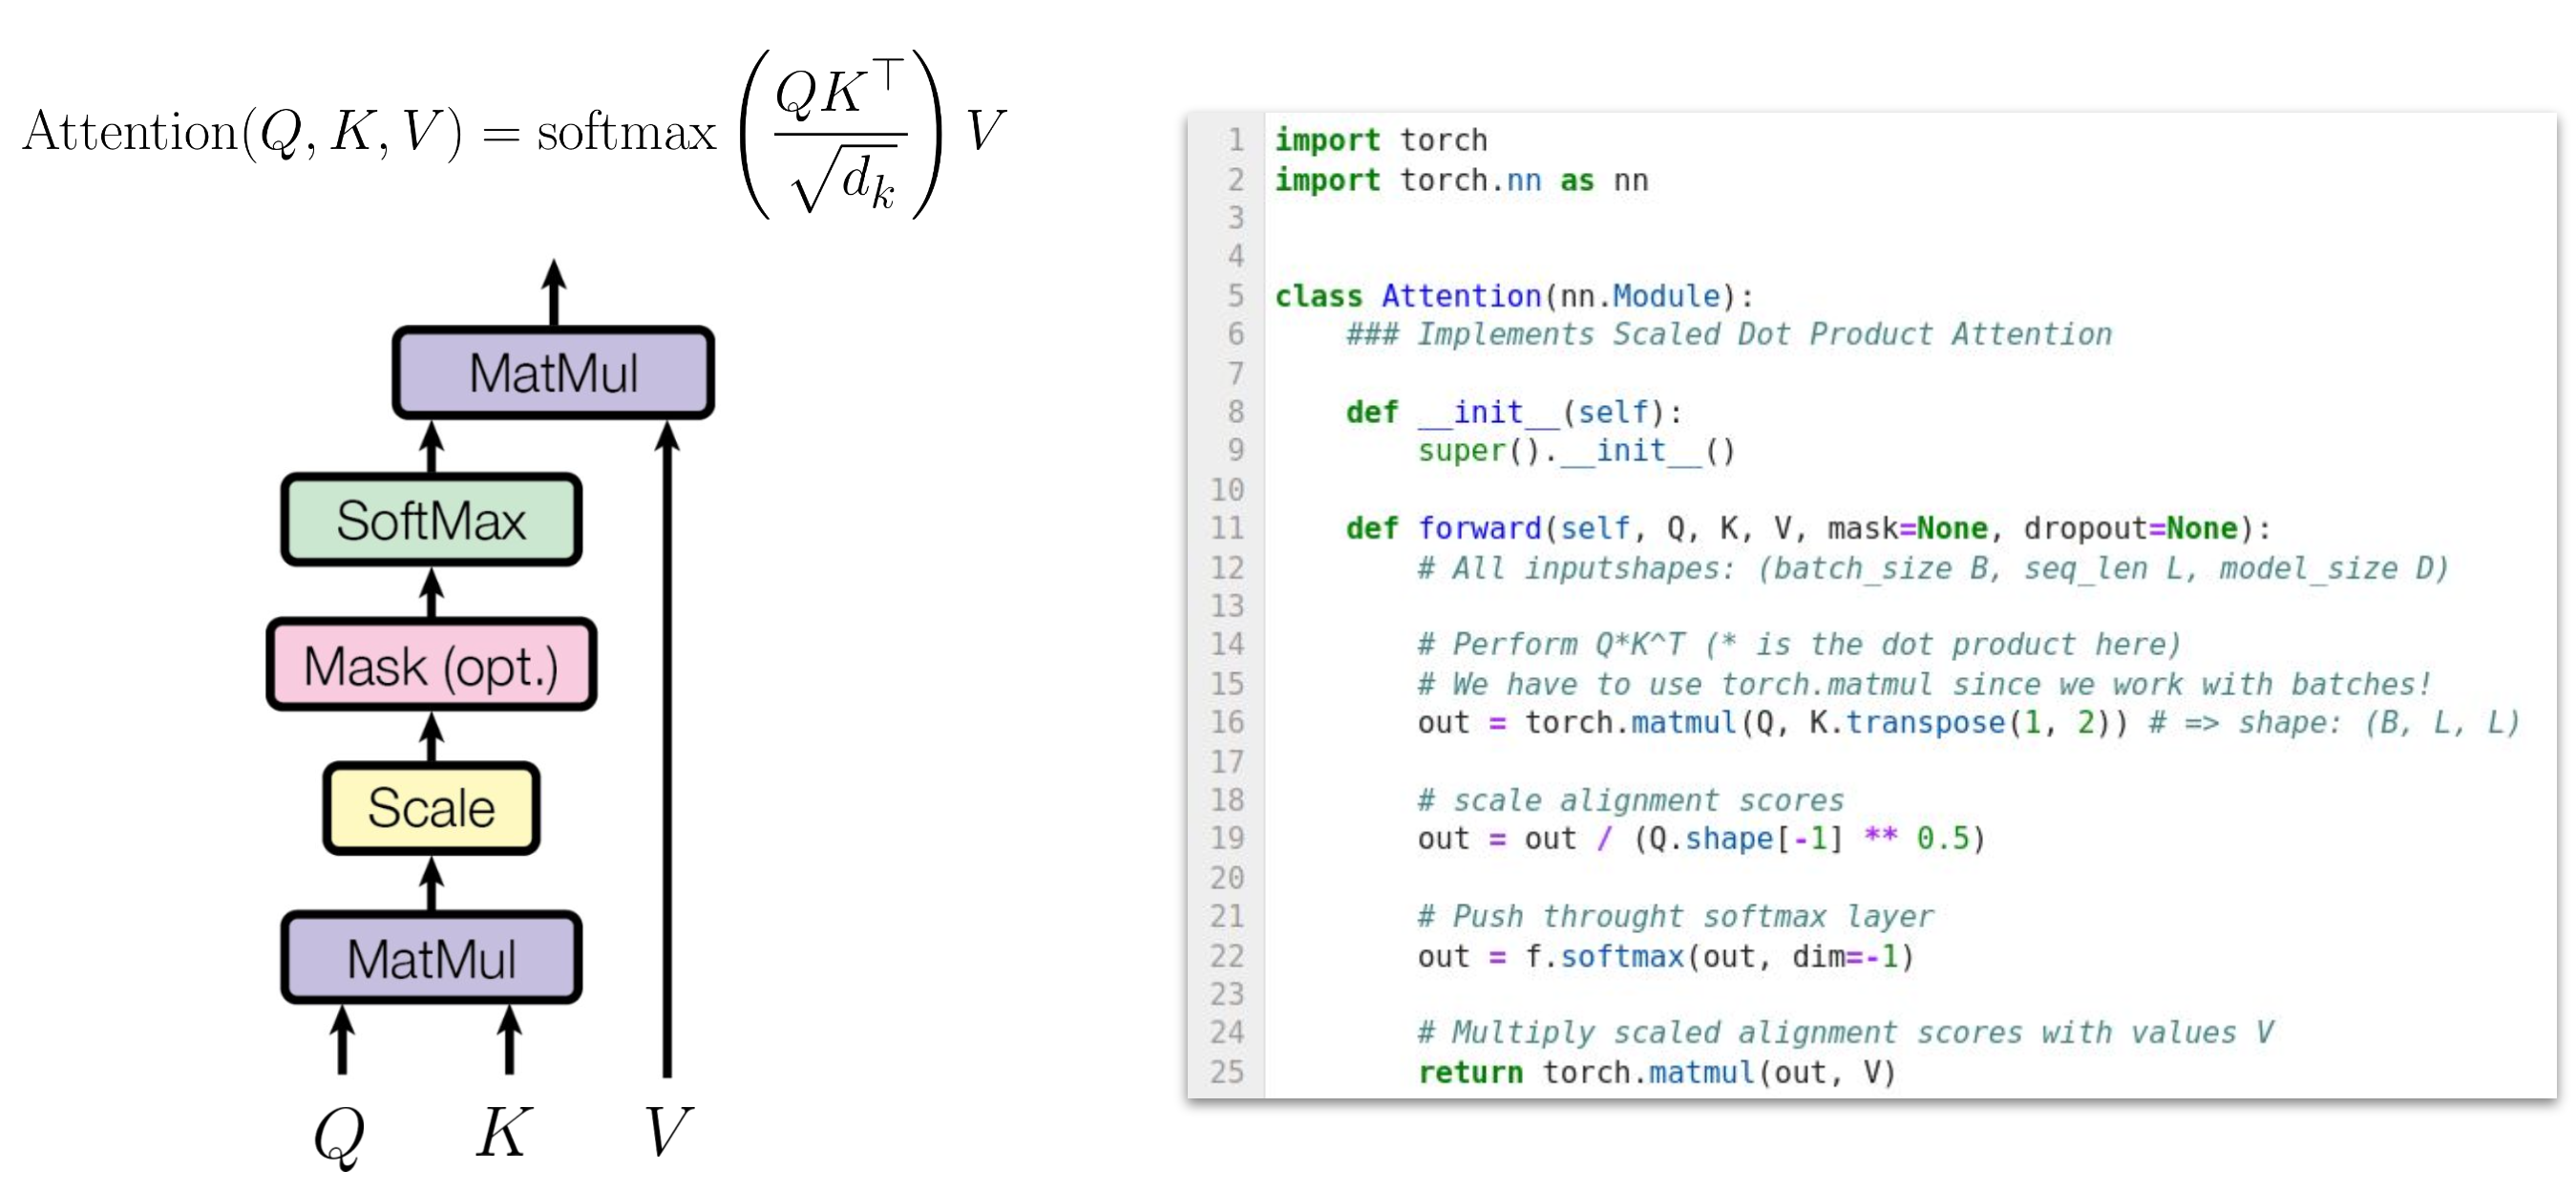
\includegraphics[width=\linewidth]{cs4248-transformer-dotproduct-attention.png}
    \item \textbf{Attention Head}:
    \item \begin{itemize}
      \item Maps model size $d_{model}$ to $d_q$, $d_k$ and $d_v$.
      \item Proposed: $d_q = d_k = d_v = d_{model}/h$.
    \end{itemize}
    \item \textbf{Multi-Head Attention}: The linear layer "unifies" all heads into one. nn.Linear($h \times d_q/d_k/d_v$, $d_{model}$)
    \item \textbf{Feed Forward}: $d_{model} \to d_{hidden} \to d_{model}$
  \end{itemize}
  \subsection{Decoder}
  \begin{itemize}
    \item 2 MHA blocks: one for self-attention and one for cross-attention.
    \item 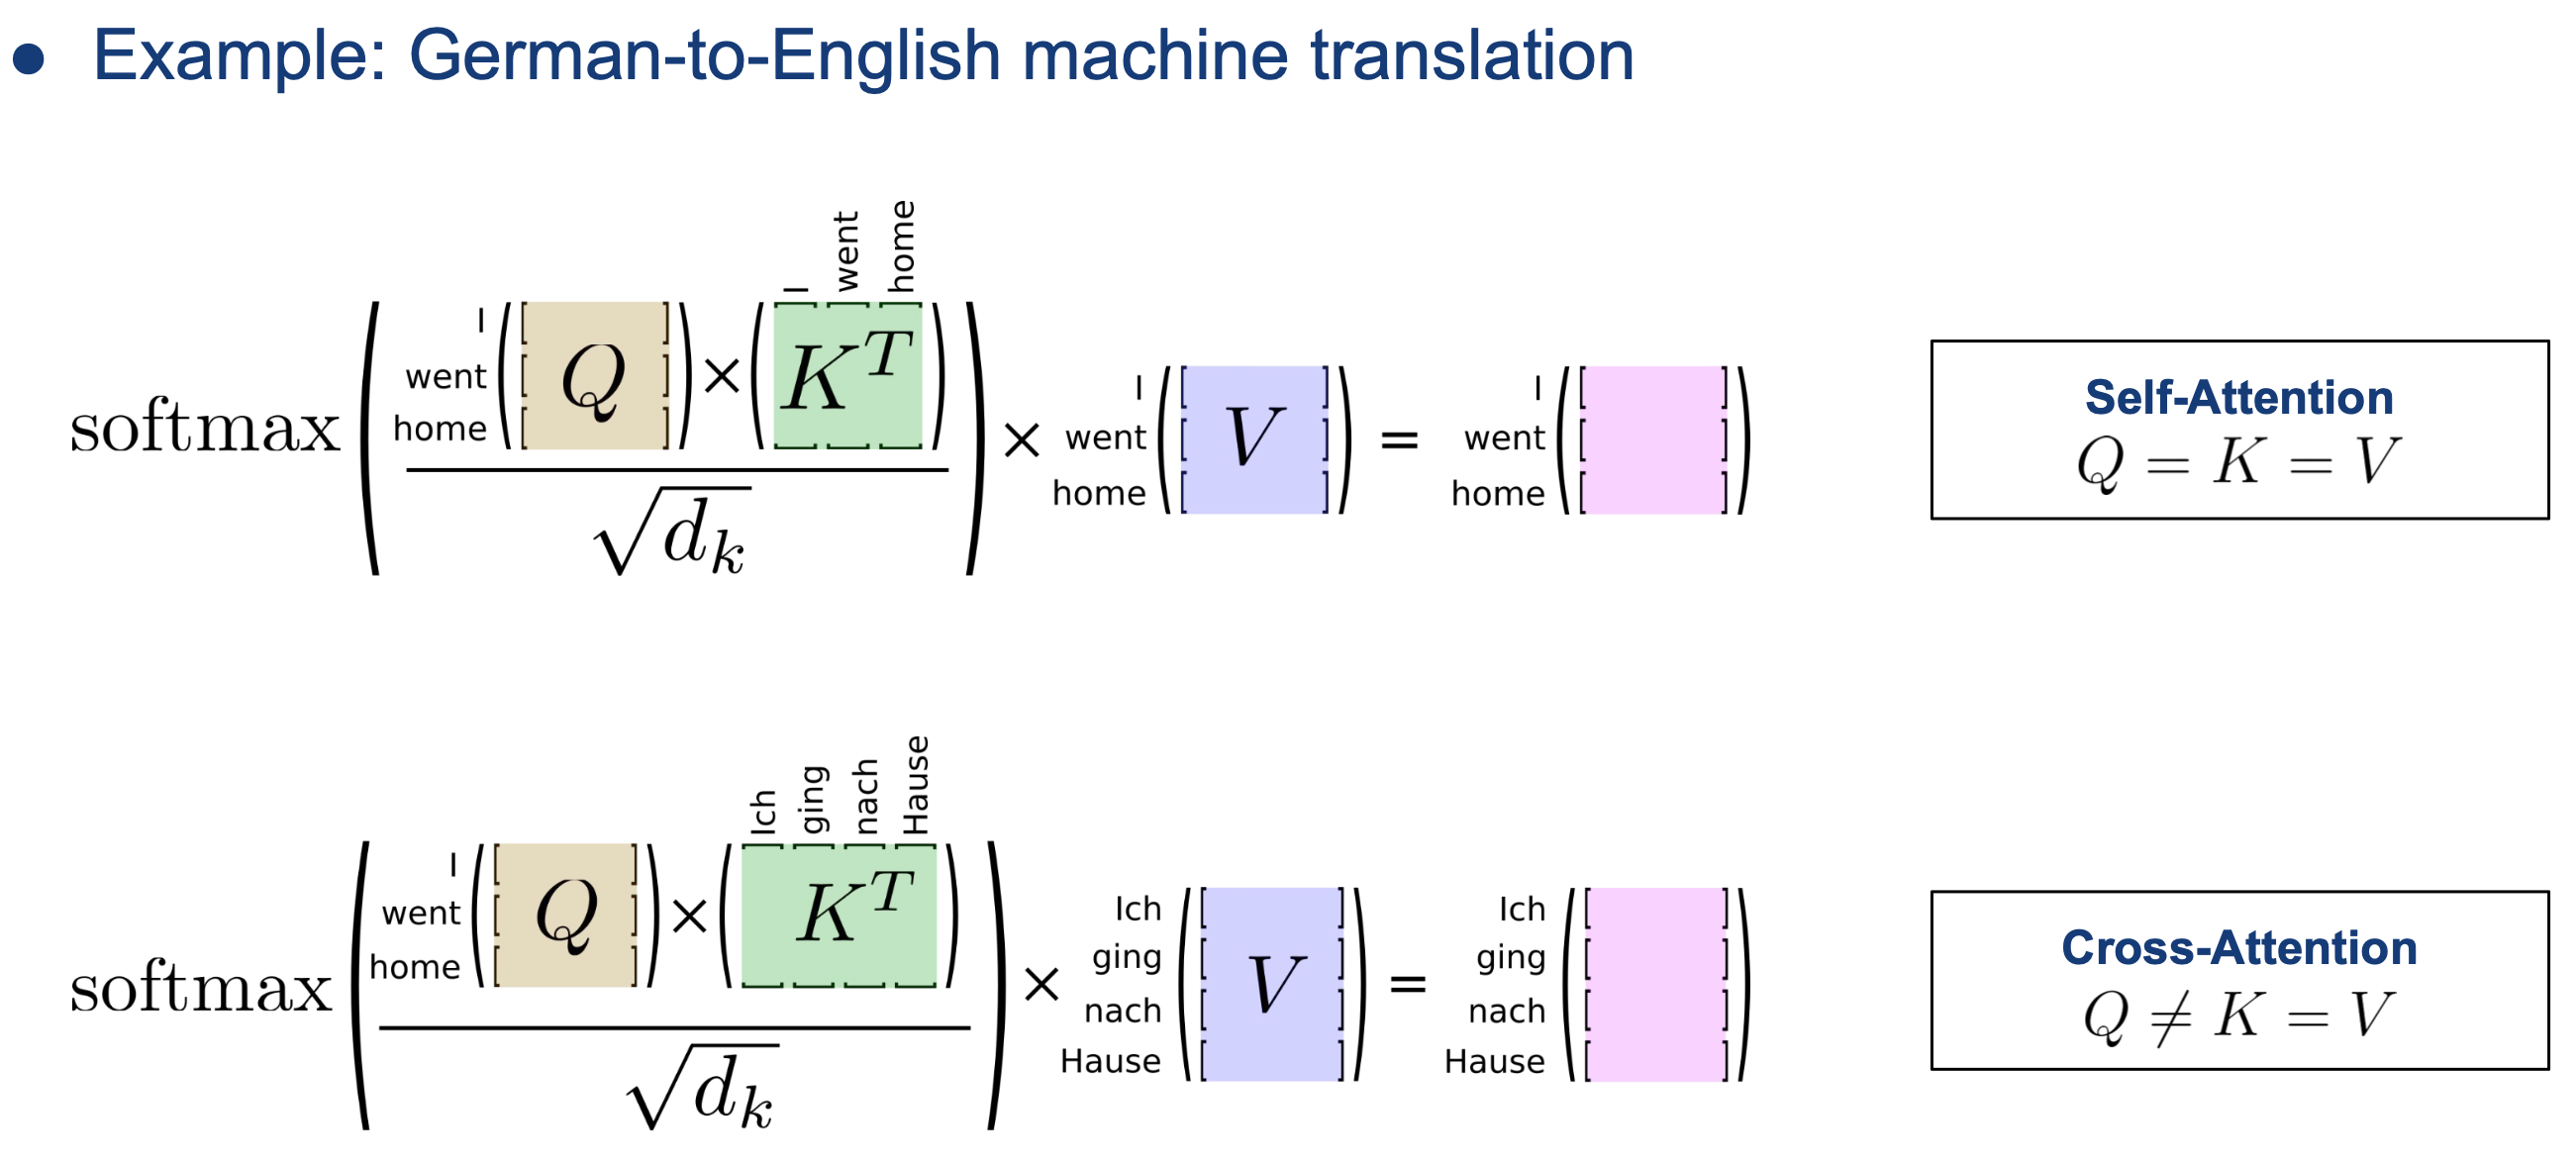
\includegraphics[width=\linewidth]{cs4248-transformer-cross-attention.png}
  \end{itemize}
  \subsubsection{Masking}
  \begin{itemize}
    \item Purpose: Ignore \textless PAD\textgreater, "hidden" words and future words.
    \item Mask "hidden" words: Train the model to predict the hidden words.
    \item \textbf{Mask future words}: "Causal masking" to prevent the model from seeing future words, in autoregressive training.
  \end{itemize}
  \subsubsection{Restricted attention}
  \begin{itemize}
    \item \textbf{Sparse attention}: only attend to a subset of the input sequence, to make the number of computations $O(n)$.
    \item 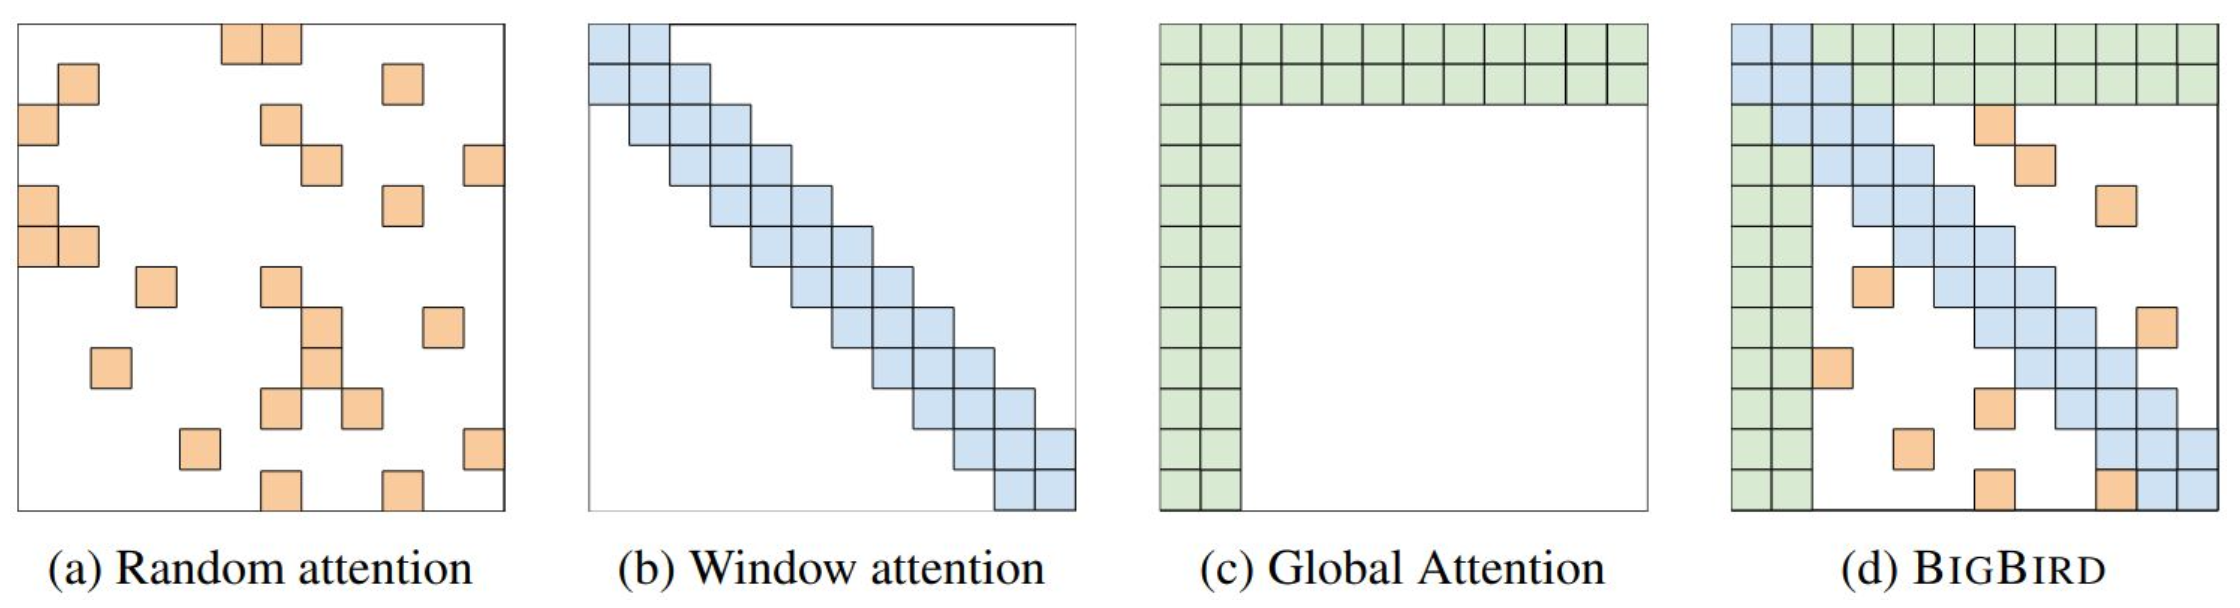
\includegraphics[width=\linewidth]{cs4248-transformer-sparse-attention.png}
    \item Other approaches include:
    \item \begin{itemize}
      \item Linear attention: Approximates attention with lower-rank representation.
      \item Flash attention: \dots
      \item Selective routing: Attend to most relevant tokens.
    \end{itemize}
  \end{itemize}
  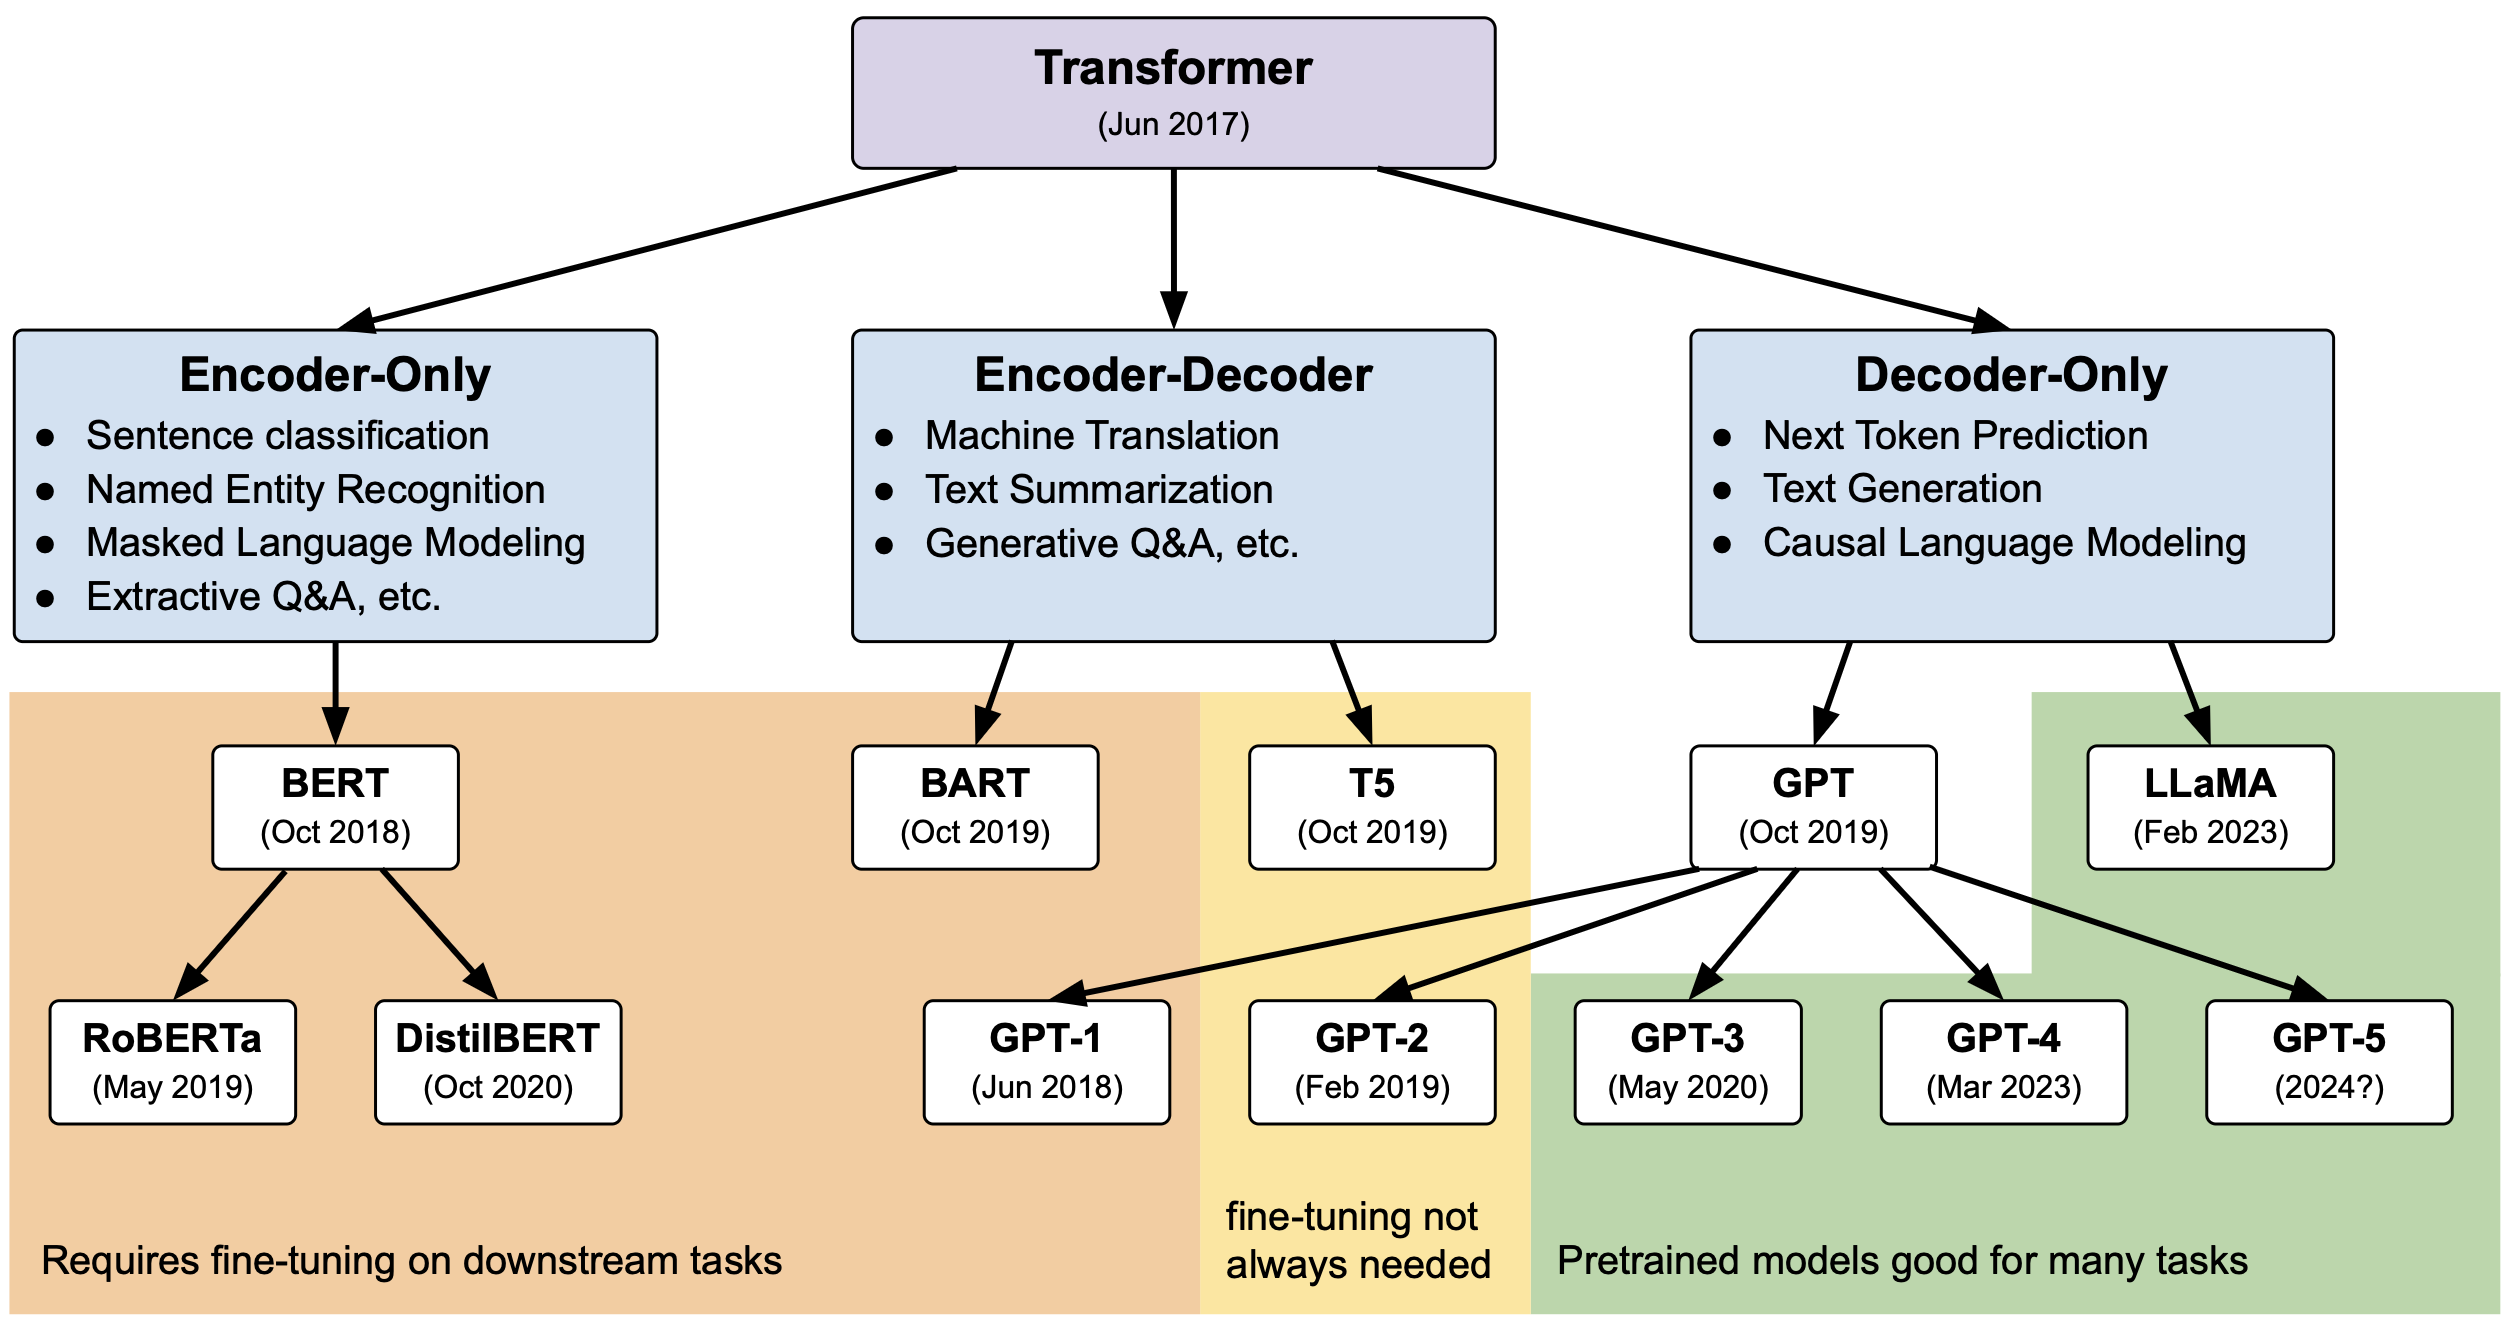
\includegraphics[width=\linewidth]{cs4248-transformer-categories.png}

  \section{11 - LLMs}
  \subsection{Encoder-only}
  \subsubsection{BERT}
  \begin{itemize}
    \item Uses only the transformer encoder, self-supervised training.
    \item Trained on 2 tasks: Masked language modeling (MLM) and next sentence prediction (NSP, a \textit{binary classification} task).
  \end{itemize}
  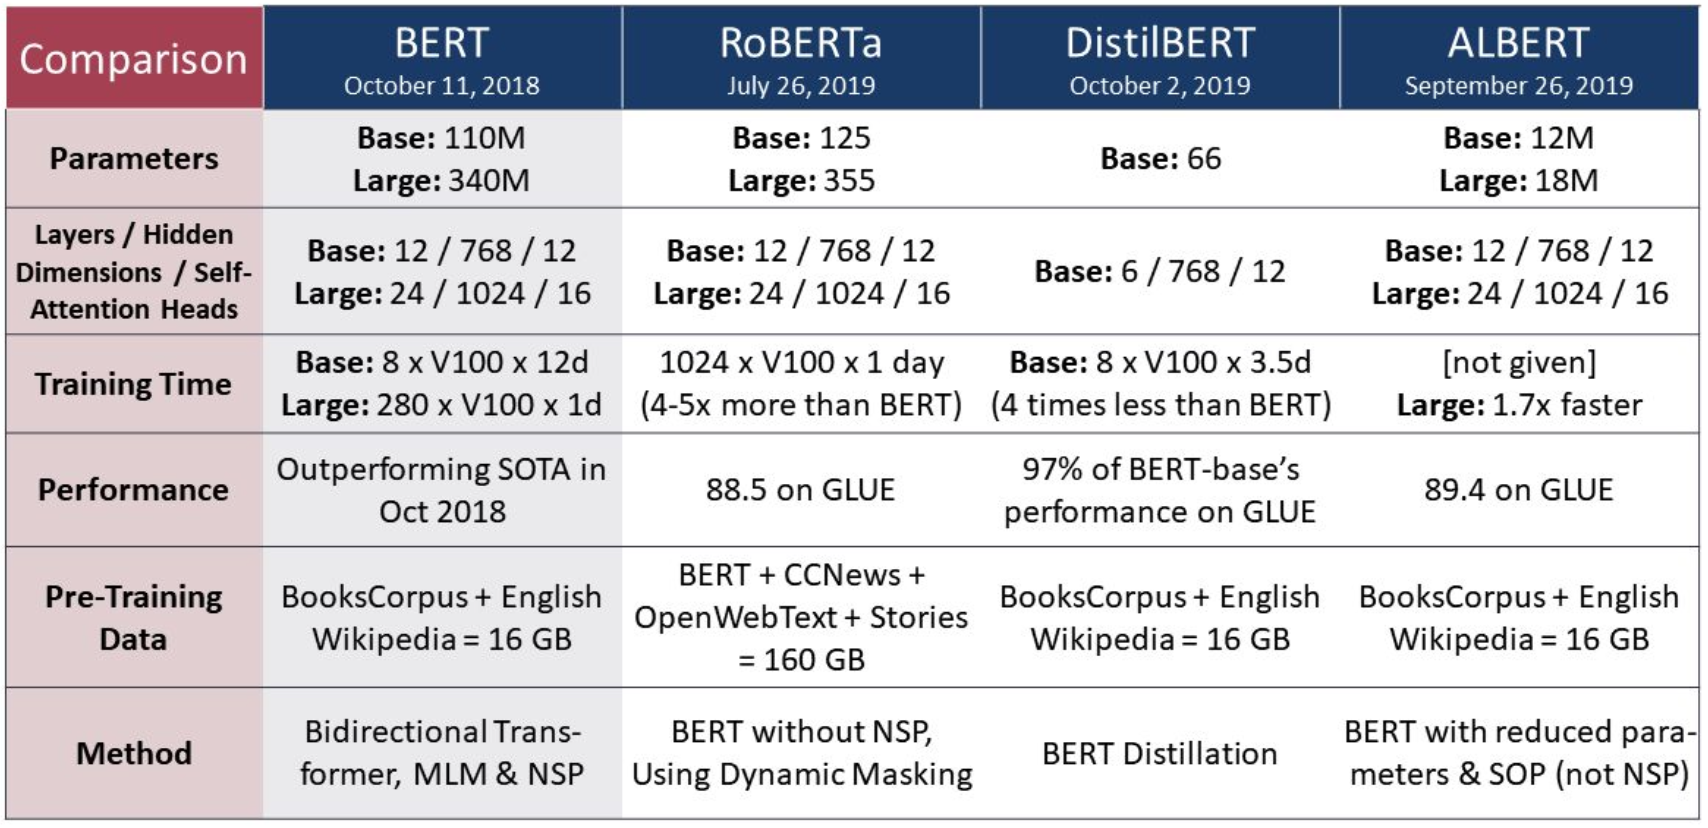
\includegraphics[width=\linewidth]{cs4248-llm-bert-family.png}
  \begin{itemize}
    \item Model distillation: Task the student model to predict the entire probability distribution of the teacher model output.
  \end{itemize}

  \subsection{Encoder-decoder}
  \subsubsection{T5}
  \begin{itemize}
    \item Multi-task learning: model training on multiple tasks simultaneously (e.g., machine translation, coreference resolution, text summarization, sentence acceptability judgment, sentiment analysis)
    \item Each task is (re-)formulated as text-to-text task to match the encoder-decoder architecture (adding task-specific prefixes).
  \end{itemize}
  \subsubsection{BART}
  \begin{itemize}
    \item Trained by corrupting documents and then optimizing a reconstruction loss, i.e. denoising (the cross-entropy between the decoder's output and the original document)
    \item "Multi-task via augmentation": e.g. token masking, sentence permutation, document rotation, etc.
  \end{itemize}
  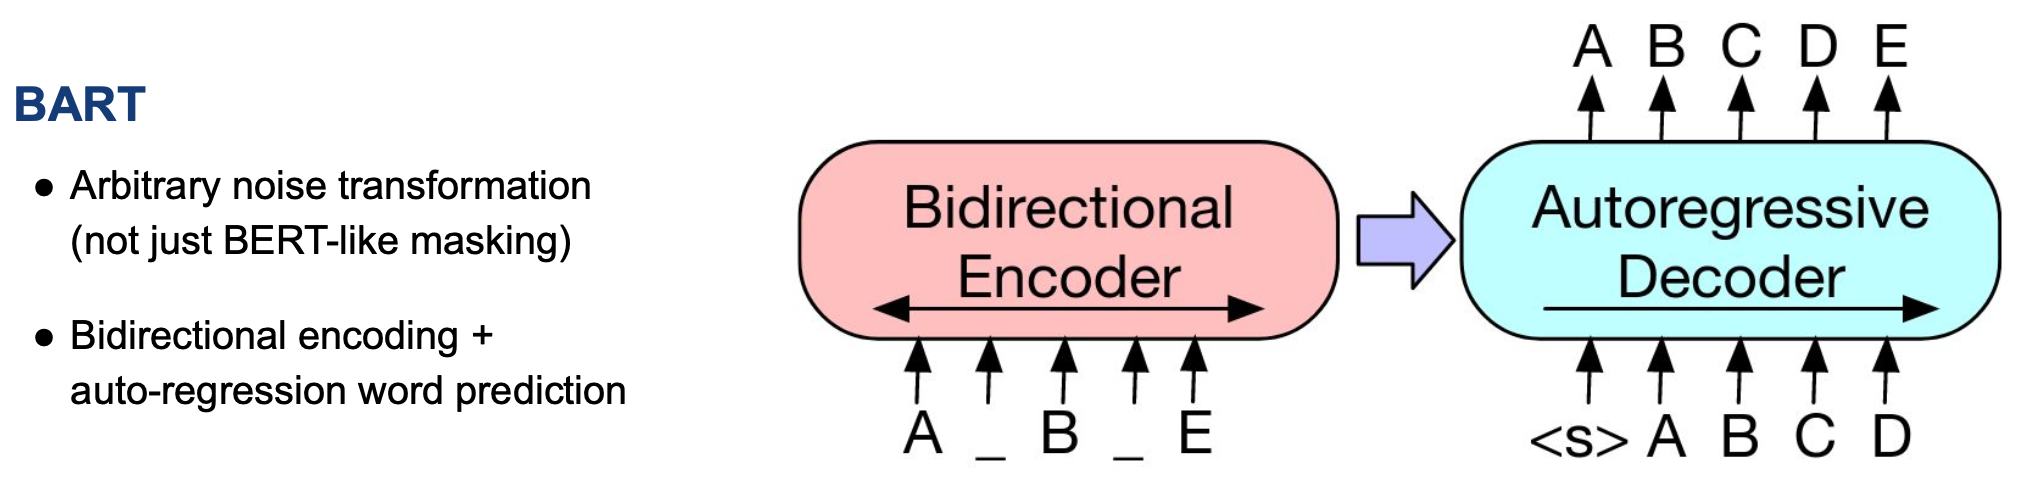
\includegraphics[width=\linewidth]{cs4248-llm-bart.png}

  \subsection{Decoder-only}
  \subsubsection{GPT}
  \begin{itemize}
    \item Uses only the transformer decoder, autoregressive training.
    \item ChatGPT-1/2/3: text only, “just” making it larger; GPT-4: multimodal.
    \item ChatGPT-3+: reinforcement learning from human feedback (RLHF).
    \item \textbf{RLHF}: Use human-generated responses to prompts to fine-tune the pretrained model.
  \end{itemize}
  \subsubsection{LLaMA}
  \begin{itemize}
    \item Pre-normalization: layer normalization is put inside the residual blocks.
    \item 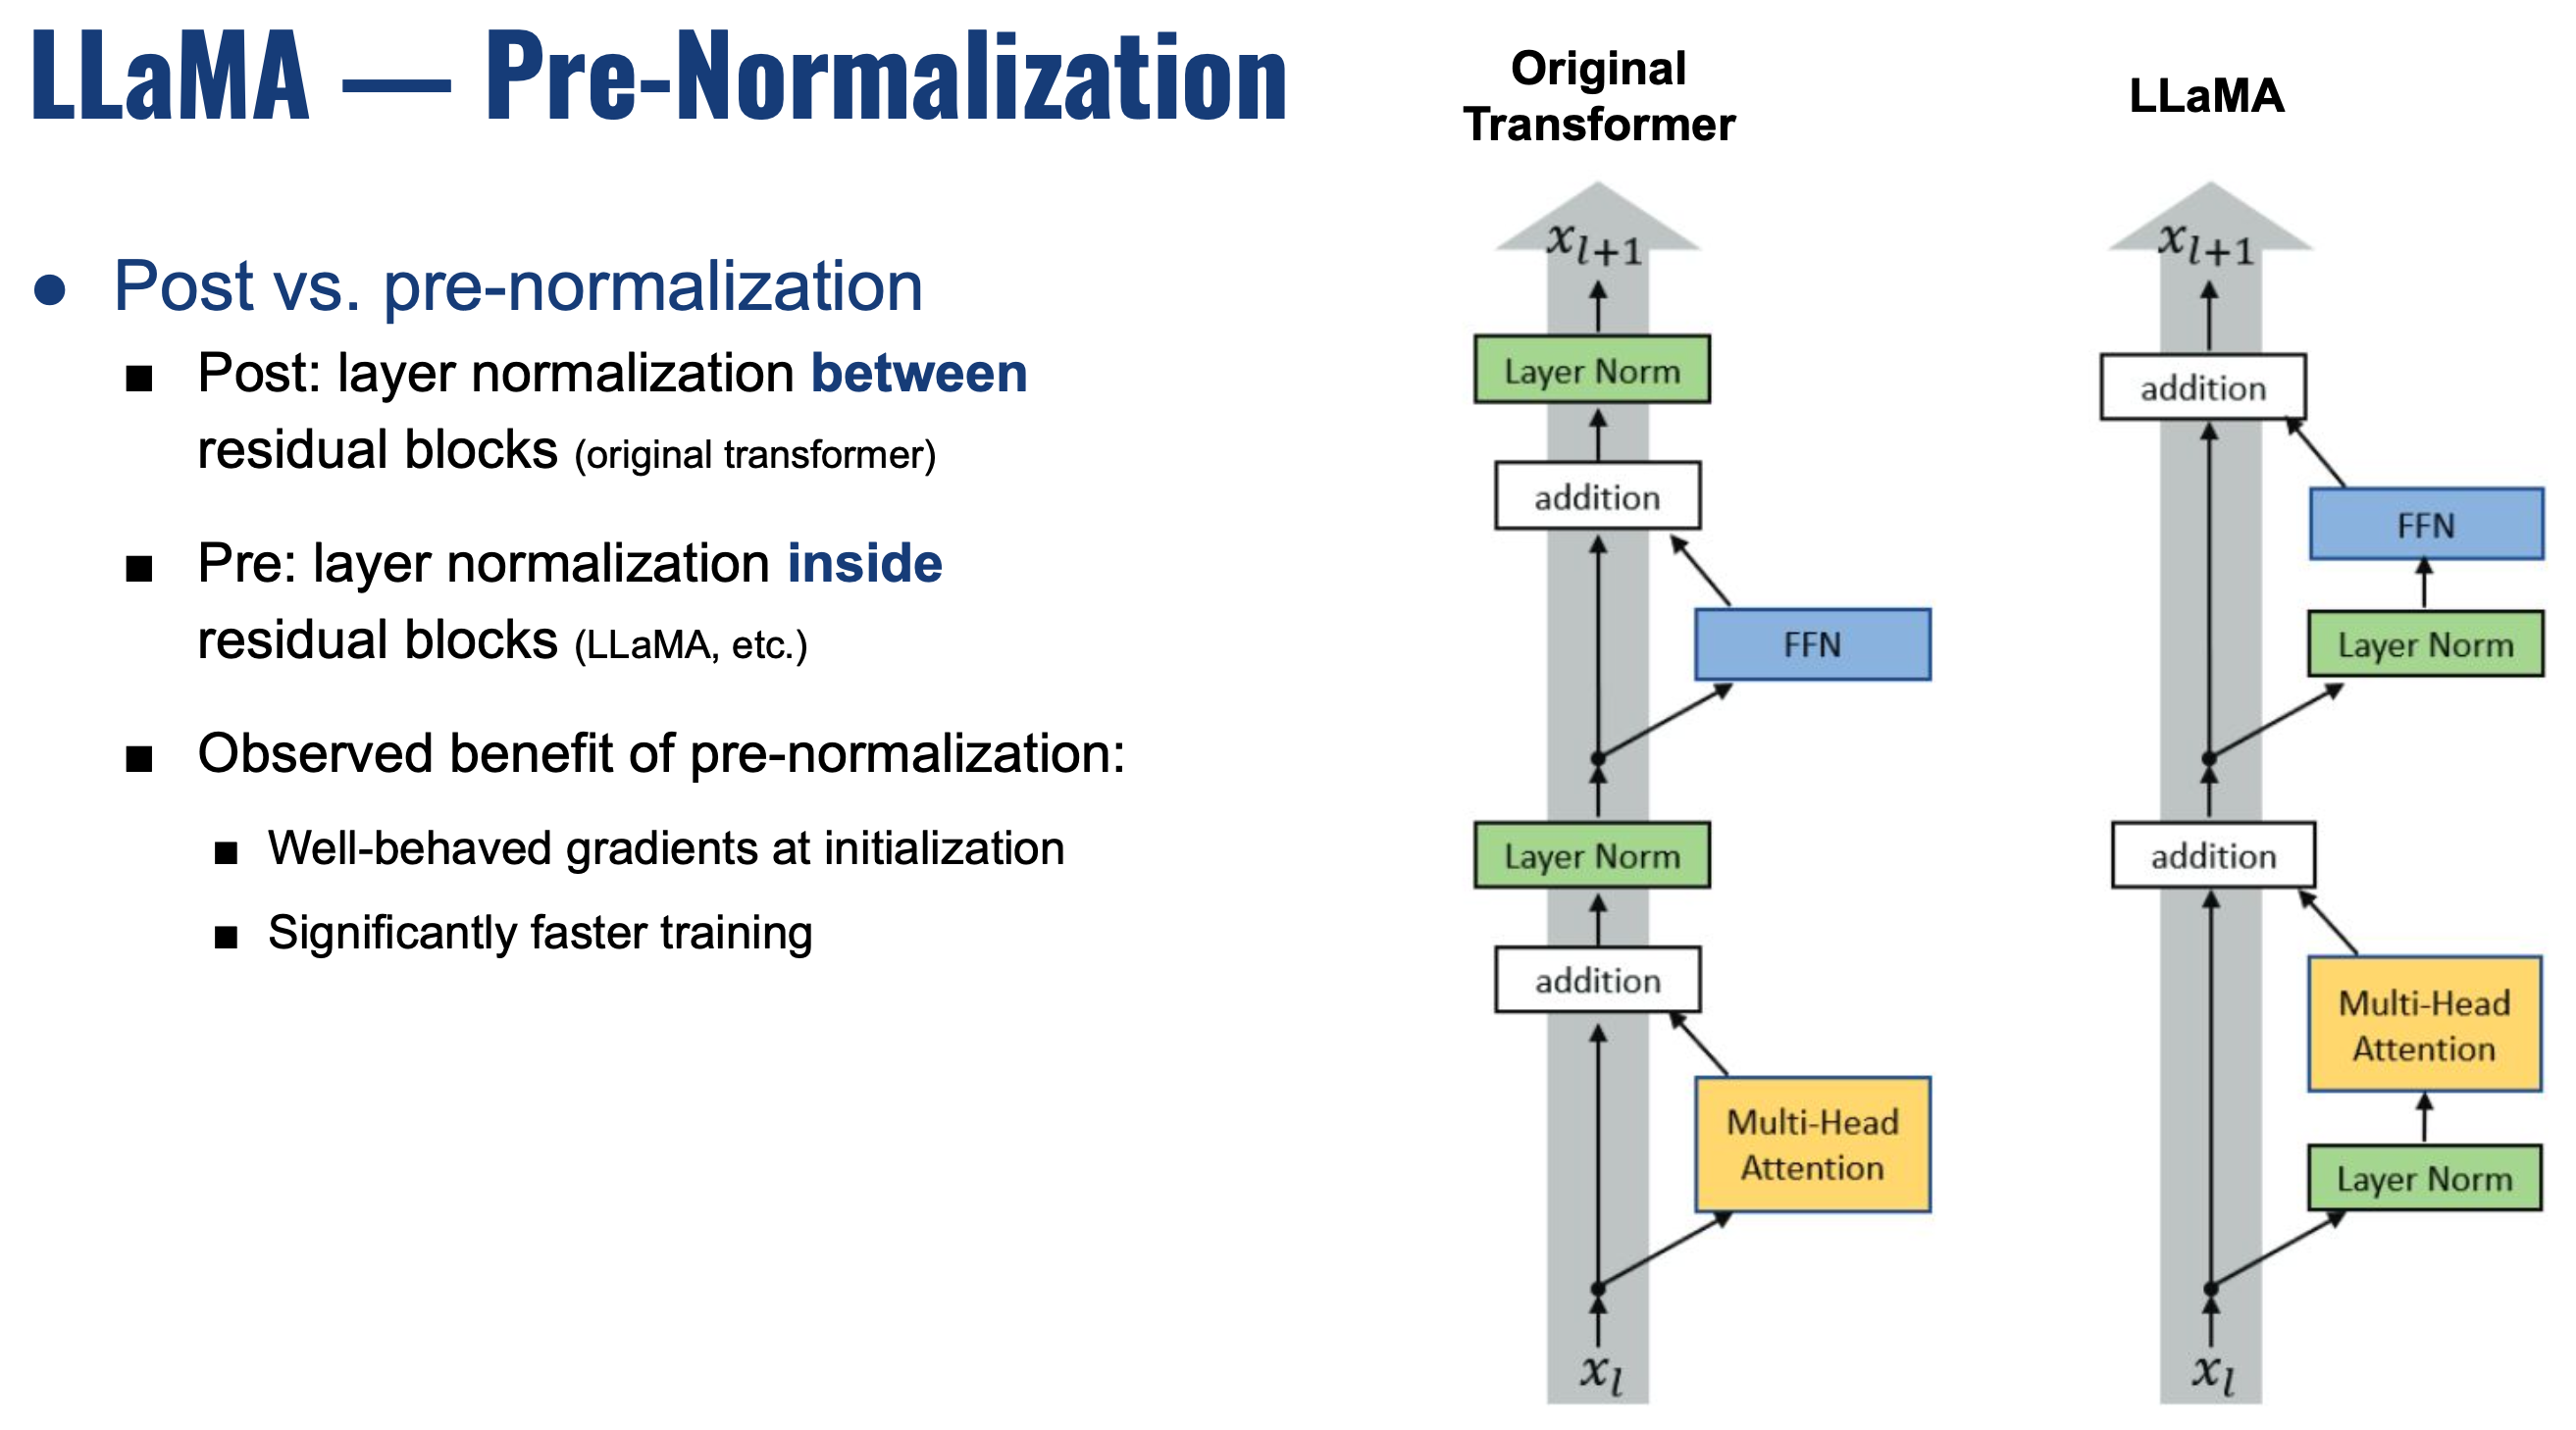
\includegraphics[width=\linewidth]{cs4248-llm-llama-prenorm.png}
    \item SwiGLU (Swish-Gated Linear Unit) activation: non-monotonic, parameterized activation function.
    \item Rotary Positional Embeddings (RoPE): encode word positions by rotating word embedding vectors.
    \item Open LLM: Trained exclusively on
    publicly available data.
  \end{itemize}

  \subsection{Limitations and challenges}
  \begin{itemize}
    \item Inferencing cost: Image generation is the highest.
    \item Model alignment: Aligns with users' preferences and moral compass.
    \item Accuracy/hallucination, Misinformation/disinformation/fake news, Prompted-based jailbreaking (e.g. pretending).
  \end{itemize}

  \subsection{Prompt engineering}
  \begin{itemize}
    \item Definition: The practice of designing and optimizing prompts to elicit desired responses from LLMs.
    \item 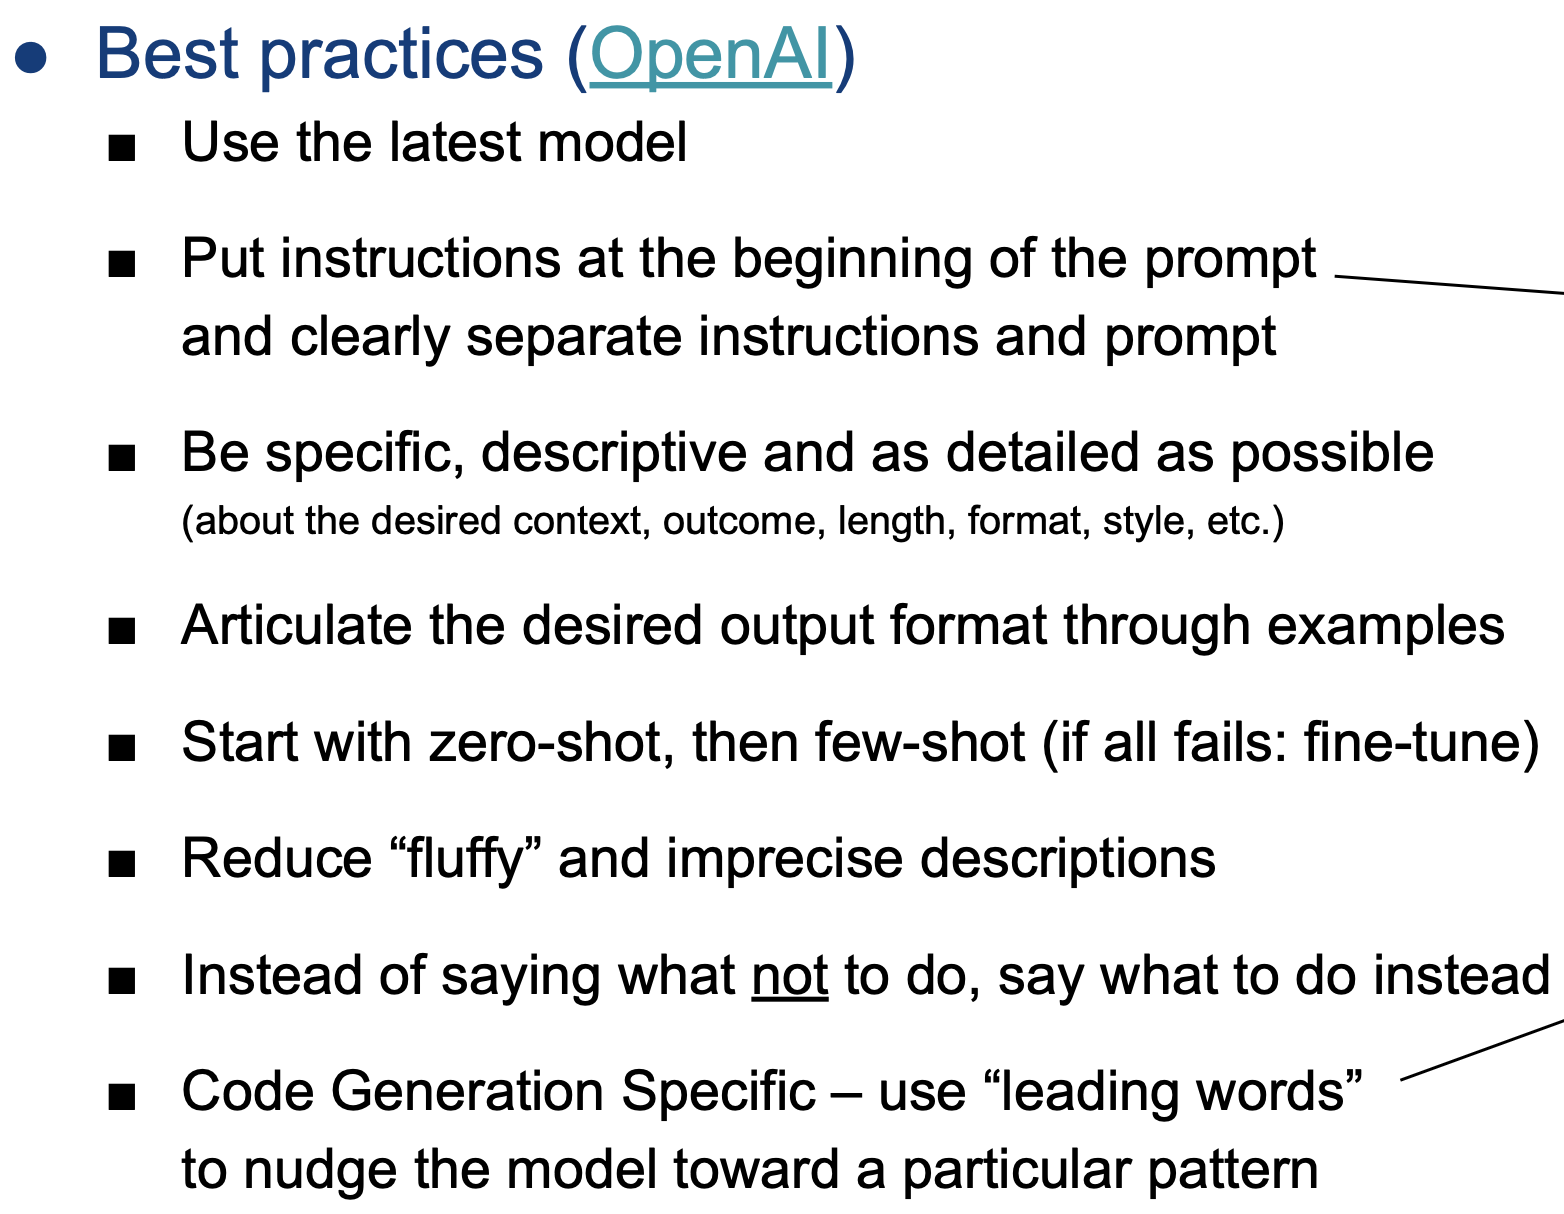
\includegraphics[width=0.4\linewidth]{cs4248-llm-prompt-engi.png} 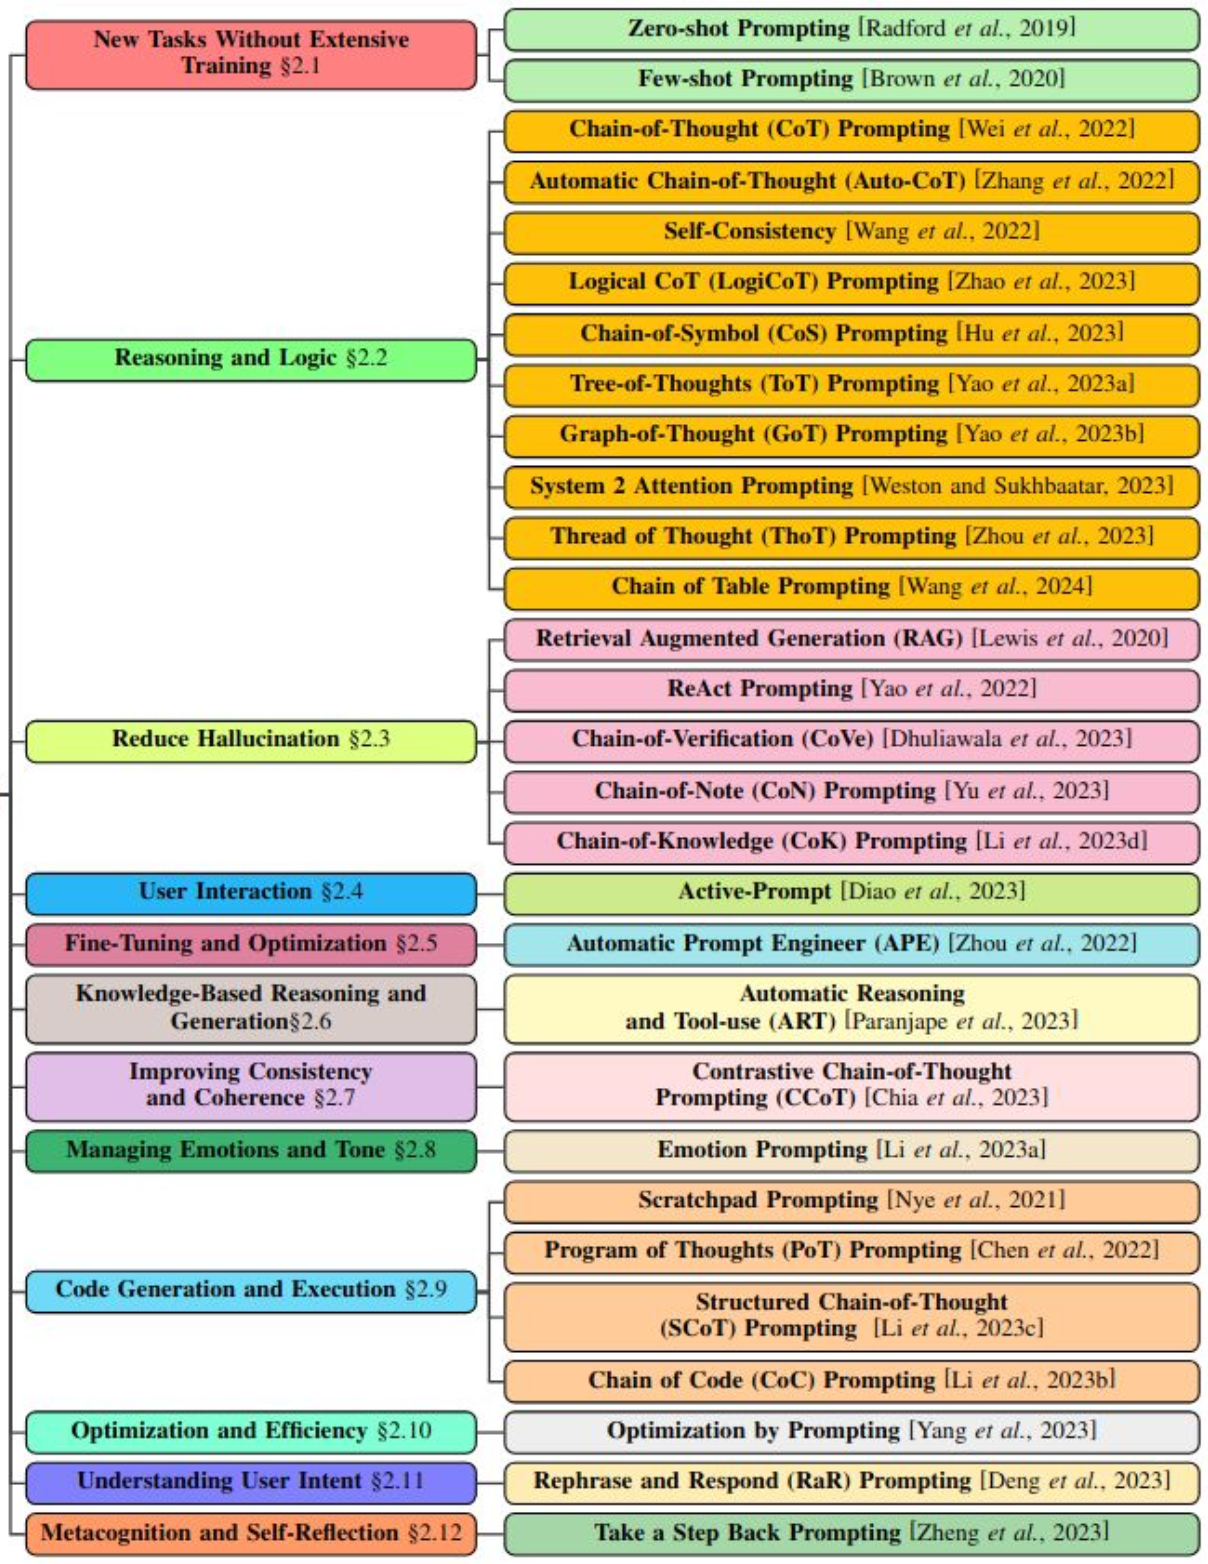
\includegraphics[width=0.55\linewidth]{cs4248-llm-prompt-engi-2.png}
    \item \textbf{X-shot prompting}: zero-shot, one-shot, few-shot \textrightarrow In-context learning (ICL).
    \item \textbf{In-context learning}:
    \item \begin{itemize}
      \item Intuition: Demonstrations help to "locate" latent concepts acquired during pre-training.
      \item Observation 1: Correctness of the demonstration label is not important.
      \item Observation 2: More demonstrations help up to a certain threshold.
      \item Observation 3: Relevance of demonstrations is important.
      \item Observation 4: Label space matters.
      \item Observation 5: Order of demonstrations and distribution of labels matter.
    \end{itemize}
    \item \textbf{RAG}:
    \item \begin{itemize}
      \item Retrieve relevant snippets of knowledge (chunks) and add as context to prompt.
      \item Benefits: Grounding of LLM responses on (hopefully) factual data, simple integration of (very) recent and/or very domain-specific data, improved transparency, customization/personalization.
      \item \textbf{Chunking}: External data needs to be splitted into "meaningful" chunks of practical sizes.
      \item \begin{itemize}
        \item Fixed size chunking.
        \item Recursive chunking: top-down approach to keep paragraphs/sentences intact as much as possible.
        \item Document-based chunking: utilize document structure: Markdown headings, tables, source code, etc.
        \item Semantic chunking: chunk = group of sentences based on their embedding similarities.
        \item Agentic chucking: novel idea: let the LLM decide where to best split.
      \end{itemize}
      \item \textbf{Storing and retrieval}:
      \item \begin{itemize}
        \item "Classic" IR: Store chunks as text documents, index (text\textrightarrow document) and query with prompts.
        \item Vector database retrieval: Embed chunks and store embedding vectors. Index the vectors. Embed prompt and search for nearest vectors.
        \item Common goals: Store large volumes and support fast access.
      \end{itemize}
    \end{itemize}
  \end{itemize}

  \subsection{Fine-tuning}
  \subsubsection{Prompt tuning}
  \begin{itemize}
    \item Automatically learn the context for a given task.
    \item Approach: context = trainable embedding vector
  \end{itemize}
  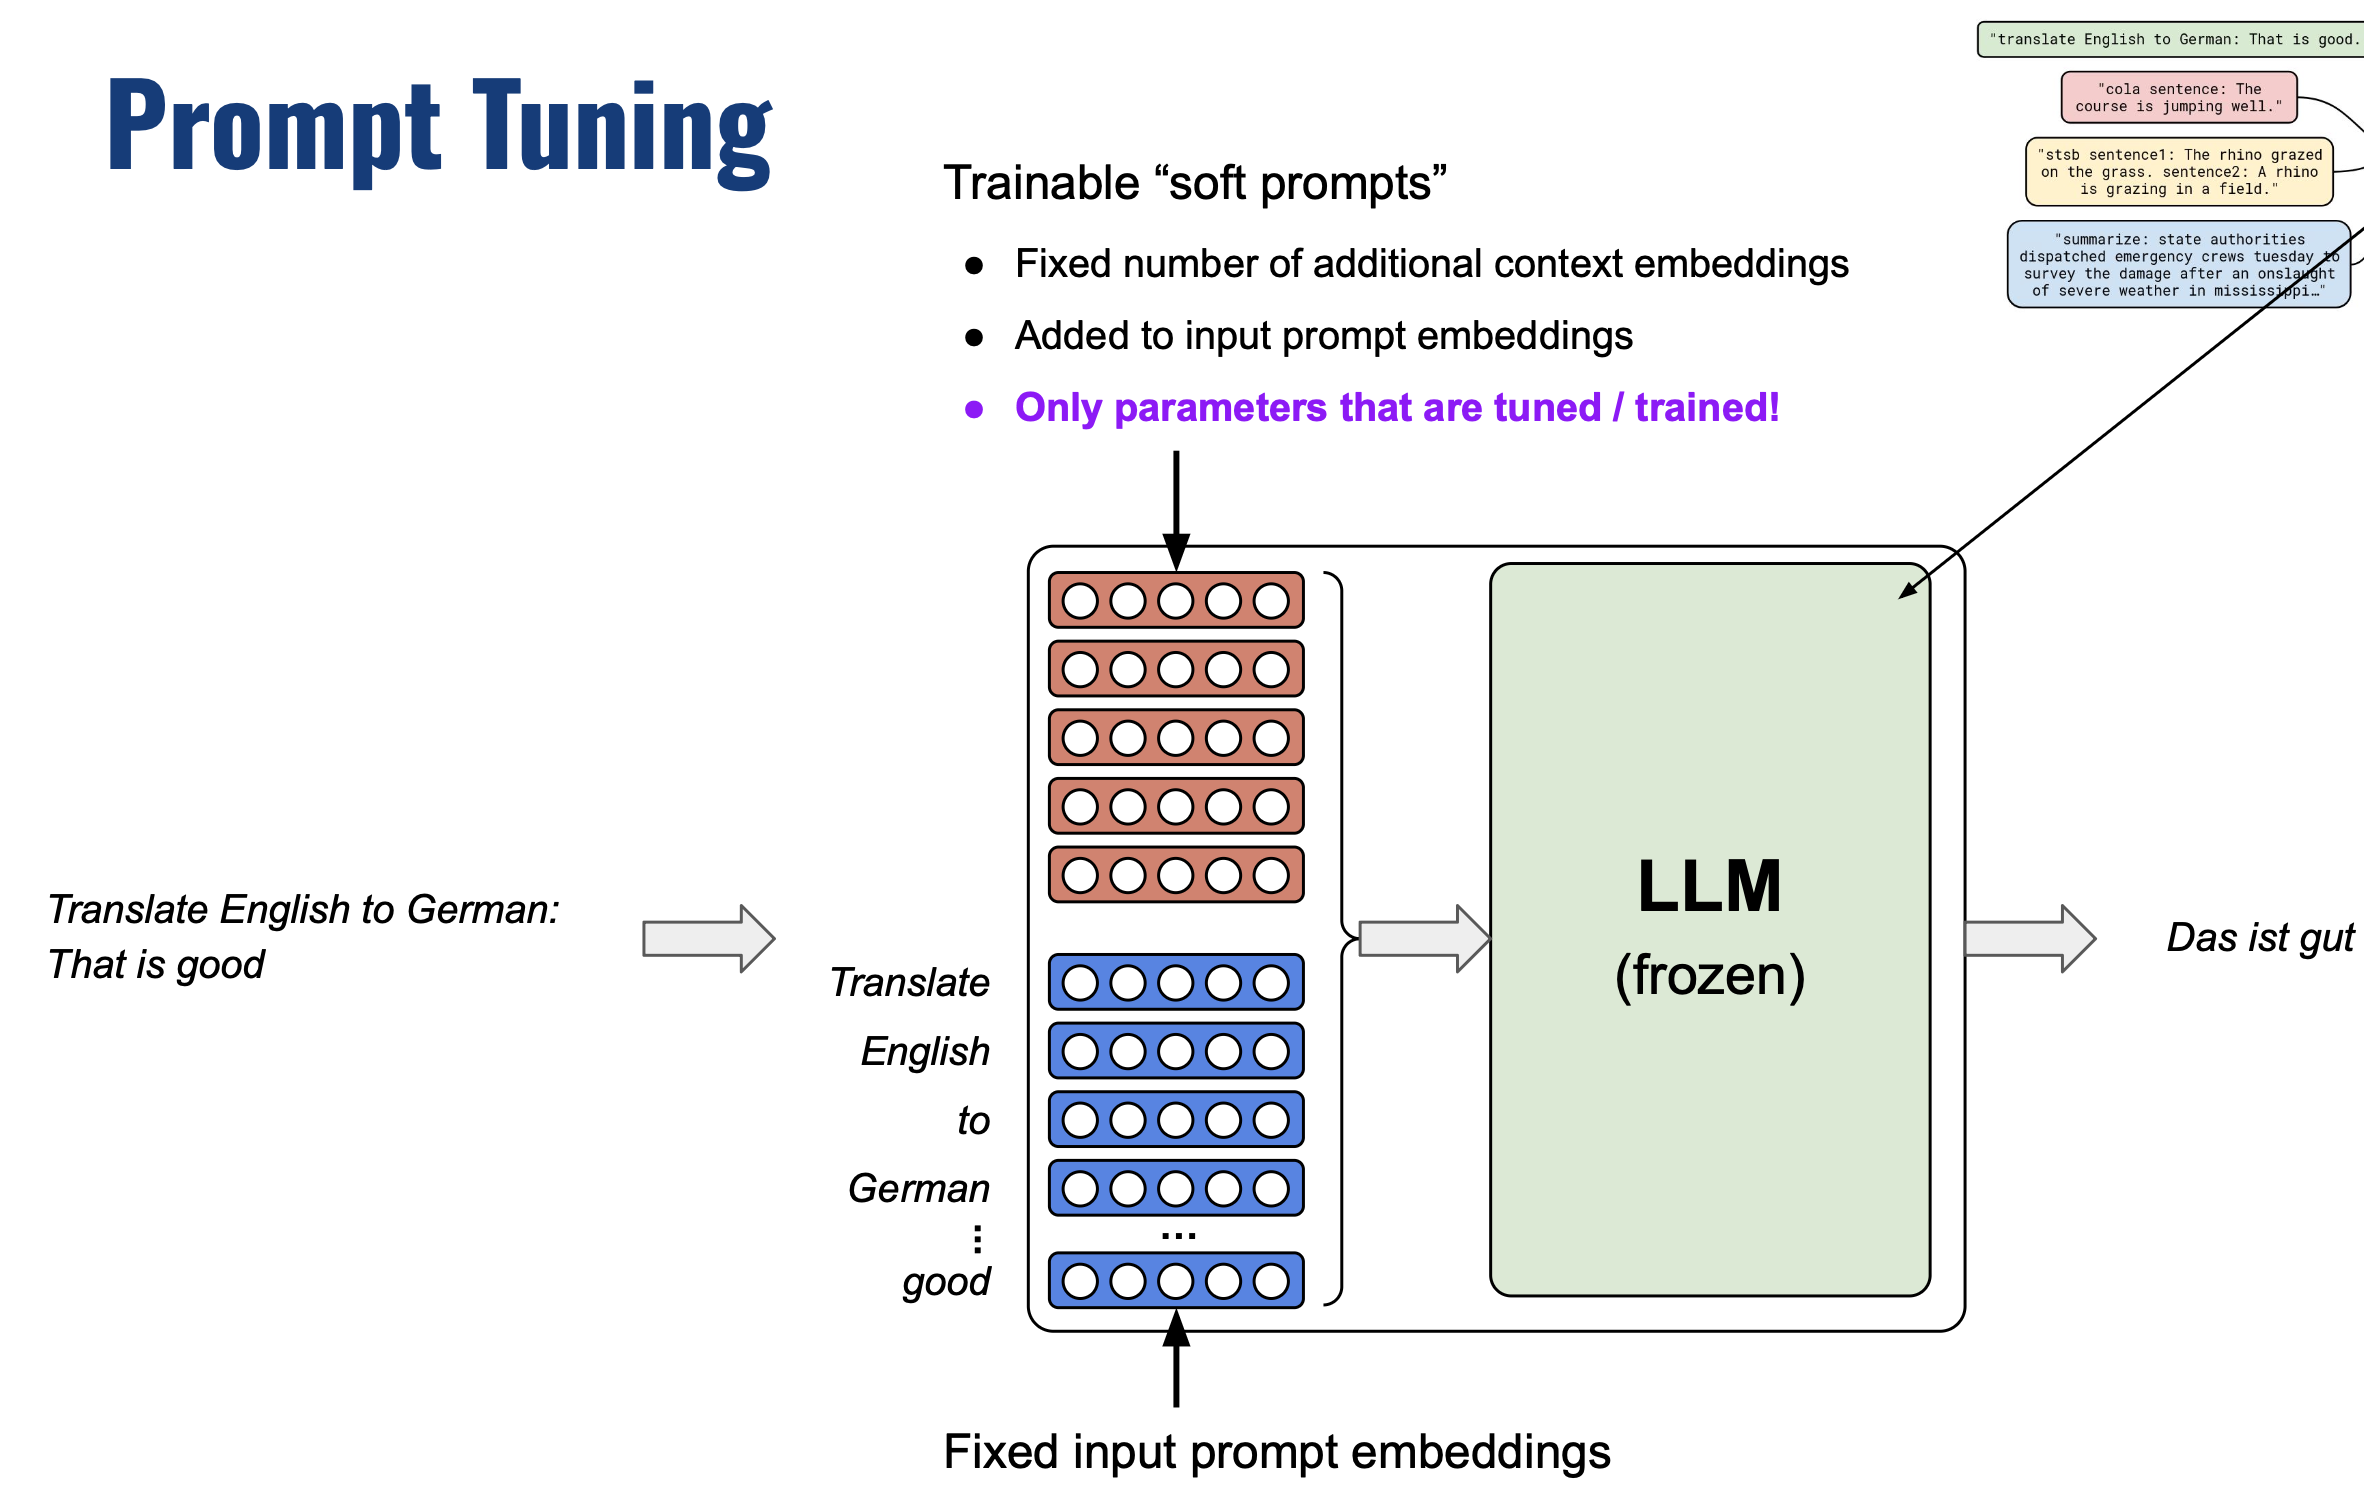
\includegraphics[width=\linewidth]{cs4248-llm-prompt-tuning.png}
  \subsubsection{Prefix tuning}
  \begin{itemize}
    \item Add small number of trainable vectors to \textbf{each transformer block}.
    \item Different additional vectors for different tasks (can be swapped out during inferencing).
  \end{itemize}
  \subsubsection{LoRA}
  \begin{itemize}
    \item Mismatch: training objective (next-word prediction) vs. user's objective (task-specific).
    \item Common data setup: Instruction fine-tuning: custom instruction dataset with (instruction, output)-pairs.
    \item Parameter-efficient fine-tuning: only train a small number of parameters.
    \item \textbf{LoRA}: Low-Rank Adaptation
    \item Adapter: small, trainable module added to a pretrained network model. Low-rank approximation of the weight matrix.
    \item \textbf{Why does it work}? Weight matrices often reside within low-rank spaces, hence smaller matrices would suffice. (e.g. explained variance remains high after dimensionality reduction).
    \item Benefits: 
    \item \begin{itemize}
      \item Flexibility: LoRA can be applied to all or only some weight matrices.
      \item Less trainable parameters/weights: Lower memory requirements, faster training.
      \item Pretrained weights remain unchanged: Preserving original model's quality.
    \end{itemize}
    \item Drawbacks:
    \item \begin{itemize}
      \item Increased complexity: Adding LoRA to existing model is not trivial.
      \item Performance: LoRA might not perform as well as full fine-tuning.
    \end{itemize}
  \end{itemize}
  \subsubsection{Data preparation}
  \begin{itemize}
    \item Irrelevant data: HTML skeletons, \dots
    \item Low-quality data: GPT-2 approach: crowdsourcing of quality control.
    \item Duplicate data: e.g. repeated news articles, \dots
    \item \textbf{Data decontamination}: 
    \item \begin{itemize}
      \item Often not clear which data a non-public LLM was trained on.
      \item No guarantee that a test dataset was not part of the training dataset.
      \item GPT-2 approach: Remove Wikipedia articles from the training dataset. (Wikipedia is commonly used for testing.)
    \end{itemize}
    \item Toxicity and biases: "improper" data, "Model Collapse" (when the training data has content generated by the model itself), \dots
    \item Privacy-sensitive information
  \end{itemize}

  \section{12 - Recent Developments in NLP}
  \begin{itemize}
    \item The efficiency spectrum:
  \end{itemize}
  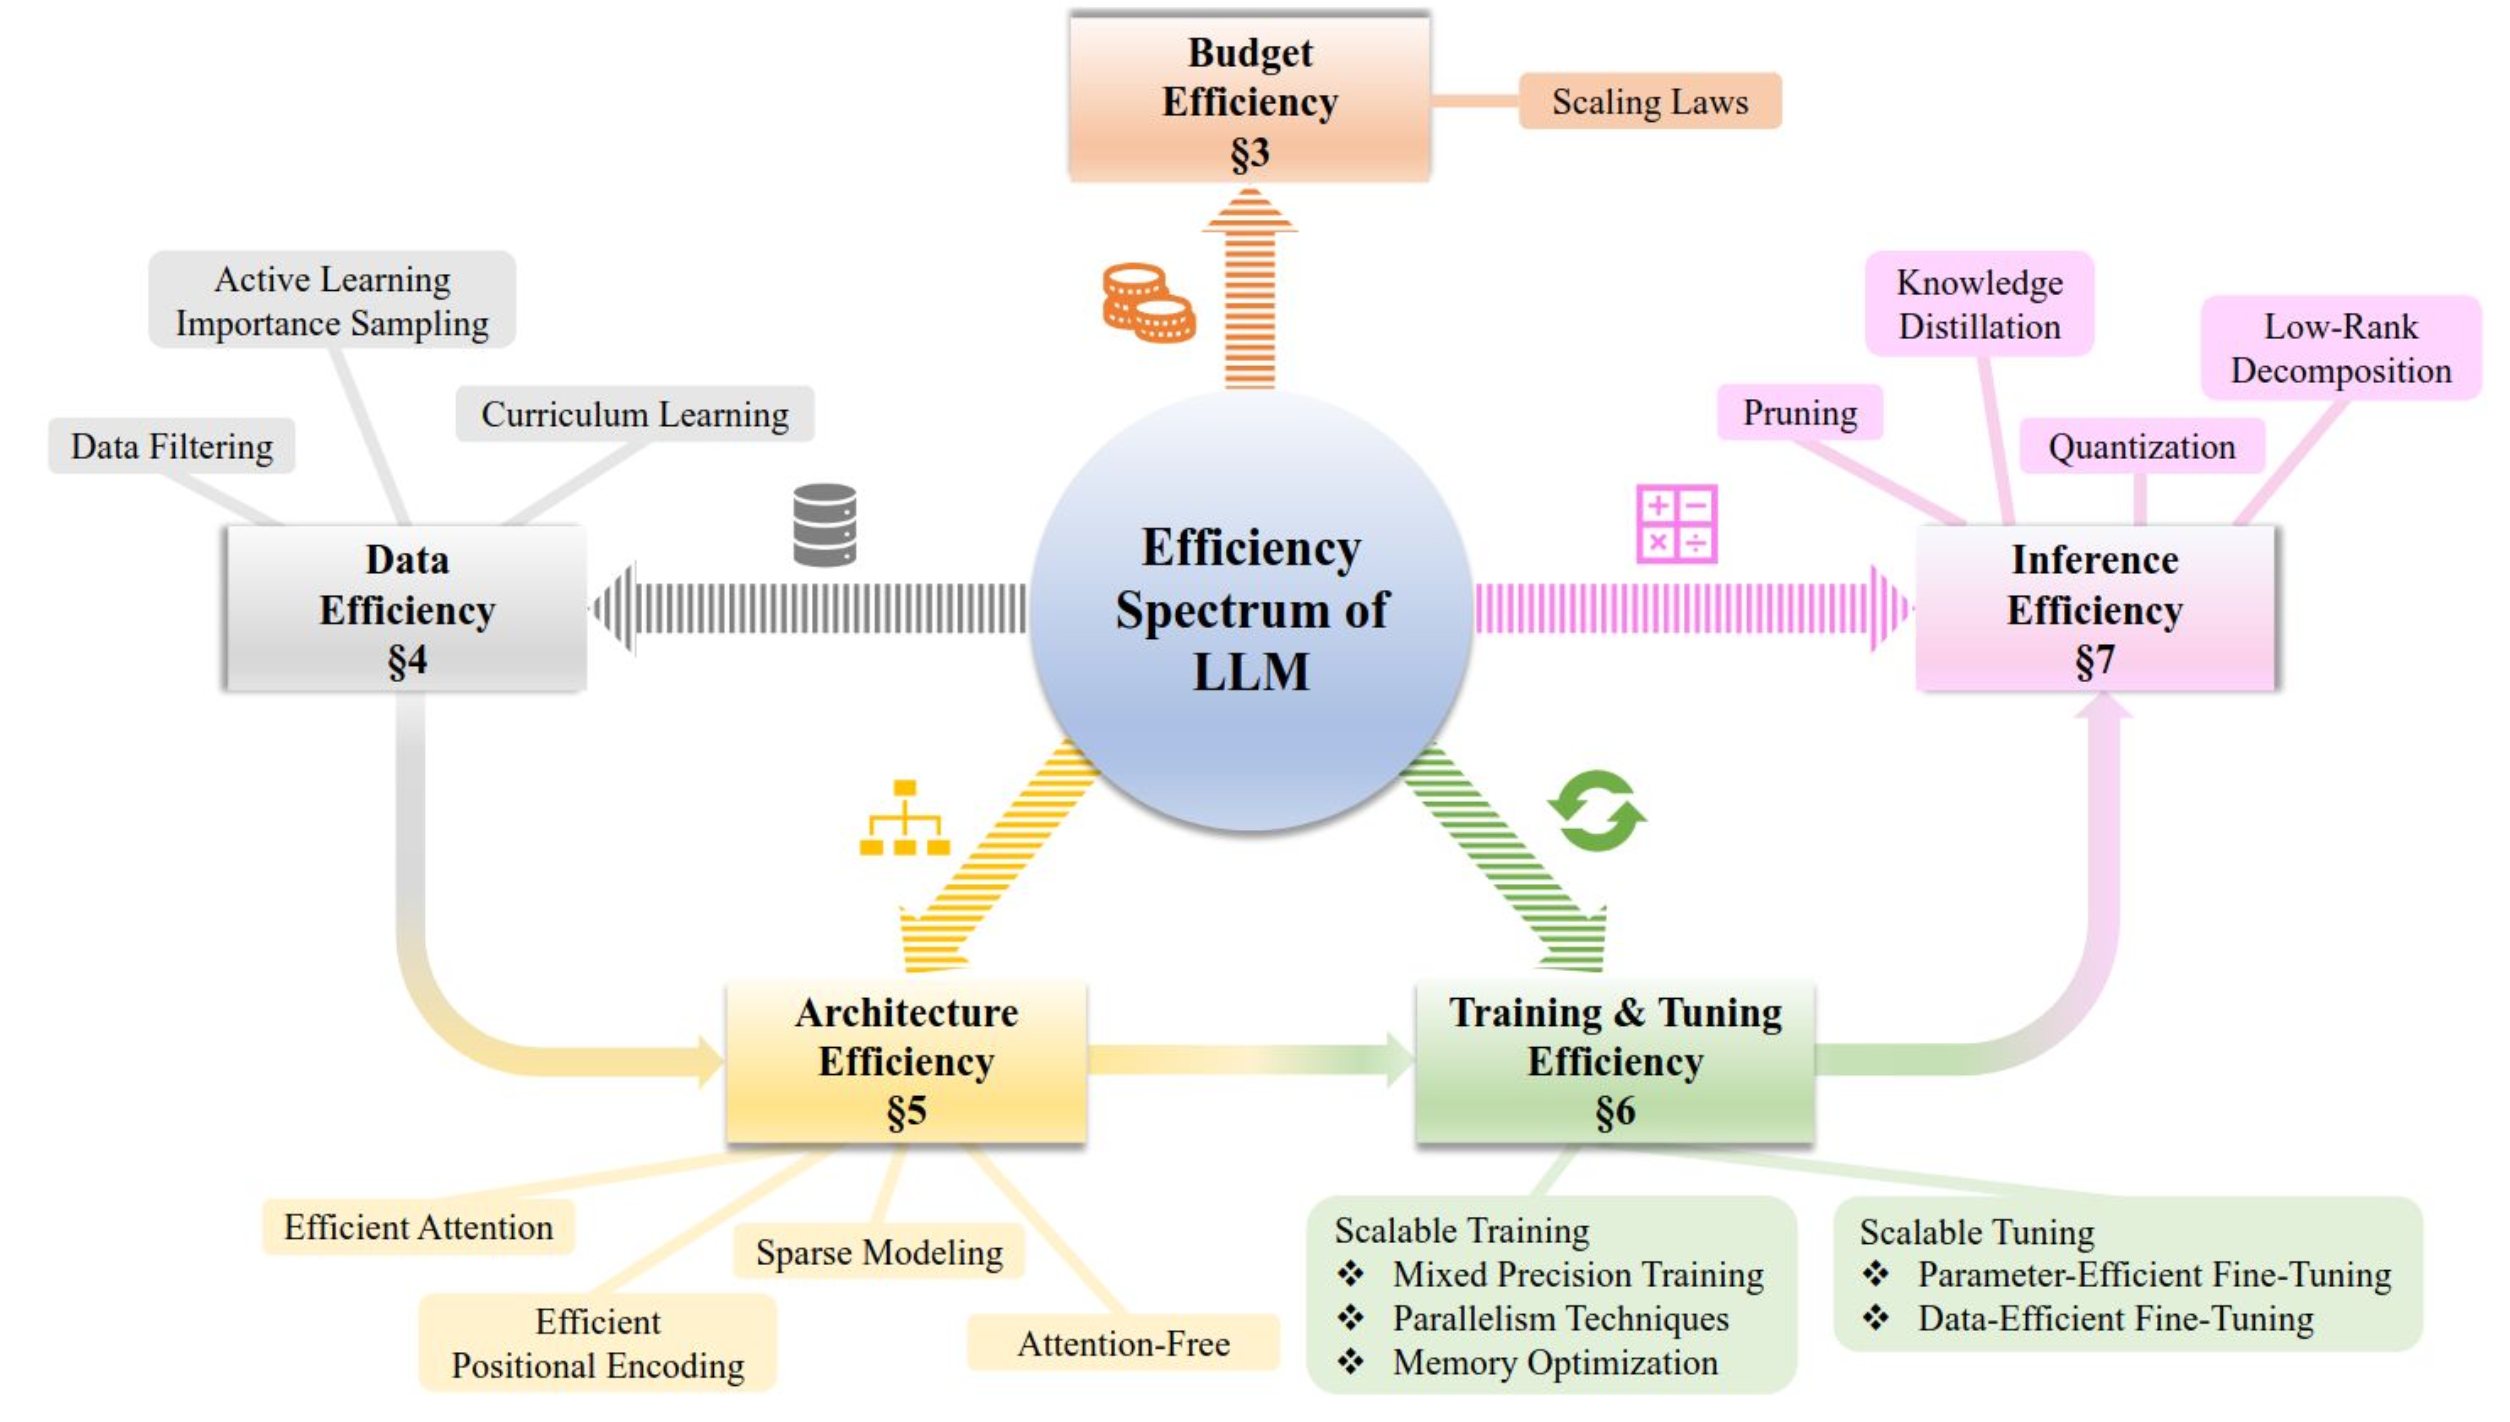
\includegraphics[width=\linewidth]{cs4248-recent-efficiency.png} 
  \begin{itemize}
    \item More params \textrightarrow better model, but: \textit{increased} memory requirements, training \& inferencing time, energy consumption, need for more data, \dots
    \item Scaling laws:
    \item \begin{itemize}
      \item Bigger not always better.
      \item Model performance follows a power law improvement with increasing \#params. (insufficient data)
      \item Performance scales predictably with compute until hits hardware/data limits.
    \end{itemize}
  \end{itemize}
  
  \subsection{Quantization}
  \begin{itemize}
    \item Core idea: Reduce the numerical precision of the model weights and activations (Mostly \textbf{PTQ}: post-training quantization).
    \item Advantages: reduced memory requirements, faster calculations.
    \item Disadvantages: risk of accuracy degradation, trickier to implement (not suitable for all layers).
    \item \textbf{Goals}: 
    \item \begin{itemize}
      \item Map high-precision values to low-precision values of a smaller range.
      \item Preserve overall distribution of the values.
    \end{itemize}
  \end{itemize}
  \subsubsection{Asymmetric quantization}
  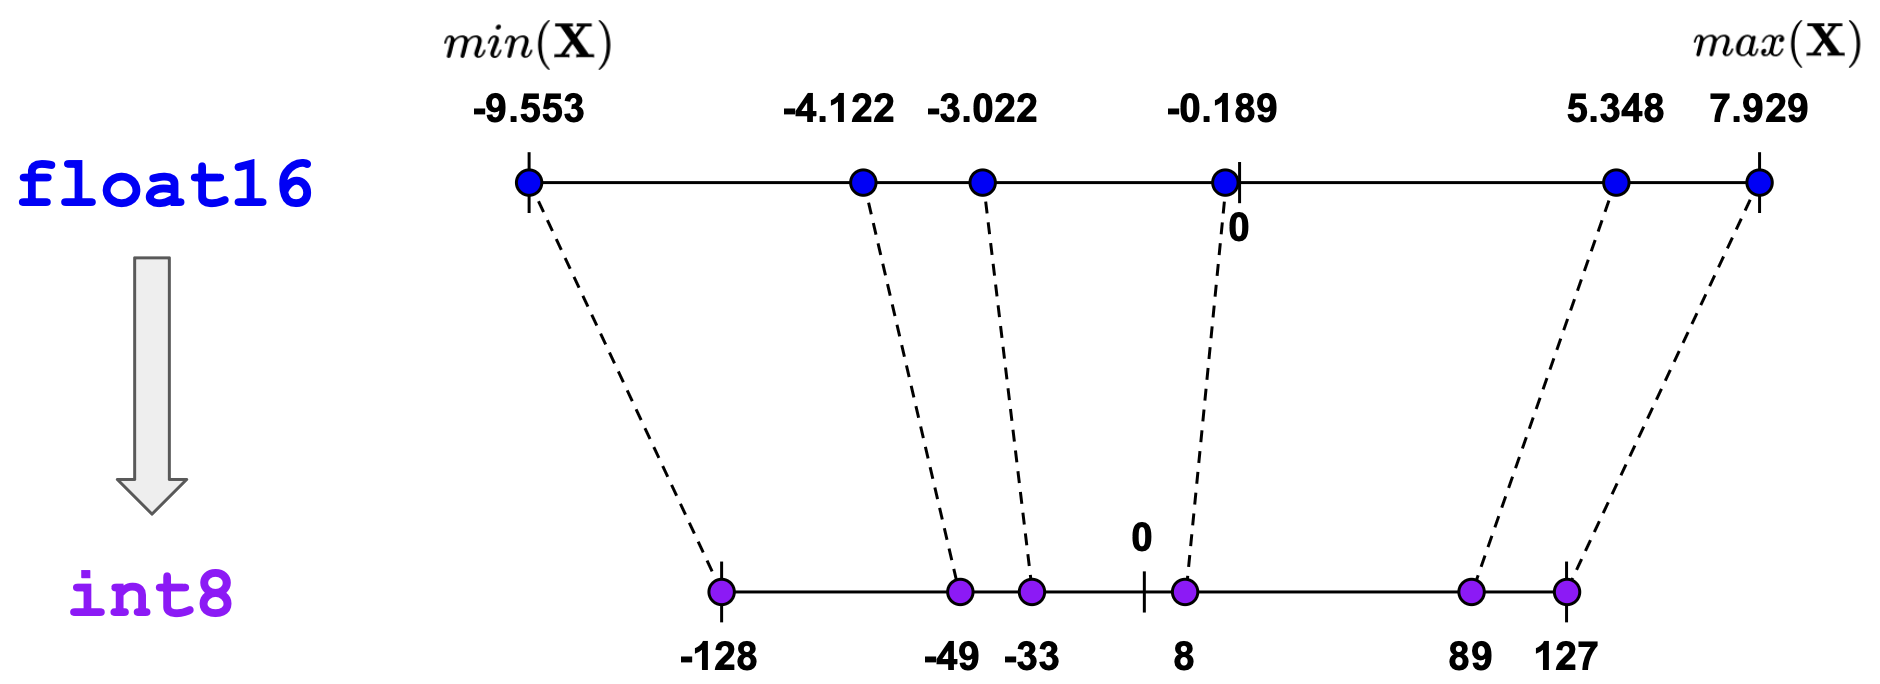
\includegraphics[width=\linewidth]{cs4248-recent-quantize.png}
  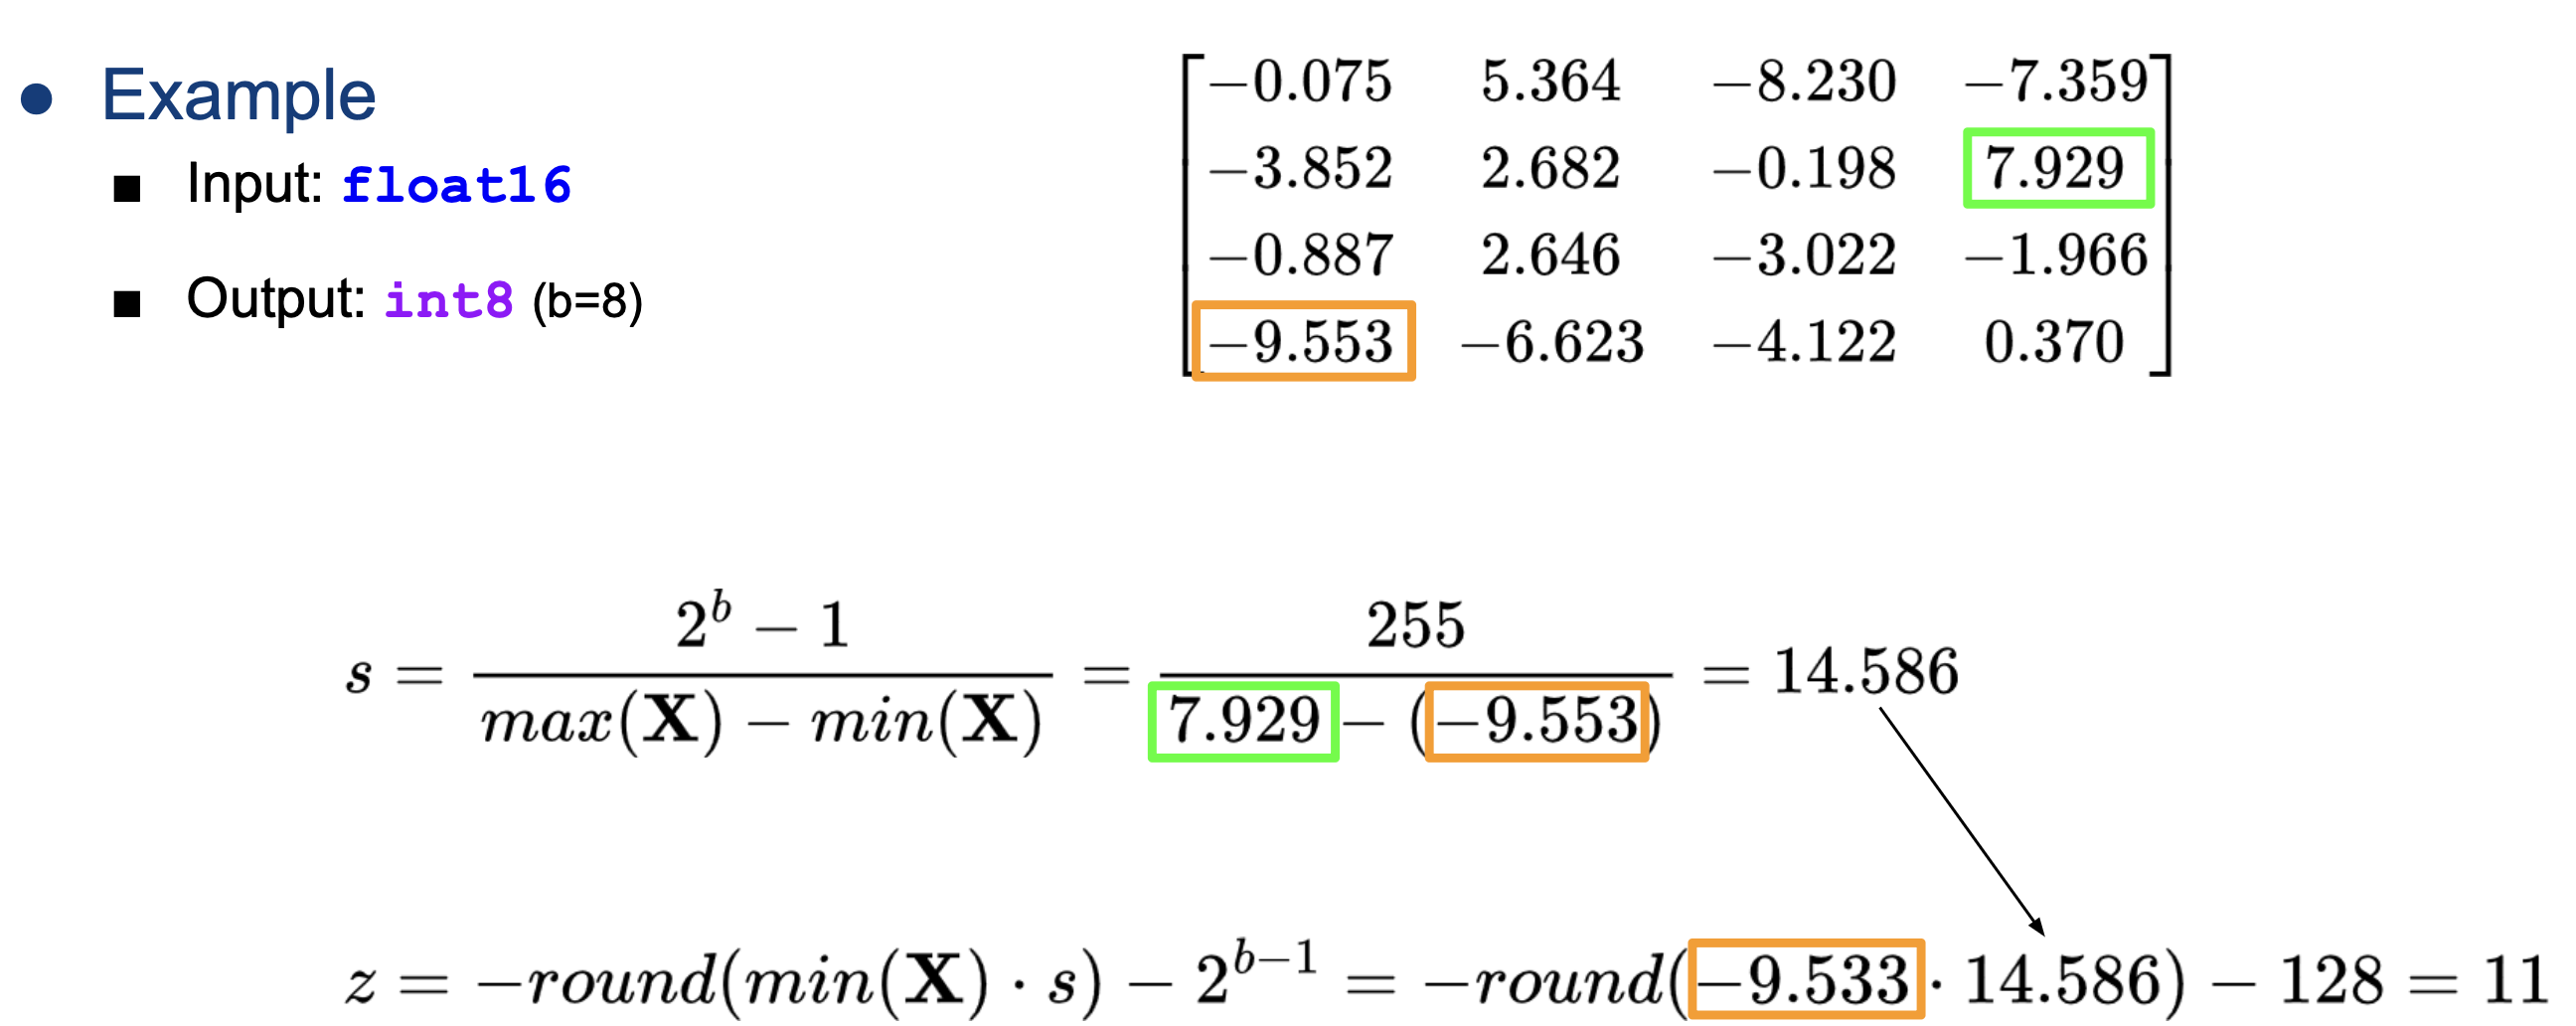
\includegraphics[width=\linewidth]{cs4248-recent-asy-quant.png}
  \begin{itemize}
    \item Quantization: $X_{quant} = X \cdot s + z$
    \item Dequantization: $X_{dequant} = (X_{quant} - z)/s$
    \item \textbf{Handling outliers}:
    \item \begin{itemize}
      \item Clipping: clip the values to a certain range.
      \item Calibrate the clipping range:
      \item \begin{itemize}
        \item static calibration: find best ranges before inferences using a calibration dataset
        \item dynamic calibration: after each layer, collect statistics of activations to find best ranges
      \end{itemize}
    \end{itemize}
  \end{itemize}
  \subsubsection{Quantization-aware training (QAT)}
  \begin{itemize}
    \item Idea: Simulate quantization during training.
    \item \textbf{FakeQuant nodes} between the layers: quantize and immediately dequantize the values.
    \item Model is still trained with high-precision values under the hood.
  \end{itemize}
  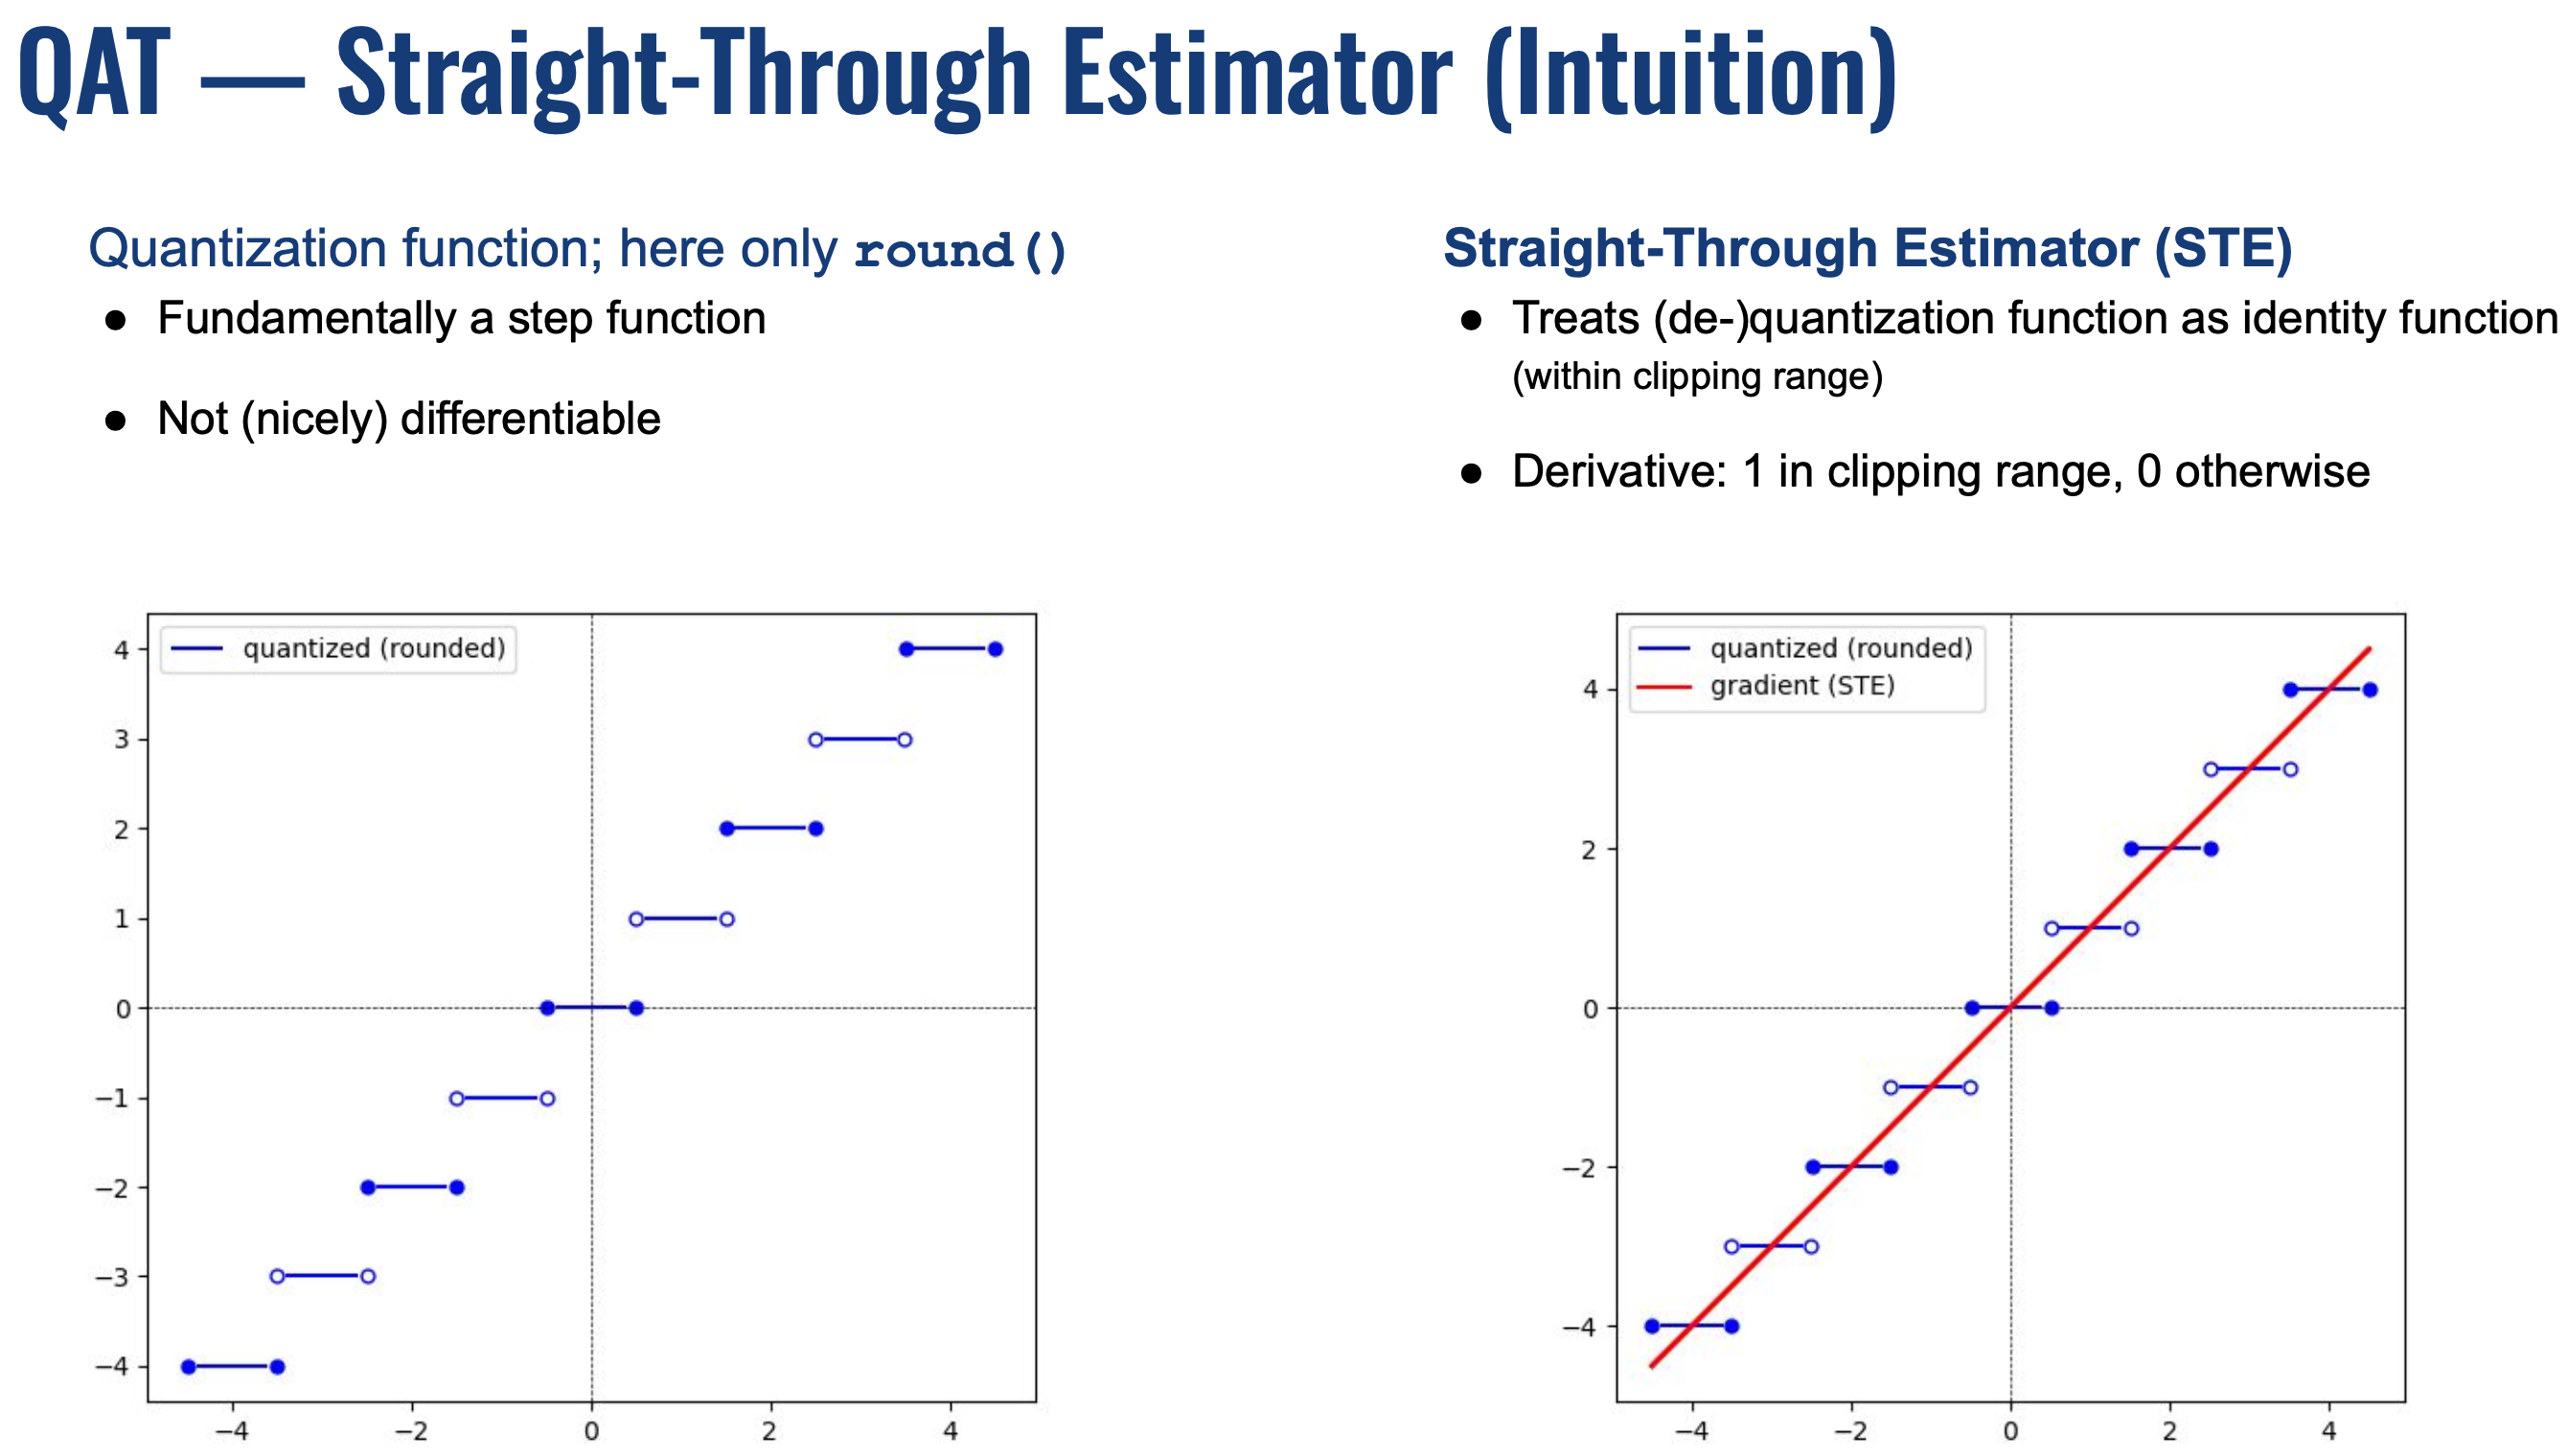
\includegraphics[width=\linewidth]{cs4248-recent-ste.png}
  \subsubsection{KV caching}
  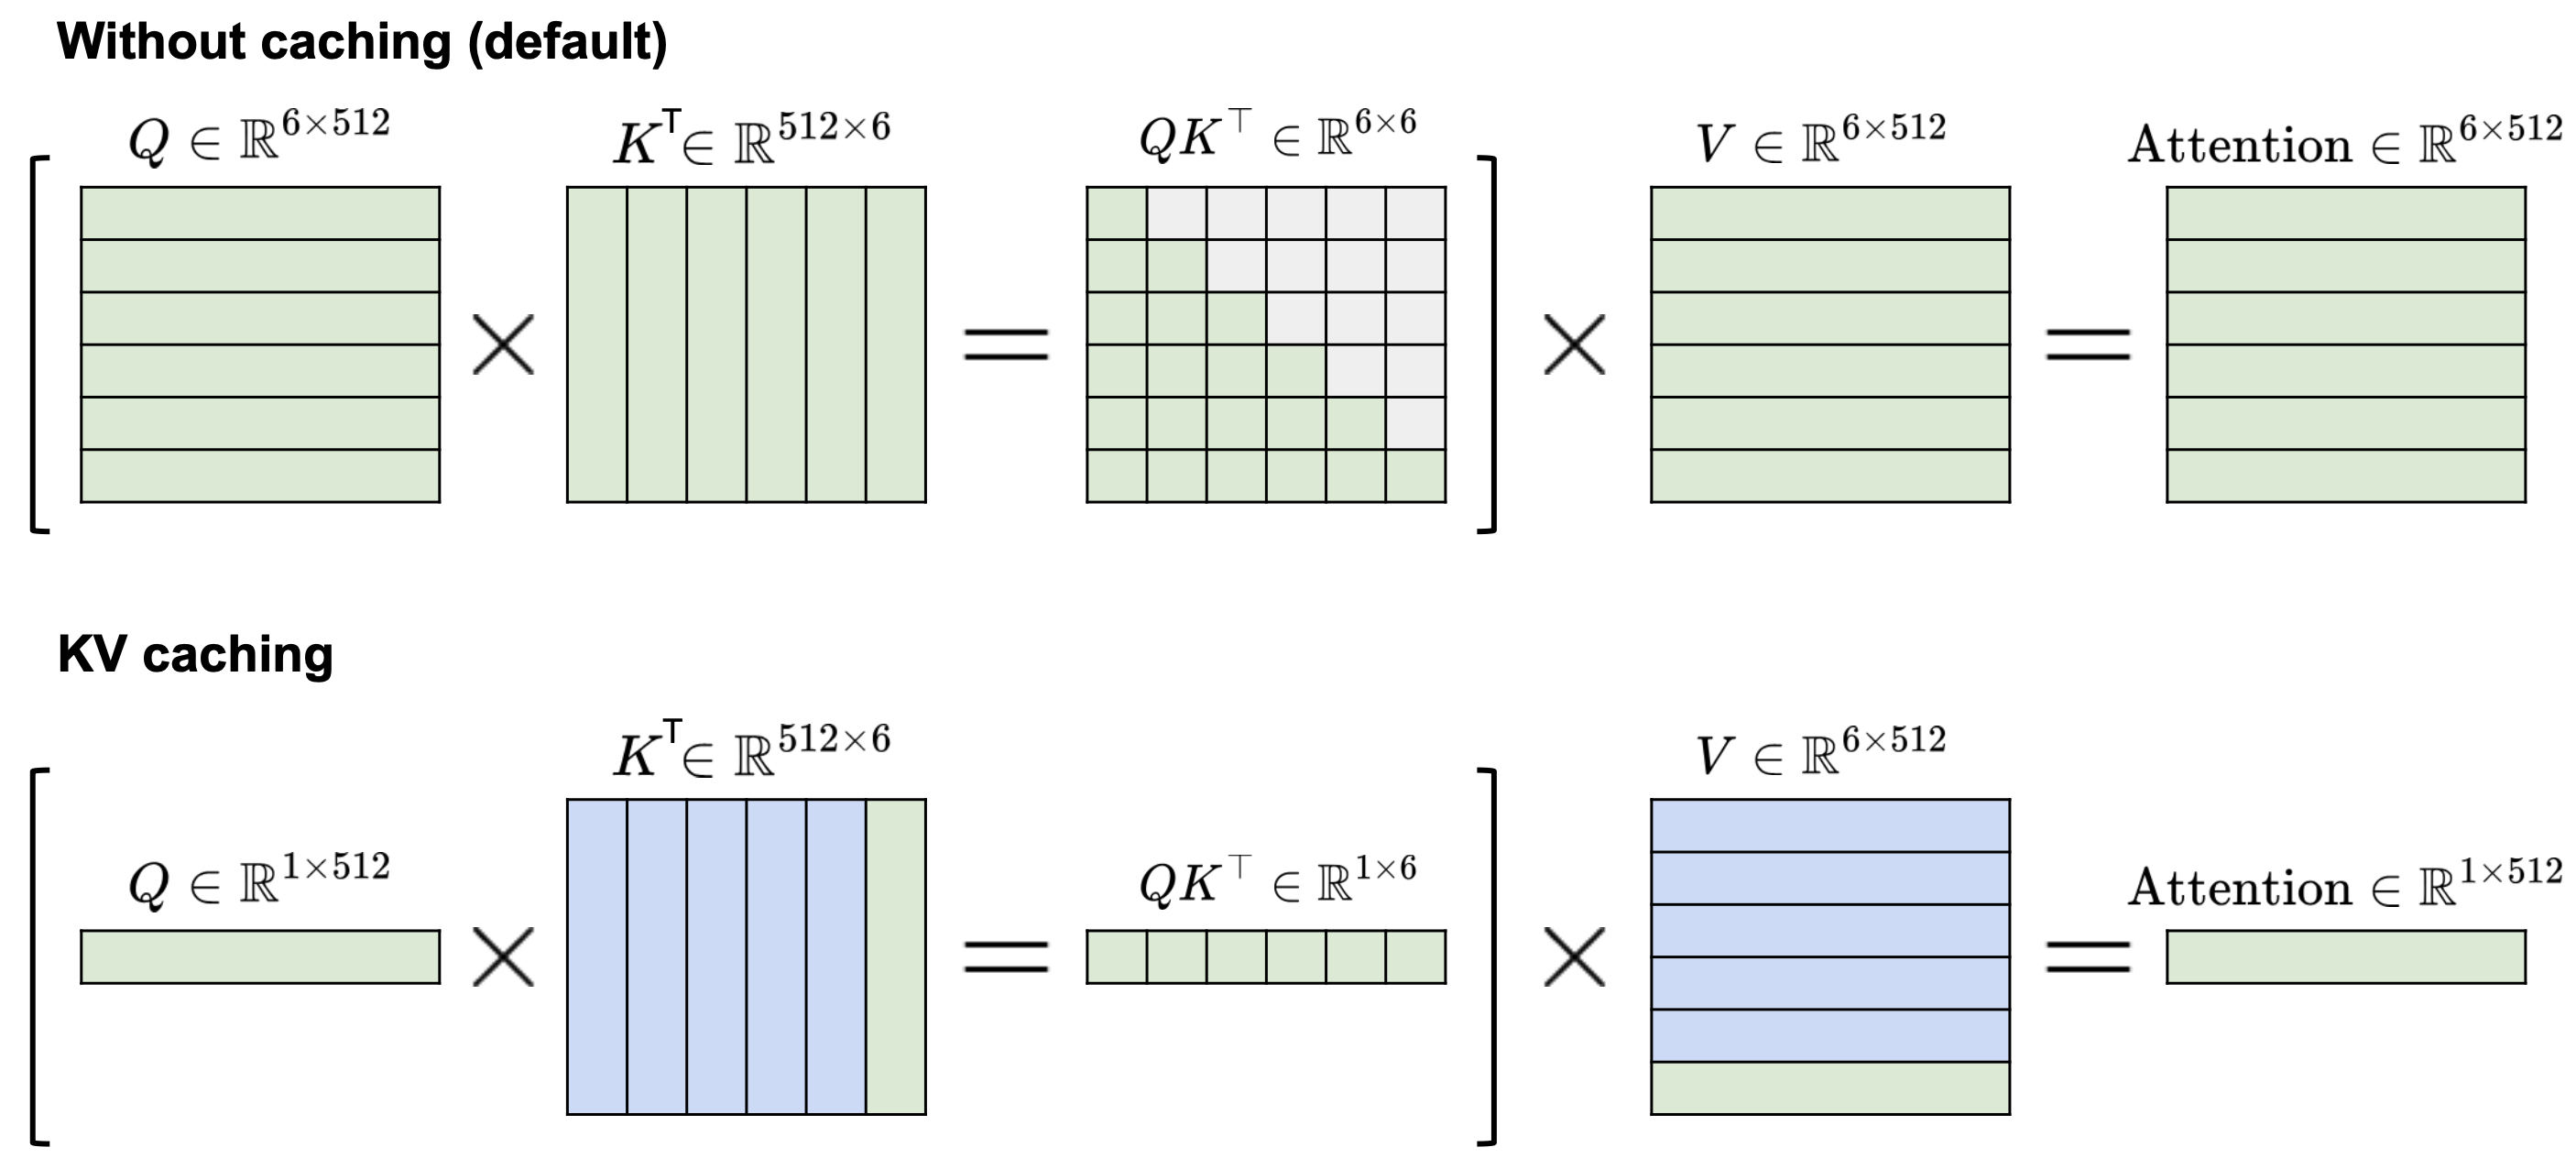
\includegraphics[width=\linewidth]{cs4248-recent-kvcaching.png}
  \begin{itemize}
    \item Cache size formula: $2\cdot n\cdot b\cdot t\cdot \underbrace{(d\cdot h)}_{d_{model}} \cdot p$
    \item Example (fp16): $2\cdot 32\cdot 32\cdot 500\cdot (128\cdot 32) \cdot 2 \approx 7.81\text{GB}$
    \item \textbf{Memory optimization}: 
    \item \begin{itemize}
      \item Basic strategies: Reduce model size, reduce precision (both potentially reduce accuracy); reduce batch size (reduces efficiency).
      \item Advanced strategies: attention variants
      \item \textbf{Grouped-query/multi-query attention}: 
      \item 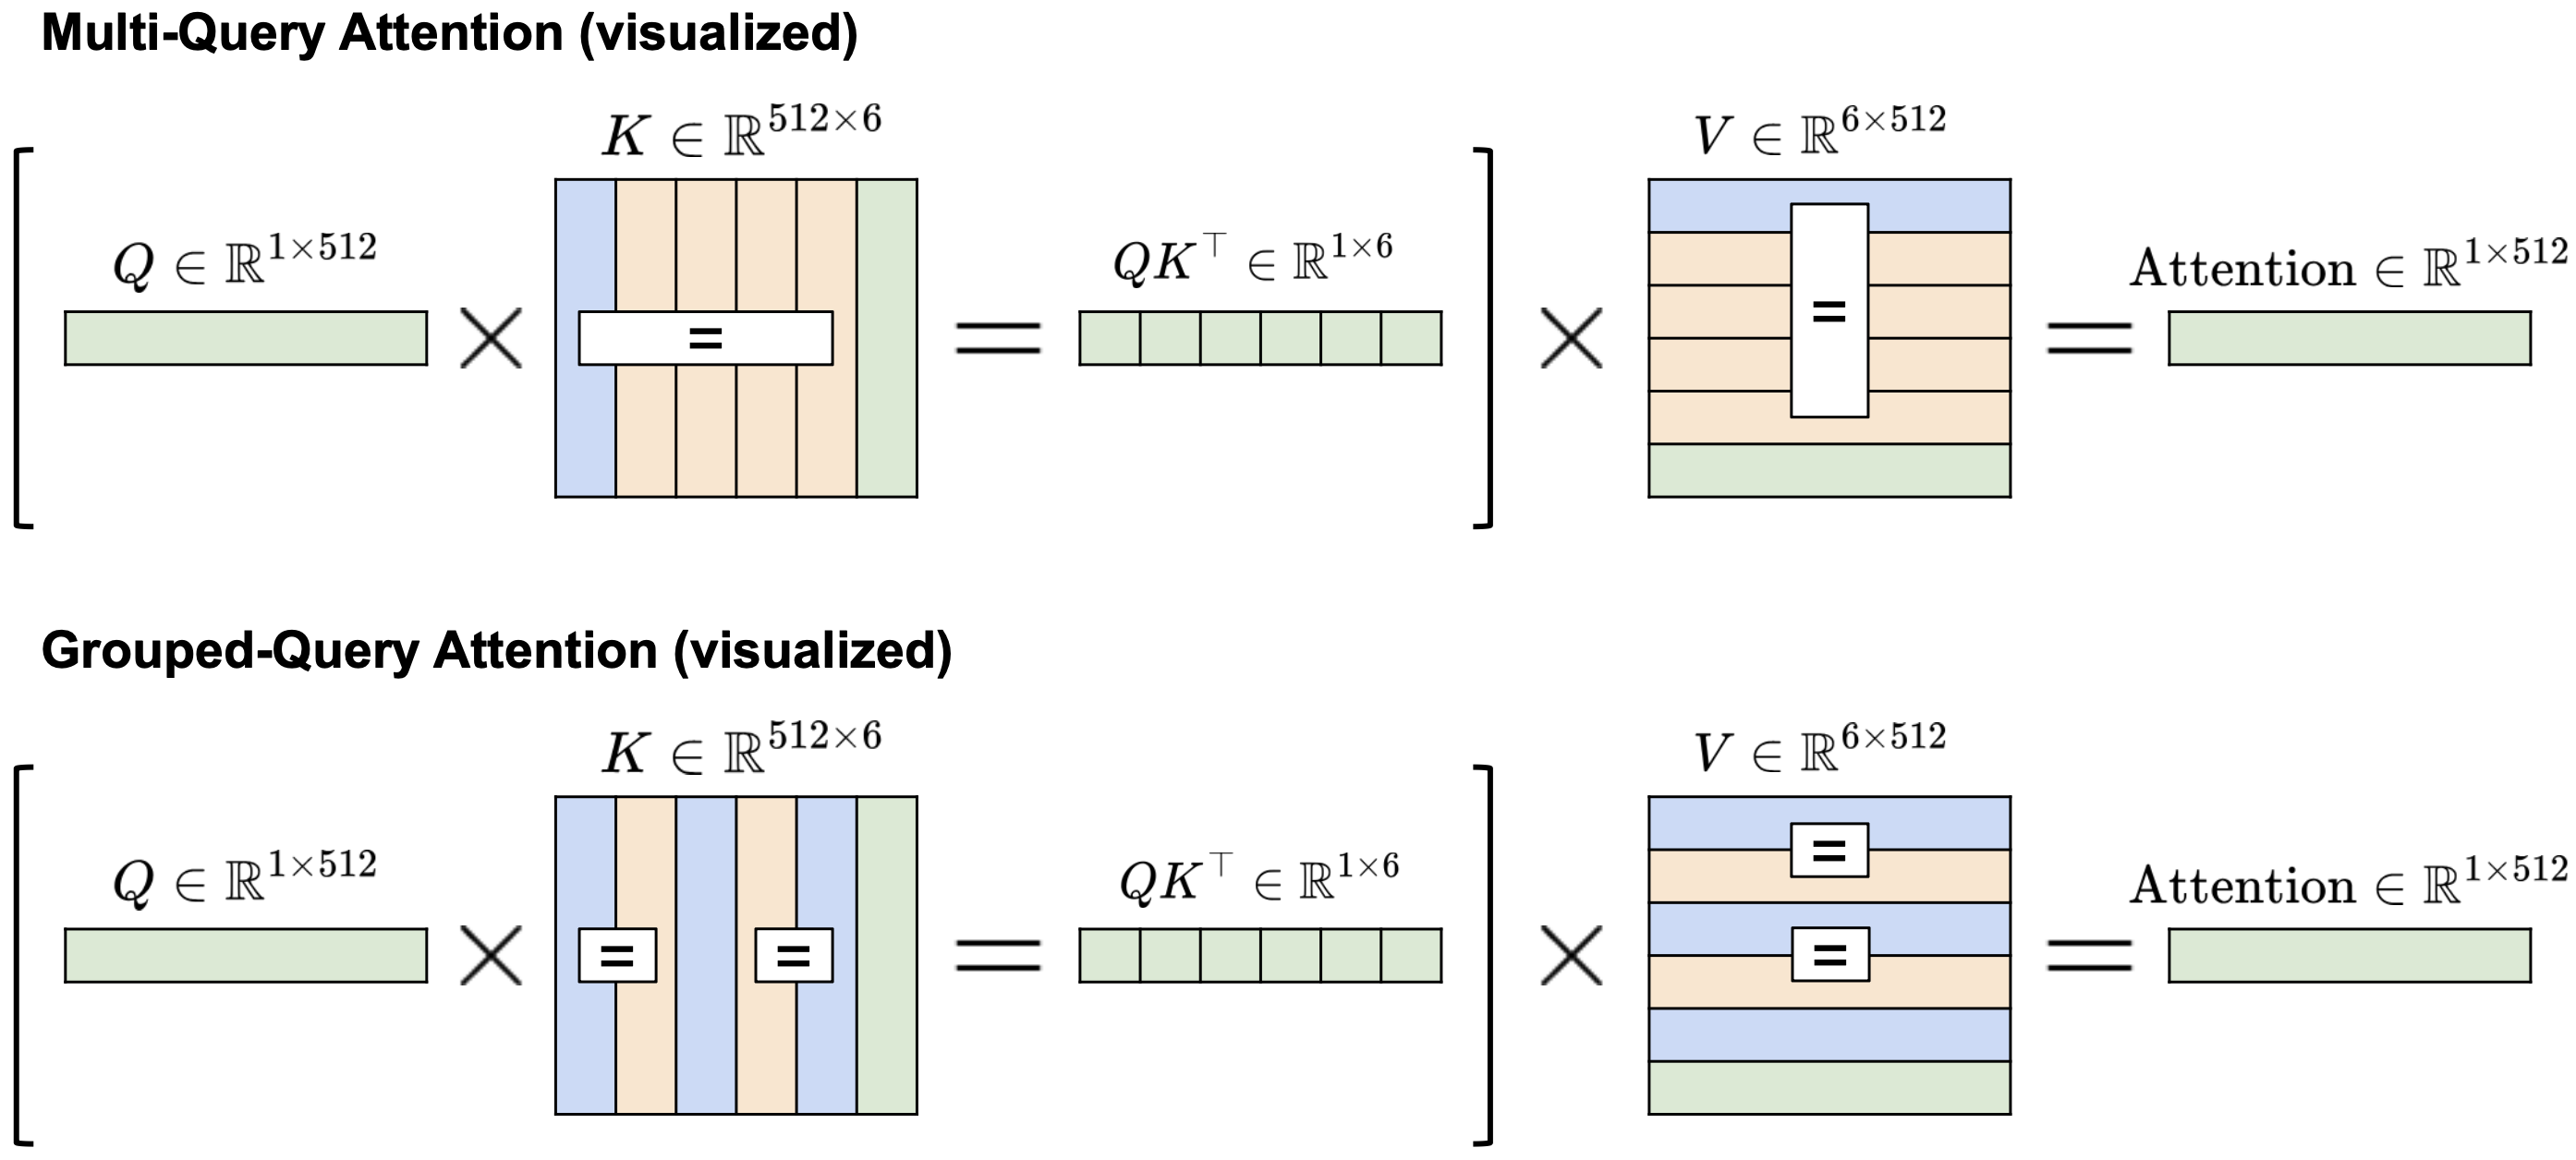
\includegraphics[width=\linewidth]{cs4248-recent-multiquery.png}
      \item \textbf{Multi-head latent attention}:
      \item 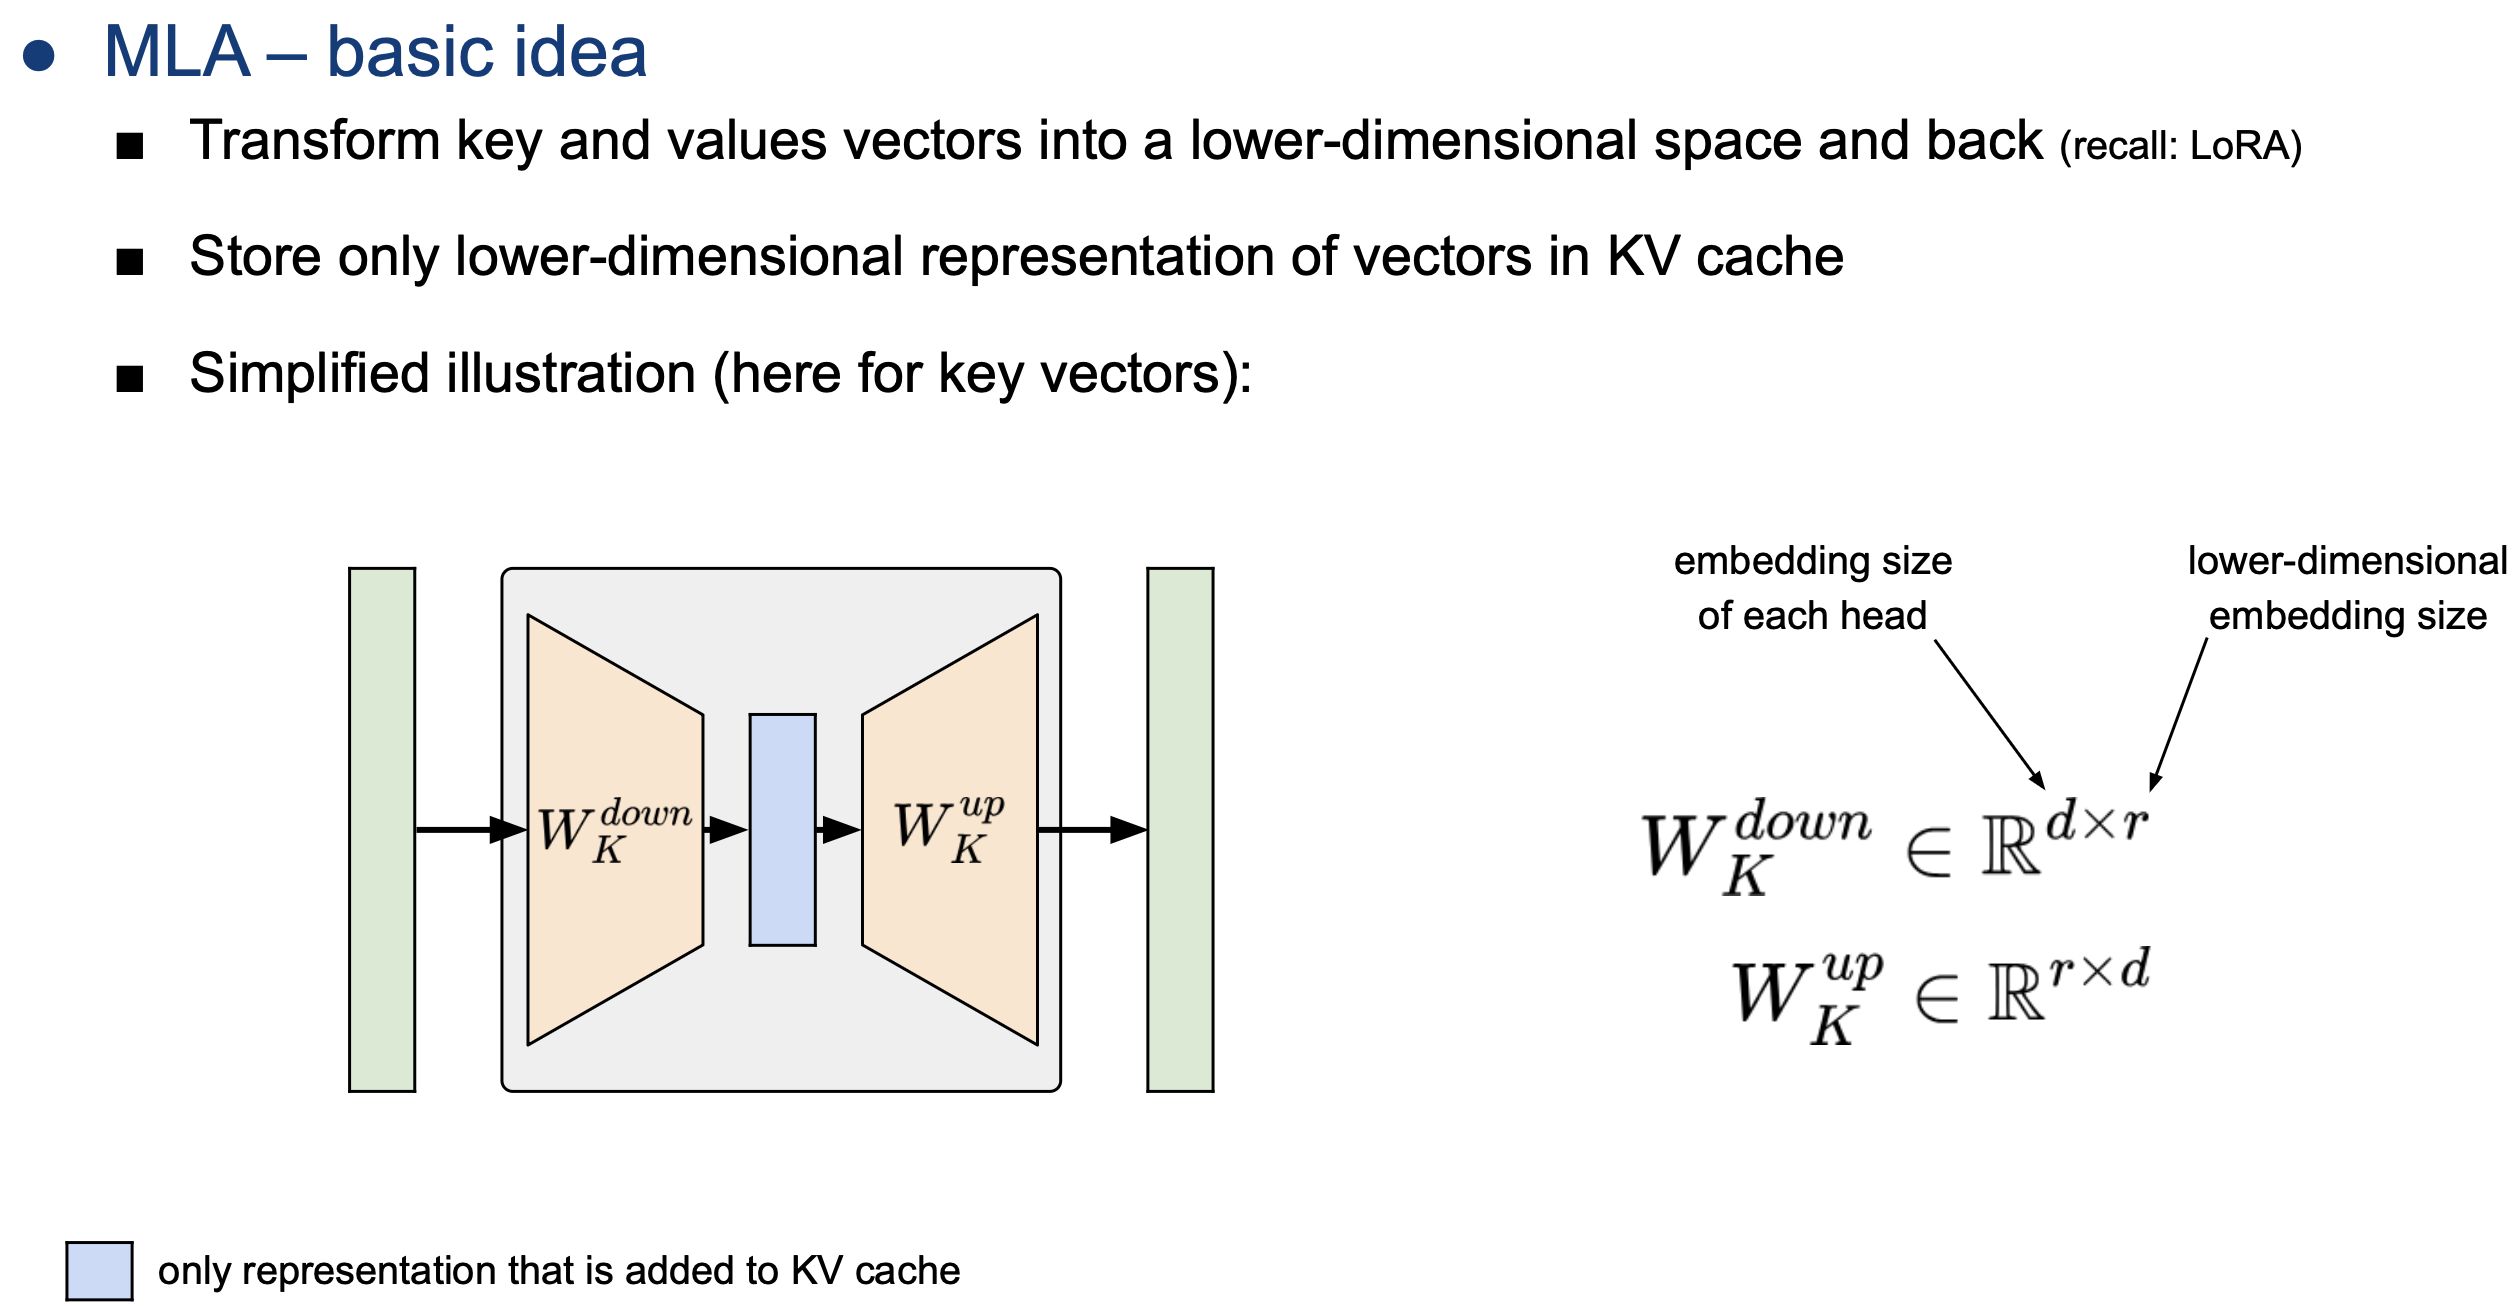
\includegraphics[width=\linewidth]{cs4248-recent-mla.png}
    \end{itemize}
    \subsubsection{Mixture of experts}
    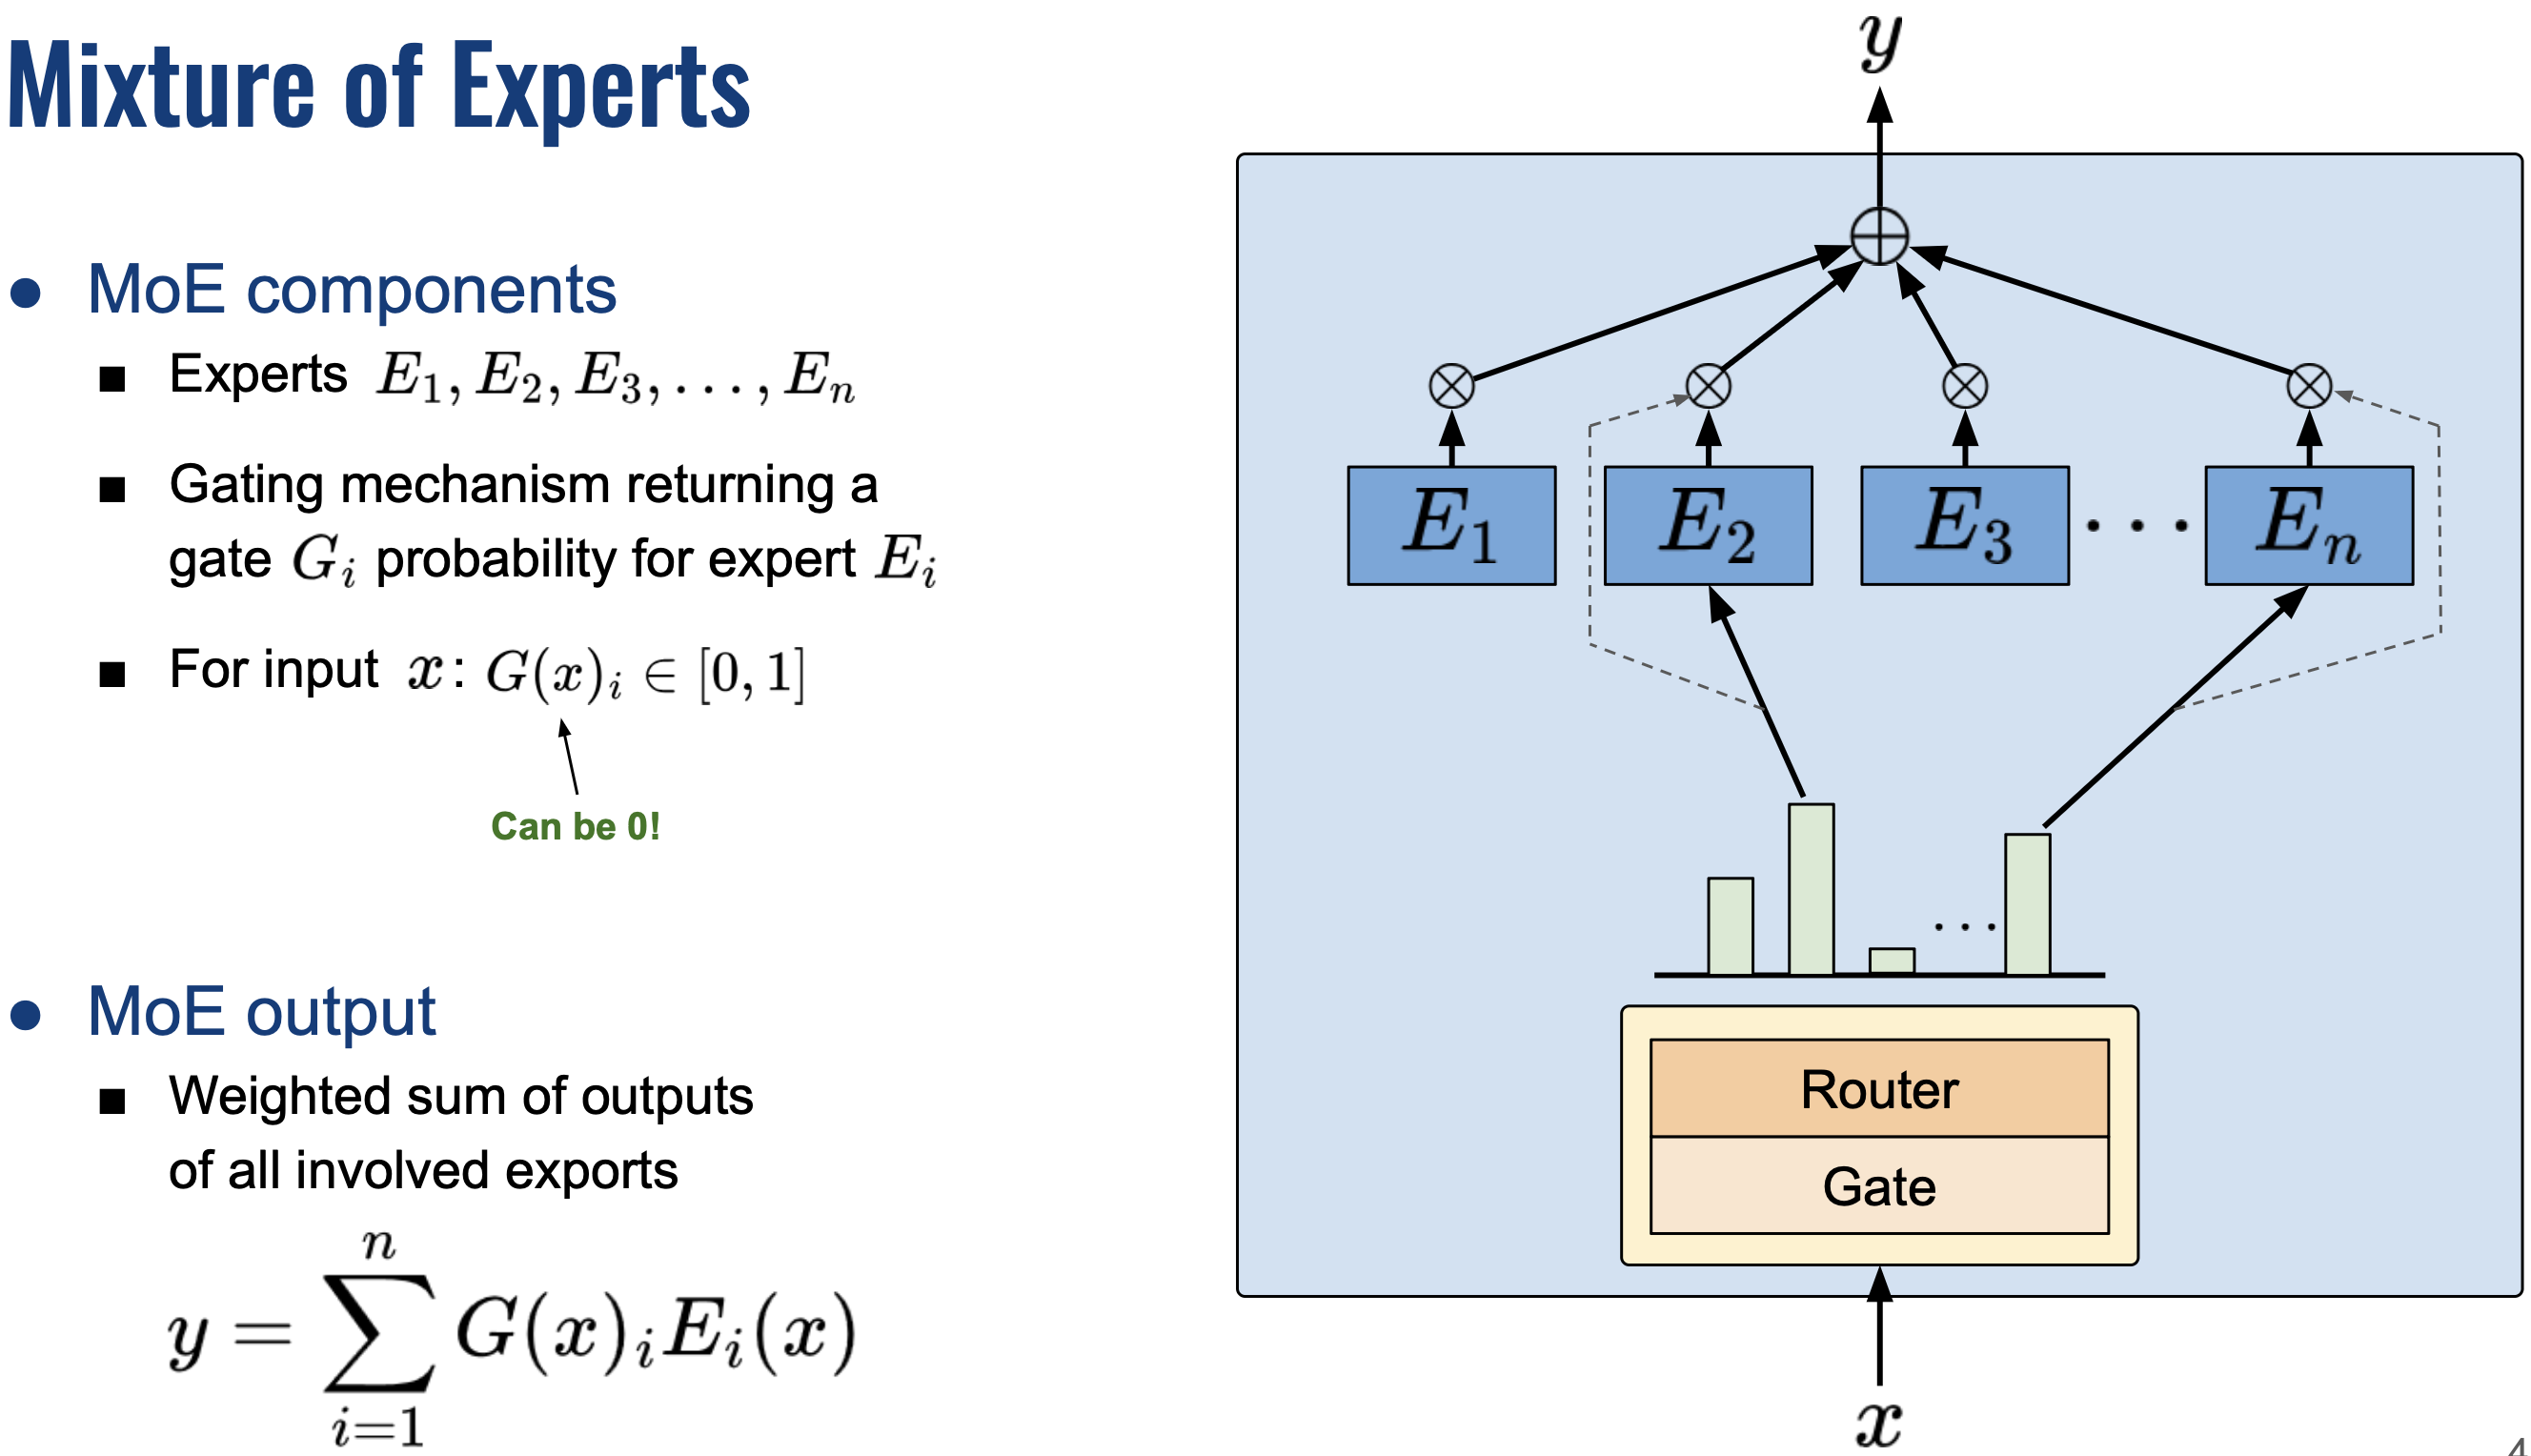
\includegraphics[width=\linewidth]{cs4248-recent-moe.png}
    \begin{itemize}
      \item Expert: Architecture can be anything (even a mixture of different architectures).
      \item Gate: e.g. a FFNN that returns logits/softmax probabilities.
      \item Router: subnetwork that decides which experts to pass the input to based on the gate's output and other information.
      \item \textbf{Dense MoE}: Use all experts' outputs and mix based on the gate's probabilities.
      \item \textbf{Sparse MoE}: Inputs are only passed to the experts with the highest gate probabilities (e.g. top-2). Outputs are a weighted sum (rescaled) of the chosen experts' outputs.
      \item 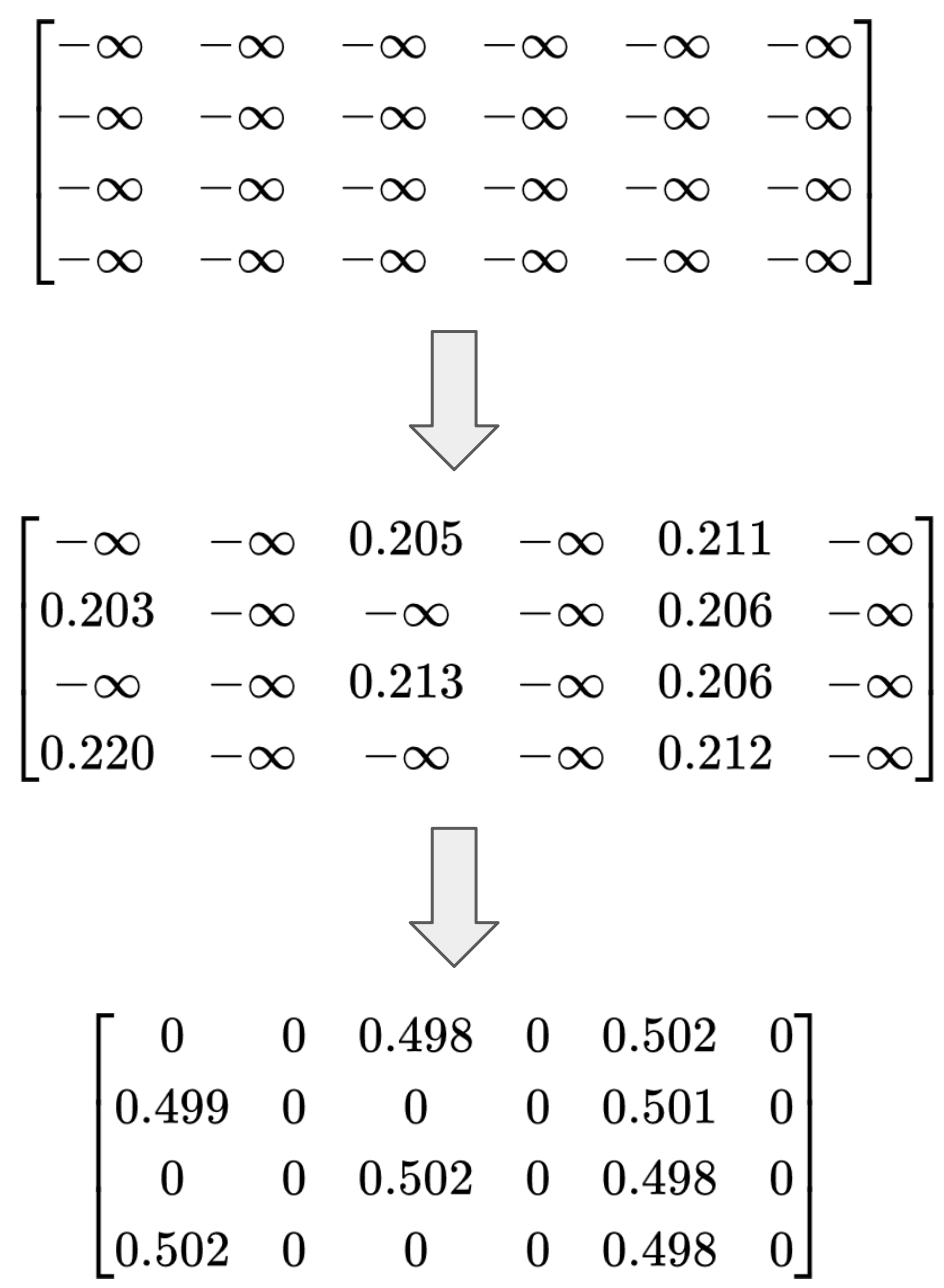
\includegraphics[width=0.4\linewidth]{cs4248-recent-topk.png}
      \columnbreak
      \item Limitations:
      \item \begin{itemize}
        \item Gating mechanism often selects only the most prominent experts. Model will be underutilized, may degrade overall performance of model. Reduces diversity in learning and limits the specialization of different experts.
      \end{itemize}
      \item \textbf{Stochastic routing}:
      \item \begin{itemize}
        \item Gives all experts a chance to be selected early in training: (passive) load balancing
        \item Adding of noise can be a tunable operation by introducing additional learnable parameters
        \item $G(x) = Softmax(TopK(H(x), k))$ $H(x) = (\mathbf{W}_{gate}\mathbf{x}) + StandardNormal() \cdot SoftPlus(\mathbf{W}_{noise}\mathbf{x})$
        \item \textbf{SoftPlus}:\\
        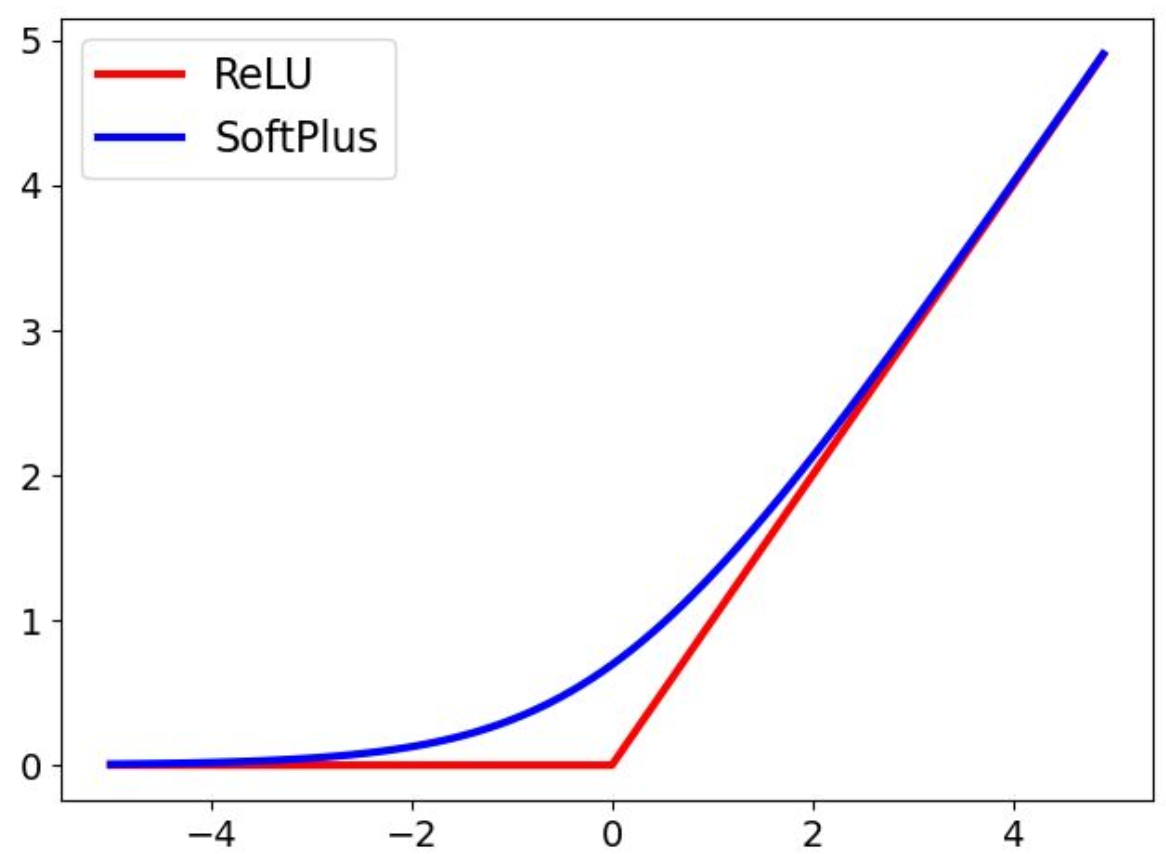
\includegraphics[width=0.6\linewidth]{cs4248-recent-softplus.png}
        \item Smooth and differentiable approximation of ReLU, makes optimization more stable and always positive.
      \end{itemize}
      \item \textbf{Load balancing}:
      \item 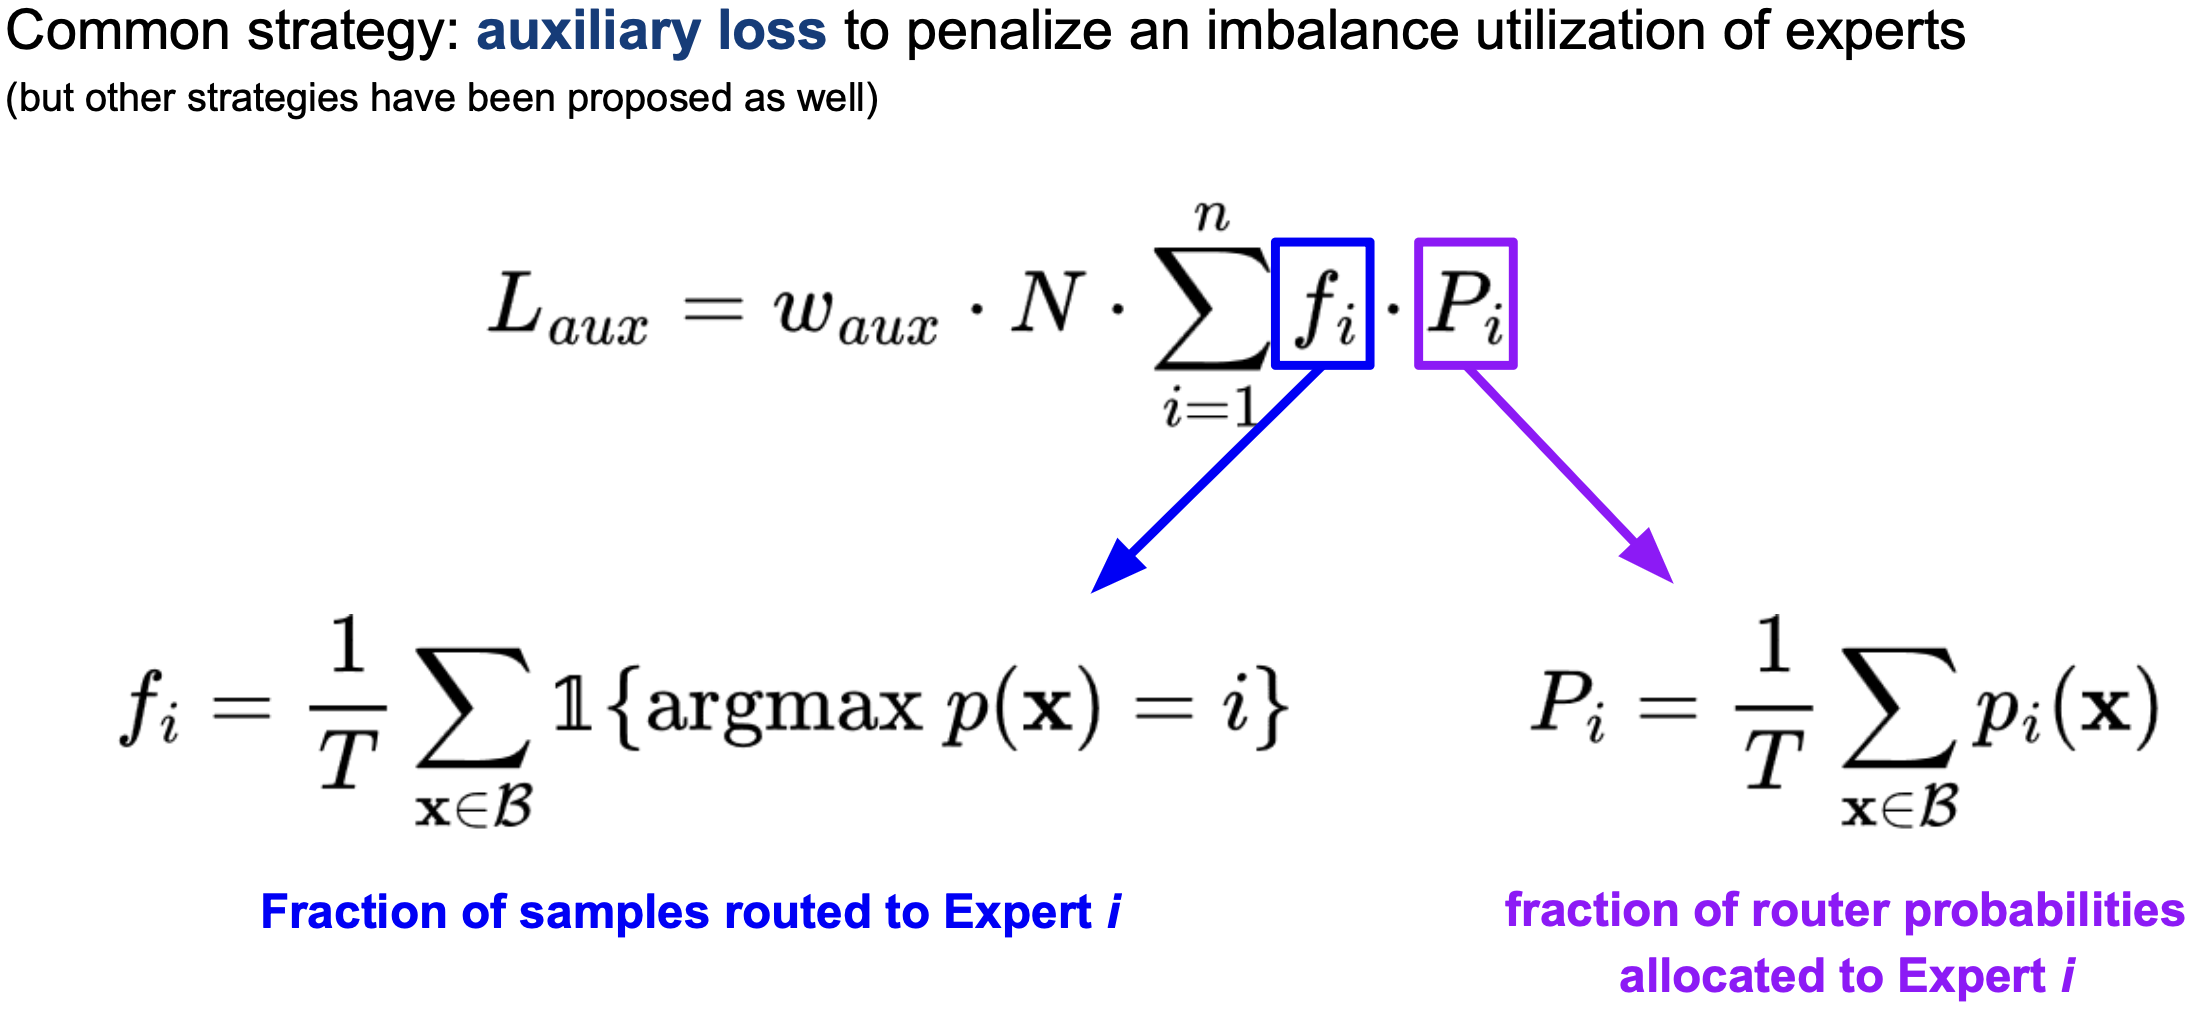
\includegraphics[width=\linewidth]{cs4248-recent-auxloss.png}
    \end{itemize}
    \pagebreak
    \subsubsection{Distillation}
    \begin{itemize}
      \item Motivation: Large LLMs are expensive to train and run.
      \item \textbf{Response distillation}: Teacher LLM labels the training data and the student LLM learns from the teacher's labels. Limitations: good teacher \& dataset needed, expensive, no nuanced knowledge, less creative.
      \item \textbf{Logit distillation}: 
      \item \begin{enumerate}
        \item Give same data to teacher and student.
        \item Minimize the KL divergence (\textbf{distillation loss}) between the teacher and student logits.
      \end{enumerate}
      \begin{itemize}
        \item Advantages: no need for labelled data, nuances captured through logits.
        \item Disadvantages: teacher's biases inherited by student, missing ground truth for evaluation.
      \end{itemize}
      \item Variation:\\ 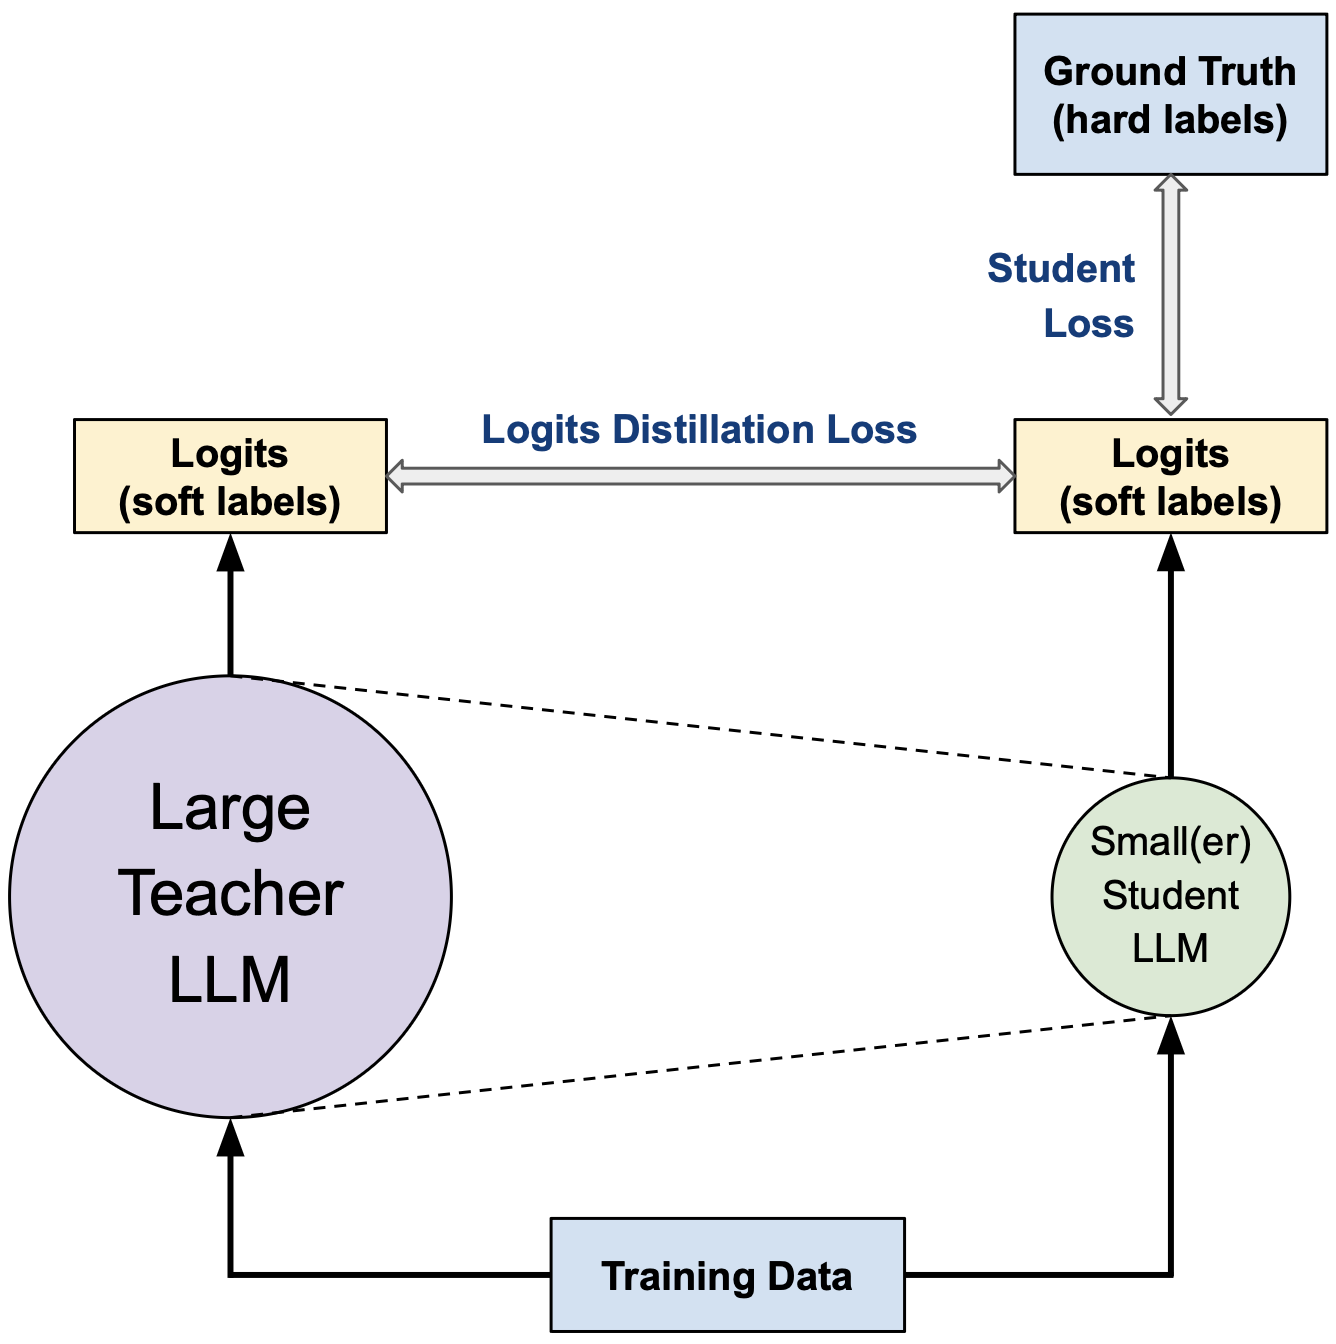
\includegraphics[width=0.6\linewidth]{cs4248-recent-logitdistill.png}
      \item \begin{itemize}
        \item Also calculate the "normal" loss based on the labelled dataset.
        \item Advantages: richer training signal, more stable training, straightforward evaluation.
        \item Limitations: added complexity, conflicting signals, non-obvious combination of losses.
      \end{itemize}
      \item \textbf{Feature distillation}: \\ 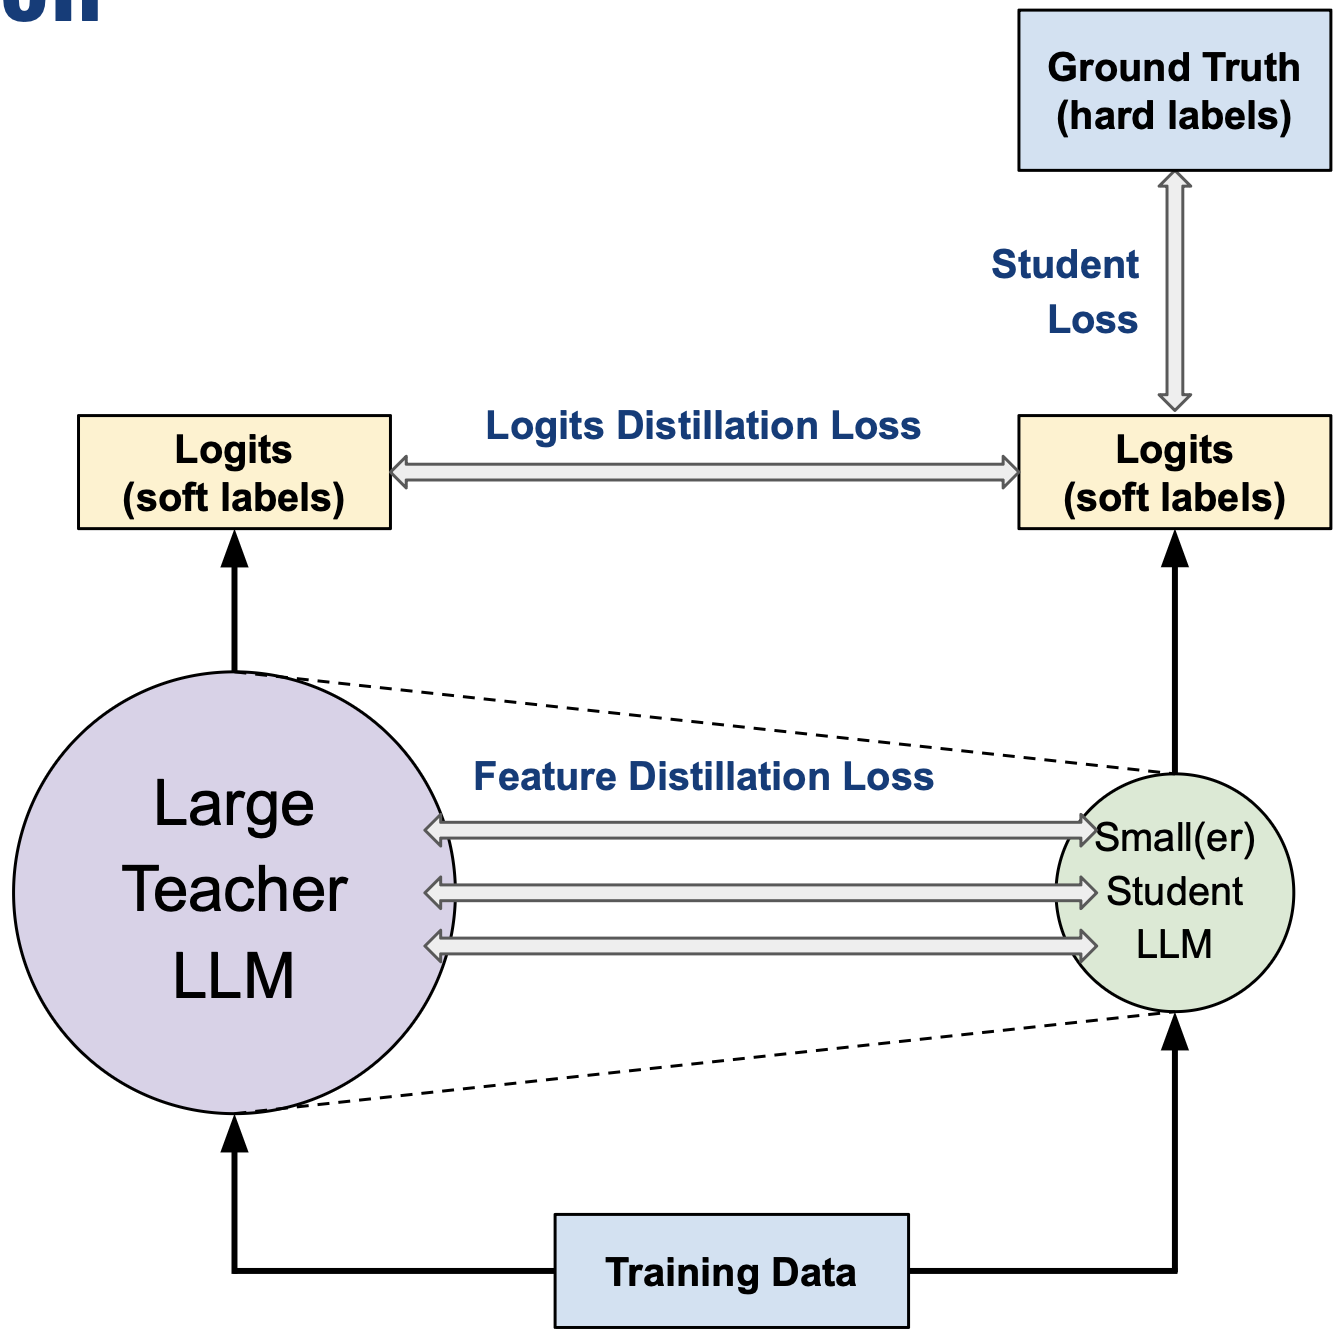
\includegraphics[width=0.6\linewidth]{cs4248-recent-featuredistill.png}
      \item \begin{itemize}
        \item Student learns to mimic the teacher's intermediate representations.
        \item Limitations: non-trivial layer alignment for different architectures.
      \end{itemize}
      \item \textbf{Question}: Why logits but not softmax probabilities? It is because the raw logits better preserve the relative confidence of the teacher model.
    \end{itemize}
  
  \end{itemize}
\end{multicols*}
\end{document}